
% ------------------ DOCUMENT SETUP ------------------ 
% The document class defines the document type (report) and sets the font size (10pt)
\documentclass{report}

% Optional math commands from https://github.com/goodfeli/dlbook_notation.
%%%%% NEW MATH DEFINITIONS %%%%%

\usepackage{amsmath,amsfonts,bm}

% Mark sections of captions for referring to divisions of figures
\newcommand{\figleft}{{\em (Left)}}
\newcommand{\figcenter}{{\em (Center)}}
\newcommand{\figright}{{\em (Right)}}
\newcommand{\figtop}{{\em (Top)}}
\newcommand{\figbottom}{{\em (Bottom)}}
\newcommand{\captiona}{{\em (a)}}
\newcommand{\captionb}{{\em (b)}}
\newcommand{\captionc}{{\em (c)}}
\newcommand{\captiond}{{\em (d)}}

% Highlight a newly defined term
\newcommand{\newterm}[1]{{\bf #1}}


% Figure reference, lower-case.
\def\figref#1{figure~\ref{#1}}
% Figure reference, capital. For start of sentence
\def\Figref#1{Figure~\ref{#1}}
\def\twofigref#1#2{figures \ref{#1} and \ref{#2}}
\def\quadfigref#1#2#3#4{figures \ref{#1}, \ref{#2}, \ref{#3} and \ref{#4}}
% Section reference, lower-case.
\def\secref#1{section~\ref{#1}}
% Section reference, capital.
\def\Secref#1{Section~\ref{#1}}
% Reference to two sections.
\def\twosecrefs#1#2{sections \ref{#1} and \ref{#2}}
% Reference to three sections.
\def\secrefs#1#2#3{sections \ref{#1}, \ref{#2} and \ref{#3}}
% Reference to an equation, lower-case.
\def\eqref#1{equation~\ref{#1}}
% Reference to an equation, upper case
\def\Eqref#1{Equation~\ref{#1}}
% A raw reference to an equation---avoid using if possible
\def\plaineqref#1{\ref{#1}}
% Reference to a chapter, lower-case.
\def\chapref#1{chapter~\ref{#1}}
% Reference to an equation, upper case.
\def\Chapref#1{Chapter~\ref{#1}}
% Reference to a range of chapters
\def\rangechapref#1#2{chapters\ref{#1}--\ref{#2}}
% Reference to an algorithm, lower-case.
\def\algref#1{algorithm~\ref{#1}}
% Reference to an algorithm, upper case.
\def\Algref#1{Algorithm~\ref{#1}}
\def\twoalgref#1#2{algorithms \ref{#1} and \ref{#2}}
\def\Twoalgref#1#2{Algorithms \ref{#1} and \ref{#2}}
% Reference to a part, lower case
\def\partref#1{part~\ref{#1}}
% Reference to a part, upper case
\def\Partref#1{Part~\ref{#1}}
\def\twopartref#1#2{parts \ref{#1} and \ref{#2}}

\def\ceil#1{\lceil #1 \rceil}
\def\floor#1{\lfloor #1 \rfloor}
\def\1{\bm{1}}
\newcommand{\train}{\mathcal{D}}
\newcommand{\valid}{\mathcal{D_{\mathrm{valid}}}}
\newcommand{\test}{\mathcal{D_{\mathrm{test}}}}

\def\eps{{\epsilon}}


% Random variables
\def\reta{{\textnormal{$\eta$}}}
\def\ra{{\textnormal{a}}}
\def\rb{{\textnormal{b}}}
\def\rc{{\textnormal{c}}}
\def\rd{{\textnormal{d}}}
\def\re{{\textnormal{e}}}
\def\rf{{\textnormal{f}}}
\def\rg{{\textnormal{g}}}
\def\rh{{\textnormal{h}}}
\def\ri{{\textnormal{i}}}
\def\rj{{\textnormal{j}}}
\def\rk{{\textnormal{k}}}
\def\rl{{\textnormal{l}}}
% rm is already a command, just don't name any random variables m
\def\rn{{\textnormal{n}}}
\def\ro{{\textnormal{o}}}
\def\rp{{\textnormal{p}}}
\def\rq{{\textnormal{q}}}
\def\rr{{\textnormal{r}}}
\def\rs{{\textnormal{s}}}
\def\rt{{\textnormal{t}}}
\def\ru{{\textnormal{u}}}
\def\rv{{\textnormal{v}}}
\def\rw{{\textnormal{w}}}
\def\rx{{\textnormal{x}}}
\def\ry{{\textnormal{y}}}
\def\rz{{\textnormal{z}}}

% Random vectors
\def\rvepsilon{{\mathbf{\epsilon}}}
\def\rvtheta{{\mathbf{\theta}}}
\def\rva{{\mathbf{a}}}
\def\rvb{{\mathbf{b}}}
\def\rvc{{\mathbf{c}}}
\def\rvd{{\mathbf{d}}}
\def\rve{{\mathbf{e}}}
\def\rvf{{\mathbf{f}}}
\def\rvg{{\mathbf{g}}}
\def\rvh{{\mathbf{h}}}
\def\rvu{{\mathbf{i}}}
\def\rvj{{\mathbf{j}}}
\def\rvk{{\mathbf{k}}}
\def\rvl{{\mathbf{l}}}
\def\rvm{{\mathbf{m}}}
\def\rvn{{\mathbf{n}}}
\def\rvo{{\mathbf{o}}}
\def\rvp{{\mathbf{p}}}
\def\rvq{{\mathbf{q}}}
\def\rvr{{\mathbf{r}}}
\def\rvs{{\mathbf{s}}}
\def\rvt{{\mathbf{t}}}
\def\rvu{{\mathbf{u}}}
\def\rvv{{\mathbf{v}}}
\def\rvw{{\mathbf{w}}}
\def\rvx{{\mathbf{x}}}
\def\rvy{{\mathbf{y}}}
\def\rvz{{\mathbf{z}}}

% Elements of random vectors
\def\erva{{\textnormal{a}}}
\def\ervb{{\textnormal{b}}}
\def\ervc{{\textnormal{c}}}
\def\ervd{{\textnormal{d}}}
\def\erve{{\textnormal{e}}}
\def\ervf{{\textnormal{f}}}
\def\ervg{{\textnormal{g}}}
\def\ervh{{\textnormal{h}}}
\def\ervi{{\textnormal{i}}}
\def\ervj{{\textnormal{j}}}
\def\ervk{{\textnormal{k}}}
\def\ervl{{\textnormal{l}}}
\def\ervm{{\textnormal{m}}}
\def\ervn{{\textnormal{n}}}
\def\ervo{{\textnormal{o}}}
\def\ervp{{\textnormal{p}}}
\def\ervq{{\textnormal{q}}}
\def\ervr{{\textnormal{r}}}
\def\ervs{{\textnormal{s}}}
\def\ervt{{\textnormal{t}}}
\def\ervu{{\textnormal{u}}}
\def\ervv{{\textnormal{v}}}
\def\ervw{{\textnormal{w}}}
\def\ervx{{\textnormal{x}}}
\def\ervy{{\textnormal{y}}}
\def\ervz{{\textnormal{z}}}

% Random matrices
\def\rmA{{\mathbf{A}}}
\def\rmB{{\mathbf{B}}}
\def\rmC{{\mathbf{C}}}
\def\rmD{{\mathbf{D}}}
\def\rmE{{\mathbf{E}}}
\def\rmF{{\mathbf{F}}}
\def\rmG{{\mathbf{G}}}
\def\rmH{{\mathbf{H}}}
\def\rmI{{\mathbf{I}}}
\def\rmJ{{\mathbf{J}}}
\def\rmK{{\mathbf{K}}}
\def\rmL{{\mathbf{L}}}
\def\rmM{{\mathbf{M}}}
\def\rmN{{\mathbf{N}}}
\def\rmO{{\mathbf{O}}}
\def\rmP{{\mathbf{P}}}
\def\rmQ{{\mathbf{Q}}}
\def\rmR{{\mathbf{R}}}
\def\rmS{{\mathbf{S}}}
\def\rmT{{\mathbf{T}}}
\def\rmU{{\mathbf{U}}}
\def\rmV{{\mathbf{V}}}
\def\rmW{{\mathbf{W}}}
\def\rmX{{\mathbf{X}}}
\def\rmY{{\mathbf{Y}}}
\def\rmZ{{\mathbf{Z}}}

% Elements of random matrices
\def\ermA{{\textnormal{A}}}
\def\ermB{{\textnormal{B}}}
\def\ermC{{\textnormal{C}}}
\def\ermD{{\textnormal{D}}}
\def\ermE{{\textnormal{E}}}
\def\ermF{{\textnormal{F}}}
\def\ermG{{\textnormal{G}}}
\def\ermH{{\textnormal{H}}}
\def\ermI{{\textnormal{I}}}
\def\ermJ{{\textnormal{J}}}
\def\ermK{{\textnormal{K}}}
\def\ermL{{\textnormal{L}}}
\def\ermM{{\textnormal{M}}}
\def\ermN{{\textnormal{N}}}
\def\ermO{{\textnormal{O}}}
\def\ermP{{\textnormal{P}}}
\def\ermQ{{\textnormal{Q}}}
\def\ermR{{\textnormal{R}}}
\def\ermS{{\textnormal{S}}}
\def\ermT{{\textnormal{T}}}
\def\ermU{{\textnormal{U}}}
\def\ermV{{\textnormal{V}}}
\def\ermW{{\textnormal{W}}}
\def\ermX{{\textnormal{X}}}
\def\ermY{{\textnormal{Y}}}
\def\ermZ{{\textnormal{Z}}}

% Vectors
\def\vzero{{\bm{0}}}
\def\vone{{\bm{1}}}
\def\vmu{{\bm{\mu}}}
\def\vtheta{{\bm{\theta}}}
\def\va{{\bm{a}}}
\def\vb{{\bm{b}}}
\def\vc{{\bm{c}}}
\def\vd{{\bm{d}}}
\def\ve{{\bm{e}}}
\def\vf{{\bm{f}}}
\def\vg{{\bm{g}}}
\def\vh{{\bm{h}}}
\def\vi{{\bm{i}}}
\def\vj{{\bm{j}}}
\def\vk{{\bm{k}}}
\def\vl{{\bm{l}}}
\def\vm{{\bm{m}}}
\def\vn{{\bm{n}}}
\def\vo{{\bm{o}}}
\def\vp{{\bm{p}}}
\def\vq{{\bm{q}}}
\def\vr{{\bm{r}}}
\def\vs{{\bm{s}}}
\def\vt{{\bm{t}}}
\def\vu{{\bm{u}}}
\def\vv{{\bm{v}}}
\def\vw{{\bm{w}}}
\def\vx{{\bm{x}}}
\def\vy{{\bm{y}}}
\def\vz{{\bm{z}}}

% Elements of vectors
\def\evalpha{{\alpha}}
\def\evbeta{{\beta}}
\def\evepsilon{{\epsilon}}
\def\evlambda{{\lambda}}
\def\evomega{{\omega}}
\def\evmu{{\mu}}
\def\evpsi{{\psi}}
\def\evsigma{{\sigma}}
\def\evtheta{{\theta}}
\def\eva{{a}}
\def\evb{{b}}
\def\evc{{c}}
\def\evd{{d}}
\def\eve{{e}}
\def\evf{{f}}
\def\evg{{g}}
\def\evh{{h}}
\def\evi{{i}}
\def\evj{{j}}
\def\evk{{k}}
\def\evl{{l}}
\def\evm{{m}}
\def\evn{{n}}
\def\evo{{o}}
\def\evp{{p}}
\def\evq{{q}}
\def\evr{{r}}
\def\evs{{s}}
\def\evt{{t}}
\def\evu{{u}}
\def\evv{{v}}
\def\evw{{w}}
\def\evx{{x}}
\def\evy{{y}}
\def\evz{{z}}

% Matrix
\def\mA{{\bm{A}}}
\def\mB{{\bm{B}}}
\def\mC{{\bm{C}}}
\def\mD{{\bm{D}}}
\def\mE{{\bm{E}}}
\def\mF{{\bm{F}}}
\def\mG{{\bm{G}}}
\def\mH{{\bm{H}}}
\def\mI{{\bm{I}}}
\def\mJ{{\bm{J}}}
\def\mK{{\bm{K}}}
\def\mL{{\bm{L}}}
\def\mM{{\bm{M}}}
\def\mN{{\bm{N}}}
\def\mO{{\bm{O}}}
\def\mP{{\bm{P}}}
\def\mQ{{\bm{Q}}}
\def\mR{{\bm{R}}}
\def\mS{{\bm{S}}}
\def\mT{{\bm{T}}}
\def\mU{{\bm{U}}}
\def\mV{{\bm{V}}}
\def\mW{{\bm{W}}}
\def\mX{{\bm{X}}}
\def\mY{{\bm{Y}}}
\def\mZ{{\bm{Z}}}
\def\mBeta{{\bm{\beta}}}
\def\mPhi{{\bm{\Phi}}}
\def\mLambda{{\bm{\Lambda}}}
\def\mSigma{{\bm{\Sigma}}}

% Tensor
\DeclareMathAlphabet{\mathsfit}{\encodingdefault}{\sfdefault}{m}{sl}
\SetMathAlphabet{\mathsfit}{bold}{\encodingdefault}{\sfdefault}{bx}{n}
\newcommand{\tens}[1]{\bm{\mathsfit{#1}}}
\def\tA{{\tens{A}}}
\def\tB{{\tens{B}}}
\def\tC{{\tens{C}}}
\def\tD{{\tens{D}}}
\def\tE{{\tens{E}}}
\def\tF{{\tens{F}}}
\def\tG{{\tens{G}}}
\def\tH{{\tens{H}}}
\def\tI{{\tens{I}}}
\def\tJ{{\tens{J}}}
\def\tK{{\tens{K}}}
\def\tL{{\tens{L}}}
\def\tM{{\tens{M}}}
\def\tN{{\tens{N}}}
\def\tO{{\tens{O}}}
\def\tP{{\tens{P}}}
\def\tQ{{\tens{Q}}}
\def\tR{{\tens{R}}}
\def\tS{{\tens{S}}}
\def\tT{{\tens{T}}}
\def\tU{{\tens{U}}}
\def\tV{{\tens{V}}}
\def\tW{{\tens{W}}}
\def\tX{{\tens{X}}}
\def\tY{{\tens{Y}}}
\def\tZ{{\tens{Z}}}


% Graph
\def\gA{{\mathcal{A}}}
\def\gB{{\mathcal{B}}}
\def\gC{{\mathcal{C}}}
\def\gD{{\mathcal{D}}}
\def\gE{{\mathcal{E}}}
\def\gF{{\mathcal{F}}}
\def\gG{{\mathcal{G}}}
\def\gH{{\mathcal{H}}}
\def\gI{{\mathcal{I}}}
\def\gJ{{\mathcal{J}}}
\def\gK{{\mathcal{K}}}
\def\gL{{\mathcal{L}}}
\def\gM{{\mathcal{M}}}
\def\gN{{\mathcal{N}}}
\def\gO{{\mathcal{O}}}
\def\gP{{\mathcal{P}}}
\def\gQ{{\mathcal{Q}}}
\def\gR{{\mathcal{R}}}
\def\gS{{\mathcal{S}}}
\def\gT{{\mathcal{T}}}
\def\gU{{\mathcal{U}}}
\def\gV{{\mathcal{V}}}
\def\gW{{\mathcal{W}}}
\def\gX{{\mathcal{X}}}
\def\gY{{\mathcal{Y}}}
\def\gZ{{\mathcal{Z}}}

% Sets
\def\sA{{\mathbb{A}}}
\def\sB{{\mathbb{B}}}
\def\sC{{\mathbb{C}}}
\def\sD{{\mathbb{D}}}
% Don't use a set called E, because this would be the same as our symbol
% for expectation.
\def\sF{{\mathbb{F}}}
\def\sG{{\mathbb{G}}}
\def\sH{{\mathbb{H}}}
\def\sI{{\mathbb{I}}}
\def\sJ{{\mathbb{J}}}
\def\sK{{\mathbb{K}}}
\def\sL{{\mathbb{L}}}
\def\sM{{\mathbb{M}}}
\def\sN{{\mathbb{N}}}
\def\sO{{\mathbb{O}}}
\def\sP{{\mathbb{P}}}
\def\sQ{{\mathbb{Q}}}
\def\sR{{\mathbb{R}}}
\def\sS{{\mathbb{S}}}
\def\sT{{\mathbb{T}}}
\def\sU{{\mathbb{U}}}
\def\sV{{\mathbb{V}}}
\def\sW{{\mathbb{W}}}
\def\sX{{\mathbb{X}}}
\def\sY{{\mathbb{Y}}}
\def\sZ{{\mathbb{Z}}}

% Entries of a matrix
\def\emLambda{{\Lambda}}
\def\emA{{A}}
\def\emB{{B}}
\def\emC{{C}}
\def\emD{{D}}
\def\emE{{E}}
\def\emF{{F}}
\def\emG{{G}}
\def\emH{{H}}
\def\emI{{I}}
\def\emJ{{J}}
\def\emK{{K}}
\def\emL{{L}}
\def\emM{{M}}
\def\emN{{N}}
\def\emO{{O}}
\def\emP{{P}}
\def\emQ{{Q}}
\def\emR{{R}}
\def\emS{{S}}
\def\emT{{T}}
\def\emU{{U}}
\def\emV{{V}}
\def\emW{{W}}
\def\emX{{X}}
\def\emY{{Y}}
\def\emZ{{Z}}
\def\emSigma{{\Sigma}}

% entries of a tensor
% Same font as tensor, without \bm wrapper
\newcommand{\etens}[1]{\mathsfit{#1}}
\def\etLambda{{\etens{\Lambda}}}
\def\etA{{\etens{A}}}
\def\etB{{\etens{B}}}
\def\etC{{\etens{C}}}
\def\etD{{\etens{D}}}
\def\etE{{\etens{E}}}
\def\etF{{\etens{F}}}
\def\etG{{\etens{G}}}
\def\etH{{\etens{H}}}
\def\etI{{\etens{I}}}
\def\etJ{{\etens{J}}}
\def\etK{{\etens{K}}}
\def\etL{{\etens{L}}}
\def\etM{{\etens{M}}}
\def\etN{{\etens{N}}}
\def\etO{{\etens{O}}}
\def\etP{{\etens{P}}}
\def\etQ{{\etens{Q}}}
\def\etR{{\etens{R}}}
\def\etS{{\etens{S}}}
\def\etT{{\etens{T}}}
\def\etU{{\etens{U}}}
\def\etV{{\etens{V}}}
\def\etW{{\etens{W}}}
\def\etX{{\etens{X}}}
\def\etY{{\etens{Y}}}
\def\etZ{{\etens{Z}}}

% The true underlying data generating distribution
\newcommand{\pdata}{p_{\rm{data}}}
% The empirical distribution defined by the training set
\newcommand{\ptrain}{\hat{p}_{\rm{data}}}
\newcommand{\Ptrain}{\hat{P}_{\rm{data}}}
% The model distribution
\newcommand{\pmodel}{p_{\rm{model}}}
\newcommand{\Pmodel}{P_{\rm{model}}}
\newcommand{\ptildemodel}{\tilde{p}_{\rm{model}}}
% Stochastic autoencoder distributions
\newcommand{\pencode}{p_{\rm{encoder}}}
\newcommand{\pdecode}{p_{\rm{decoder}}}
\newcommand{\precons}{p_{\rm{reconstruct}}}

\newcommand{\laplace}{\mathrm{Laplace}} % Laplace distribution

\newcommand{\E}{\mathbb{E}}
\newcommand{\Ls}{\mathcal{L}}
\newcommand{\R}{\mathbb{R}}
\newcommand{\emp}{\tilde{p}}
\newcommand{\lr}{\alpha}
\newcommand{\reg}{\lambda}
\newcommand{\rect}{\mathrm{rectifier}}
\newcommand{\softmax}{\mathrm{softmax}}
\newcommand{\sigmoid}{\sigma}
\newcommand{\softplus}{\zeta}
\newcommand{\KL}{D_{\mathrm{KL}}}
\newcommand{\Var}{\mathrm{Var}}
\newcommand{\standarderror}{\mathrm{SE}}
\newcommand{\Cov}{\mathrm{Cov}}
% Wolfram Mathworld says $L^2$ is for function spaces and $\ell^2$ is for vectors
% But then they seem to use $L^2$ for vectors throughout the site, and so does
% wikipedia.
\newcommand{\normlzero}{L^0}
\newcommand{\normlone}{L^1}
\newcommand{\normltwo}{L^2}
\newcommand{\normlp}{L^p}
\newcommand{\normmax}{L^\infty}

\newcommand{\parents}{Pa} % See usage in notation.tex. Chosen to match Daphne's book.

\DeclareMathOperator*{\argmax}{arg\,max}
\DeclareMathOperator*{\argmin}{arg\,min}

\DeclareMathOperator{\sign}{sign}
\DeclareMathOperator{\Tr}{Tr}
\let\ab\allowbreak

\DeclareMathSymbol{\shortminus}{\mathbin}{AMSa}{"39}
\newcommand{\ppart}[1]{\textcolor{violet}{\max\Bigl(}{#1}\textcolor{violet}{,0\Bigr)}}
% bbm for indicator
\usepackage{bbm}
\newcommand{\ind}[1]{\mathbbm{1}_{\{{#1}\}}}
\newcommand{\ones}[1]{\mathrm{1}_{{#1}}}
\newcommand{\order}[1]{\mathcal{O}\left({#1}\right)}
% mathtools for defeq and eqdef
\usepackage{mathtools}
\newcommand{\defeq}{\vcentcolon=}
\newcommand{\eqdef}{=\vcentcolon}
% xfrac
\usepackage{xfrac}
\newcommand{\mhalf}{{\shortminus \sfrac{1}{2}}}
\newcommand{\half}{{\sfrac{1}{2}}}
\DeclarePairedDelimiter{\norm}{\lVert}{\rVert}
\newcommand{\tr}{\operatorname{trace}}
\newcommand{\diag}{\operatorname{diag}}
%\newcommand{\cspan}{{\operatorname{span}}}
\newcommand{\cspan}[1]{{\operatorname{span}\{{#1}\}}}
\newcommand{\PD}[1]{\mathbf{S}^{#1}_{++}}
\newcommand{\PSD}[1]{\mathbf{S}^{#1}_{+}}

\newcommand{\CCA}{\operatorname{CCA}}
\newcommand{\MCCA}{\operatorname{MCCA}}
\newcommand{\Corr}{\operatorname{Corr}}
\newcommand{\empCov}{\widehat{\Cov}}
\newcommand{\empVar}{\widehat{\Var}}
\newcommand{\empCorr}{\widehat{\Corr}}
\newcommand{\bGaminds}[1]{\textcolor{blue}{\Gamma_{#1}}}
\newcommand{\bGam}{\textcolor{blue}{\Gamma}}
\newcommand{\Sigxx}{\Sigma_{xx}}
\newcommand{\Sigxy}{\Sigma_{xy}}
\newcommand{\Sigyx}{\Sigma_{yx}}
\newcommand{\Sigyy}{\Sigma_{yy}}

\newcommand{\tilU}{\Tilde{U}}
\newcommand{\tilV}{\Tilde{V}}
\newcommand{\tilW}{\Tilde{W}}

\newcommand{\X}{\mathbf{X}}
\newcommand{\Y}{\mathbf{Y}}
\newcommand{\Z}{\mathbf{Z}}
\newcommand{\Xb}{\mathbf{X}^{(b)}}
\newcommand{\Yb}{\mathbf{Y}^{(b)}}
\newcommand{\sps}[1]{^{(#1)}} % convenient super scripts
\newcommand{\spsT}[1]{^{(#1)\,T}}
% \newcommand{\Xs}[1]{X^{({#1})}}
% \newcommand{\Zs}[1]{Z^{({#1})}}
\newcommand{\ninv}{\tfrac{1}{N}}

% Loss functions specific for this paper
\newcommand{\LBT}{\mathcal{L}_\text{BT}}
\newcommand{\LVR}{\mathcal{L}_\text{VR}}
\newcommand{\barLVR}{\bar{\mathcal{L}}_\text{VR}}
\newcommand{\barLBT}{\bar{\mathcal{L}}_\text{BT}}
\newcommand{\LEY}{\mathcal{L}_\text{EY}}
\newcommand{\LEYGEP}{\mathcal{L}_\text{EY-GEP}}
\newcommand{\empLEY}{\hat{\mathcal{L}}_\text{EY}}
\newcommand{\empLBT}{\hat{\mathcal{L}}_\text{BT}}
\newcommand{\empLVR}{\hat{\mathcal{L}}_\text{VR}}


% conditional expectations from
% https://tex.stackexchange.com/questions/187162/vertical-bar-for-absolute-value-and-conditional-expectation/187363#187363
% thank you to egreg!
% then augmented with chatGPT to allow subscripts also
% expect* gives automatic scaling, but warned to use sparingly

\NewDocumentCommand{\expect}{e{^}e{_} s o >{\SplitArgument{1}{|}}m }{%
  \mathbb{E}%     the expectation operator
  \IfValueT{#1}{^{#1}}% previously had {\!} to add thin negative spacing before the superscript
  \IfValueT{#2}{_{#2}}% previously had {\!} add thin negative spacing beforethe subscript
  \IfBooleanTF{#3}{% *-variant for automatic scaling
    \expectarg*{\expectvar#5}%
  }{% no *-variant
    \IfNoValueTF{#4}{% no optional argument for custom size
      \expectarg{\expectvar#5}%
    }{% optional argument for custom size
      \expectarg[#4]{\expectvar#5}%
    }%
  }%
}
\NewDocumentCommand{\expectvar}{mm}{%
  #1\IfValueT{#2}{\nonscript\;\delimsize\vert\nonscript\;#2}%
}
\DeclarePairedDelimiterX{\expectarg}[1]{[}{]}{#1}


\author{James Chapman}

% Inputs the Document Packages
% ------------------ PACKAGES ------------------ 

% Packages add extra commands and features to your LaTeX document. 
% Here are some of the most common packages for a thesis document.

% Floating environments for figures and tables
\usepackage{float}

% Color support
\usepackage{color}

% Epigraphs
\usepackage{epigraph}

% Color support for tables
\usepackage[table,xcdraw]{xcolor}

% Mathematical typesetting
\usepackage{amsthm}

% Theorem environments
\newtheorem{corollary}{Corollary}[section]
\newtheorem{definition}{Definition}[section]
\newtheorem{theorem}{Theorem}[section]
\newtheorem{lemma}{Lemma}[section]
\newtheorem{proposition}{Proposition}[section]
\newtheorem{example}{Example}[section]

% Remark environment
\theoremstyle{remark}
\newtheorem{remark}{Remark}

% Restatable theorems
\usepackage{thmtools}
\usepackage{thm-restate}
\declaretheorem[name=Proposition,numberwithin=section]{proprep}
\newtheorem{thm}{Theorem}

% Algorithms
\usepackage[ruled,vlined]{algorithm2e}
\usepackage{algorithmic}

% Vector arrows
\usepackage{esvect}

% TikZ for diagrams
\usepackage{tikz}
\usetikzlibrary{patterns, bayesnet, arrows, backgrounds}

% Hyperlinks
\usepackage{hyperref}
\hypersetup{
    citecolor = blue
}

% Multi-row tables
\usepackage{multirow}

% Appendices
\usepackage[toc,page]{appendix}

% Captioning figures and tables
\usepackage[format=hang,font=normalsize,labelfont=bf,labelsep=colon,singlelinecheck=off, justification=centering]{caption}
\usepackage{subcaption}

% Long tables
\usepackage{longtable}

% Glossaries and acronyms
\usepackage[acronym]{glossaries}

% Font settings
\usepackage[scaled]{helvet}
\usepackage[T1]{fontenc}
\renewcommand\familydefault{\sfdefault}

% Input encoding
\usepackage[utf8]{inputenc}

% Empty pages
\usepackage{emptypage}

% Importing files
\usepackage{import}

% Table of Contents customization
\usepackage{tocloft}

% Title customization
\usepackage{titlesec}

% Table of Contents title customization
\usepackage{titletoc}

% Alternative implementations for LaTeX commands
\usepackage{etoolbox}

% Header and footer control
\usepackage{fancyhdr} 

% Typography enhancements
\usepackage{microtype}

% PDF bookmarks
\usepackage{bookmark}

% Units and symbols
\usepackage{gensymb}
\usepackage{textcomp}

% Bibliography
\usepackage[natbib,style=authoryear,natbib=true]{biblatex}
\addbibresource{publications.bib} % Add the .bib file that contains the references
\addbibresource{References.bib} % Add the .bib file that contains the references

% Sample text
\usepackage{blindtext}

% Tables
\usepackage{booktabs}

% Code listings
\usepackage{listings}
\usepackage{minted}

% Math symbols
\usepackage{amsmath,amsfonts,bm}
\usepackage{amssymb}

% Clever referencing
\usepackage[capitalize,noabbrev]{cleveref}

% Graphics
\usepackage{graphicx}
\usepackage{svg}

% Restating theorems
\usepackage{thm-restate}

% Line spacing control
\usepackage{setspace}

% Mini table of contents
\usepackage{minitoc} 

% Mini TOC font settings
\renewcommand{\mtifont}{\large\sffamily}
\renewcommand{\mtcfont}{\small\sffamily}
\renewcommand{\mtcSfont}{\small\sffamily}
\renewcommand{\mtcSSfont}{\small\sffamily}
\renewcommand{\mtcSSSfont}{\small\sffamily}

% Add to table of contents
\newcommand\addtotoc[1]{
  \refstepcounter{dummy}
  \addcontentsline{toc}{chapter}{#1}
}


% Include Bibliography


% Controls how many subsections the document can take
%  and how many of those will get put into the contents pages.
\setcounter{secnumdepth}{3}
\setcounter{tocdepth}{2}

% Places a dot after Chapter/Section/Subsection number in Table of Contents
\renewcommand{\cftchapaftersnum}{.}
\renewcommand{\cftsecaftersnum}{.}
\renewcommand{\cftsubsecaftersnum}{.}

%  Customize Dot spacing in Table of Contents/List of Figures/Tables
\renewcommand{\cftdotsep}{0.3}

% Numeration Type for Chapters and Sections (Roman I, II, II / Arabic 1, 2, 3)
\renewcommand\thechapter{\Roman{chapter}}
\renewcommand\thesection{\arabic{section}}

% Formatting Table of Contents/Lists titles
\renewcommand{\contentsname}{\normalfont\bfseries\LARGE{CONTENTS}}
\renewcommand{\listfigurename}{\normalfont\bfseries\LARGE{LIST OF FIGURES}}
\renewcommand{\listtablename}{\normalfont\bfseries\LARGE{LIST OF TABLES}}

% HEADER AND FOOTER
\pagestyle{fancy}  % Set Page Style (Header and Footer Style)
\fancyhf{}  % Clears the header and footer (from the default info)

% Header
\renewcommand{\headrulewidth}{0pt}  % Removes the default Horizontal Line in Header
\fancyhead[L]{James Chapman}
\fancyhead[R]{January 2022}

% Footer
\fancyfoot[C]{\thepage} % Page Number

% Change figure numbering per section
\numberwithin{figure}{chapter}
\numberwithin{table}{section}






%  -------------------------------------------------
%  --------- The document starts from here --------- 
%  -------------------------------------------------

\begin{document}

% ------------------  TITLE PAGE -------------------
\begin{titlepage}
\begin{center}
    % Title
    {\LARGE\textbf{Towards Scalable, Flexible, and Interpretable Self-Supervised Learning from Multiview Biomedical Data}
\author{James Chapman\\
    % Subtitle
    \\}}

    \vspace{0.8cm}
    by\\
    \vspace{0.8cm}

    % Author
    {\LARGE\textbf{James Chapman\\}}
    % Date
    \vspace{1.5cm}
    {\LARGE\textbf{January 2022}}

    \vfill

    \textbf{\setstretch{2.0}       
    PhD Thesis\\
    \vspace{1cm}
    i4health CDT\\
    University College London\\}

    \vspace{2cm}
\end{center}
\end{titlepage}

\onehalfspacing

% ----------------------  ABSTRACT -----------------------
\newpage
% \chapter*{Abstract} % the Asterix (*) indicates that this section will be added to the table of contents but no number will be present beside it.
% \addcontentsline{toc}{chapter}{Abstract}

Biomedical data are critical for enhancing our understanding and practices in medicine and healthcare. Yet, the complexity, heterogeneity, high-dimensionality, and label scarcity in these datasets present significant analytical challenges. This thesis introduces innovative approaches to self-supervised learning (SSL), focusing on multiview SSL, where data are represented by multiple distinct feature groups or modalities. To overcome these challenges, self-supervised learning (SSL) has emerged as a promising
paradigm for learning from unlabeled data by leveraging inherent structures or patterns in the data. SSL methods can exploit different forms of supervision signals
derived from the data itself, such as contrastive learning, reconstruction, prediction,
or clustering. SSL methods can also benefit from deep neural networks that can
learn expressive and flexible representations from complex and high-dimensional
data

Central to this thesis are four research questions addressing the enhancement of multiview SSL: (1) How can regularization or prior knowledge be integrated into subspace learning methods for improved quality and robustness? (2) How can the data generation process aid in interpreting multiview models and validating their quality? (3) How can subspace learning methods be scaled up to large datasets using gradient-based optimization techniques? (4) How can these methods be extended to nonlinear functions with deep neural networks?

Our contributions include:

A framework for incorporating various forms of regularization or prior knowledge into subspace learning, enhancing the quality and robustness of these methods. A unification of simulated data generation literature for multiview learning, facilitating model interpretation and quality validation. A scalable and flexible subspace learning method for multiview SSL, adaptable to large-scale datasets through modern optimization techniques. An innovative extension of subspace learning to nonlinear functions using deep neural networks. A high quality open source software implementation of the canonical correlation analysis family of methods, enabling reproducible research and facilitating adoption by the community.

This research advances the field of biomedical data analysis by providing scalable, flexible, and interpretable solutions for multiview SSL challenges, harnessing the power of modern computational techniques and deep learning and making them accessible through open source software.

% ----------------------  IMPACT STATEMENT -----------------------
% \newpage
% \chapter*{Impact Statement} % the Asterix (*) indicates that this section will be added to the table of contents but no number will be present beside it.
% % \addcontentsline{toc}{chapter}{Impact}

% This thesis contributes to the advancement of machine learning and biomedical data analysis by developing novel methods for multiview self-supervised learning that are scalable, flexible, and interpretable. The proposed methods can help researchers and practitioners to analyze complex and high-dimensional biomedical data more efficiently and effectively, and to discover new insights and opportunities for improving health outcomes. The proposed methods can also be applied to other domains where multiview data are available or desirable, such as natural language processing, computer vision, multimedia analysis, and social network analysis. This thesis also provides a valuable reference for future research on multiview self-supervised learning and related topics.

% -----------------  ACKNOWLEDGEMENTS  -------------------
% \newpage
% \chapter*{Acknowledgements}

Thanks to my supervisors, Professor Janaina Mourao-Miranda and Professor John Shawe-Taylor, for their contributions. 
I am very grateful to the EPSRC UCL Centre for Doctoral Training (CDT) in Intelligent, Integrated Imaging in Healthcare (i4Health) and NIHR UCLH Biomedical
Research Centre for funding this research.
Thanks to G-Research for funding my trip to NeurIPS 2023 to present my work.

To my incredible friends and coauthors, Ana and Lennie, I couldn't have done this without you. Ana, you kept our paper alive when I had given up on it (as well as the PhD). Lennie, your brutal honesty about the work being rubbish made it infinitely better. Florence, I was honored to be included on Fusili and for the hard lessons you taught me in marketing.

To members of the Machine Learning for Neuroimaging group at UCL, the Centre for Medical Imaging Computing, and all of the friends from 90 High Holborn.
Cemre, we could and should have done so much more together, but I am grateful for your advice before you left. 
Agoston, I was inspired your immense knowledge of the field.
Rick, you were everpresent in the office whenever the pandemic allowed, and I am grateful for your advice.
To the Mojo Dojo Casa House, thank you for making my NeurIPS 2023 experience unforgettable.

To the boat clubs of University College London, University of London, and Vesta Rowing Club who have provided an outlet that gave me a sense of progress, purpose, and community, even when academia had me down. Thanks also to all of the friends from the $\frac{1}{2}$ pint club, M\&G, and otherwise who have listened to me complain about my PhD.

Thanks to my mum and dad, obviously this has been a bit of a rollercoaster, but I am grateful for every helpful conversation we have had. And finally with love to Rebecca. On about our third date, you came to visit Leamington Spa to scout out PhDs. You have experienced every good and bad moment. You have been proud of me. We got through this together and we will get through the next thing together too.




% -------------------  LIST OF Publication ---------------------
% \newpage
% \newpage
\begin{refsection}
    % software
\nocite{chapman2021cca}
\nocite{Chapman_ProxTorch_2023}
\nocite{florence_townend_2023_10228564}
% conference
\nocite{chapman2023efficient}
% workshop and abstract
\nocite{chapman2023cca}
\nocite{chapman2023als}
% preprint
\nocite{chapman2022generalized}
% journal
\nocite{mihalik2022canonical}
% coauthor conference
\nocite{lawry2022conditional}
\nocite{lawry2023multi}
\printbibheading[title={List of Publications}]
\printbibliography[
    heading=subbibliography,
    title={First Author Peer Reviewed Conference Proceedings},
    keyword={conference}
]
\printbibliography[
    heading=subbibliography,
    title={First Author Peer Reviewed Conference workshop and Abstract},
    keyword={workshop}
]
\printbibliography[
    heading=subbibliography,
    title={First Author Pre-Print},
    keyword={preprint}
]
\printbibliography[
    heading=subbibliography,
    title={Co-Authored Peer Reviewed Journal},
    keyword={journal}
]
\printbibliography[
    heading=subbibliography,
    title={Co-Authored Peer Reviewed Conference Proceedings},
    keyword={coconference}
]
\end{refsection}

% \addcontentsline{toc}{chapter}{Publications} % Add List of figures into 

% -------------------  LIST OF FIGURES --------------------
\newpage 
% {\let\oldnumberline\numberline       % Uncomment to add the word 'Figure' to figure number in List of Figures
%\renewcommand{\numberline}{\figurename~\oldnumberline}  
\listoffigures%
% \mtcaddchapter[List of Figures] % Add List of figures into contents without any numeration 

% -------------------  LIST OF TABLES ---------------------
\newpage
\listoftables 
% \mtcaddchapter[List of Tables] % Add List of tables into contents without any numeration 

% -------------------  ACRONYMS ---------------------
\newpage

% -------------------  NOTATION ---------------------
\newpage


% ------------------  TABLE OF CONTENTS --------------------
\dominitoc% Initialization
\tableofcontents 


%\textbf{Keywords:} Machine Learning, Neuroimaging, Canonical Correlation Analysis


% ------------------  CHAPTER START  --------------------
% \chapter{Introduction}\label{Introduction}
\minitoc
\section{Setting the Stage: Biomedical Data and The Need for Effective Analytical Techniques}

The advent of modern technologies in biomedical research has led to an unprecedented surge in the quantity and complexity of data generated. From genomic sequences and proteomic profiles to neuroimaging and electronic health records, these multilayered datasets are a treasure trove of potential insights into disease processes and patient health. The ultimate goal of deciphering these intricate datasets is to enhance patient stratification processes, enabling a move towards personalised, precision healthcare. However, the analytical challenges posed by the scale, complexity, and heterogeneity of these datasets, coupled with the scarcity of labelled data, are significant.

In light of these challenges, this thesis proposes new methodologies based on unsupervised and self-supervised learning to extract meaningful information from these large, unlabelled, and complex biomedical datasets. It presents a specific focus on Canonical Correlation Analysis (CCA), a widely used technique in the area of multi-view self-supervised learning (SSL), which, while powerful, comes with its own set of limitations when dealing with large-scale biomedical data.

\section{Problem Statement: The Need for Scalable, Flexible, and Interpretable Multiview SSL Methods}

Despite the advantages offered by multiview SSL methods in handling complex and high-dimensional biomedical data, the existing methodologies face substantial limitations, particularly concerning scalability, flexibility, and interpretability. The computational costs of traditional algorithms for solving CCA and other generalized eigenvalue problems are prohibitive when dealing with large-scale datasets. This limitation directly impacts their scalability and applicability to modern biomedical datasets. Moreover, the inherent inflexibility of traditional methods fails to capture the nonlinear relationships often present in biomedical data.

\section{Thesis Structure and Contributions}

This thesis is structured as follows:

In Chapter 2, we will provide an in-depth literature review on multiview learning and self-supervised learning techniques, establishing a foundational understanding of these methodologies in the context of biomedical data.

In Chapter 3, we propose a novel formulation for CCA, introducing an approach to solve it by gradient descent. This methodology allows for scalable solutions by enabling stochastic gradient descent, thus overcoming the limitations of traditional full-batch algorithms.

In Chapter 4, we introduce regularization via proximal gradient descent into our framework. This addition allows us to incorporate structured priors into our model, improving the interpretability of our findings, and enhancing their relevance to the biomedical context.

In Chapter 5, we show our approach can be extended to Deep CCA and Self-Supervised Learning more generally. While the sample sizes in biomedical research are still too small to apply these methods, we lay the groundwork for their potential incorporation into our framework in the future.

In Chapter 6, we present CCA-Zoo, a Python package for CCA and multiview learning, which implements the methodologies proposed in this thesis. We show how this work filled a gap in the Python ecostystem, and how it will facilitate the adoption of these methods in the biomedical community.

In Chapter 7, we discuss the implications, challenges, and limitations of our work, and how they can be addressed in future research.

The main contributions of this thesis are:

\begin{itemize}
    \item The introduction of a new formulation for CCA and generalized eigenvalue problems which can be solved via gradient descent, enabling the scaling of these methods to much larger datasets.
    \item The integration of regularization into the proposed framework using proximal gradient descent, enabling the inclusion of structured priors and improving the interpretability of the findings.
    \item Laying the groundwork for the potential incorporation of deep learning methods into the framework when the sample size permits, enabling the capture of non-linear associations in the data.
    \item
\end{itemize}

Through these contributions, this thesis strives to bridge the gap between the potential of large-scale, complex biomedical data and the capabilities of existing analytical methodologies, bringing us one step closer to truly personalised medicine.

% \chapter{Background: Multiview Machine Learning: Concepts, Methods, and Limitations}
\label{chap:background}
\minitoc

\section{Machine Learning}
Machine learning is a subfield of computer science that automates the process of data analysis, enabling systems to learn from data and make decisions without being explicitly programmed.
It is a cornerstone of modern artificial intelligence, offering a set of tools that extends far beyond traditional statistical methods.
These automated methods are used in a myriad of applications, from filtering spam emails to making medical diagnoses and powering self-driving cars.

This field is generally divided into three primary categories: supervised, unsupervised, and reinforcement learning.
Each of these paradigms is suited to a different type of problem, and the choice of approach often depends on the type and amount of data available.
This thesis will focus on a specialized area of machine learning known as `multiview machine learning," which deals with data sets that contain multiple types or `views" of information.

\subsection{Supervised Learning}

Supervised learning is a machine learning paradigm where the algorithm learns from labeled training data, and makes predictions or decisions based on that data.
This type of learning allows for the mapping of input data to output labels, essentially using annotated examples to discern how to generalize to unseen data.
A classic example of supervised learning is a spam email filter, where a model is trained on a dataset of emails labeled as 'spam' or 'not spam', and the task is to classify new, incoming emails into one of these categories.

The primary components of supervised learning include a set of input-output pairs known as the training set.
The goal is to find a function that approximates the relationship between the corresponding input and output variables.
This function is then applied to new, unseen data to make predictions or decisions.

\subsection{Unsupervised Learning}

Unsupervised learning methods learn a mapping from inputs to outputs without any training targets.
Unsupervised learning methods can be used to learn representations of the data that can be used for downstream tasks such as classification or regression.
They can also be used as a way to discover relationships between the data, such as understanding the underlying structure of the data or finding correlations between different modalities of data.
Some generative models can also be used to generate new data with similar characteristics to the training data.

Perhaps the most well-known example of unsupervised learning is principal components analysis (PCA), which learns a mapping from inputs to outputs based on the directions of maximum variance in the data.
PCA can be used to learn a low-dimensional representation of the data that captures the most variance in the data.

\subsection{Self-Supervised Learning}

Self-supervised learning methods learn a mapping from inputs to outputs based on a training signal that is derived from the data itself.
The transformer model behind the success of many Large Language Models (LLMs) such as BERT \cite{devlin2018bert} and GPT-3 \cite{brown2020language} is trained using a self-supervised learning method called masked language modelling.
In masked language modelling, the model is trained to predict a masked word in a sentence based on the other words in the sentence.
Of closer relevance to this PhD thesis is work on self-supervised learning for computer vision tasks.
In these methods, the model is trained to predict a patch of an image based on the other patches in the image.

Like unsupervised learning methods, self-supervised learning methods can be used to learn representations of the data that can be used for downstream tasks such as classification or regression.

\subsection{Multiview Machine Learning}

Throughout this report we will refer to different modalities of data for the same subject as different `views', consistent with the literature\cite{sun2013survey}.
Multiview machine learning is a branch of machine learning that deals with data that have multiple sources or modalities that describe the same phenomenon or entity.
For example, a person can be represented by their face image, voice, text, and gesture.
Each source or modality is referred to as a view, and different views may provide complementary or redundant information.

Multiview learning methods can be used to generate robust low-dimensional representations for a downstream task such as classification or regression, or to discover relationships between views such as correlation or even causation.
They been widely applied across a range of fields such as neuroimaging\cite{Krishnan2011}, finance\cite{cassel2000measurement}, Imaging Genetics\cite{Hansen2021}, to find associations between views in large datasets.

Multiview machine learning methods can be interpreted as either unsupervised or self-supervised depending on the underlying assumptions about their data-generating process.
Specifically, the presence of a shared latent variable can influence how we categorize these methods.
This interpretation will have important implications for the methods that we consider in this thesis.

\subsection{Unsupervised Multiview Machine Learning}
In unsupervised multiview machine learning, the focus is typically on finding a shared representation that captures the essence of different views without making any assumptions about the nature of these views.
The main idea here is that each view provides a different `angle' on the same object or phenomenon, but there is no explicit modeling of a shared latent variable that generates these views.
Methods such as Canonical Correlation Analysis (CCA) aim to maximize the correlation between the different views in a
common space but do not inherently posit that these views come from a single latent source.

\subsection{Self-Supervised Multiview Machine Learning}
Self-supervised multiview machine learning, on the other hand, often assumes that the different views are generated from a common latent variable.
In this sense, one can argue that the task of learning from multiview data becomes a form of self-supervised learning.

It is important to note that the distinction between unsupervised and self-supervised learning is not always clear-cut.
In particular, we will argue that a number of classical subspace learning algorithms including Canonical Correlation
Analysis (CCA) can be interpreted as both an unsupervised (learning associations between views) and a self-supervised (where the derived target is the subject) method depending on the context.



\section{Learning Representations}

Suppose we have a sequence of vector-valued random variables $X^{(i)} \in \R^{D_i}$ for $i \in \{1, \dots, I \}$
We want to learn meaningful $K$-dimensional representations
\begin{equation}\label{eq:general-form-of-representations}
    Z\sps{i} = f\sps{i}( X\sps{i}; \theta\sps{i}).
\end{equation}
For convenience, define $D = \sum_{i=1}^I D_i$ and $\theta = \left(\theta\sps{i}\right)_{i=1}^I$.
Without loss of generality take $D_1 \geq D_2 \geq \cdots \geq D_I$.
We will consistently use the subscripts $i,j \in [I]$ for views;
$d \in [D_i]$ for dimensions of input variables;
and $l,k \in [K]$ for dimensions of representations - i.e. to subscript dimensions of $Z\sps{i}, f\sps{i}$.
Later on we will introduce total number of samples $N$.

\subsection{Principal Components Analysis}

Principal Components Analysis (PCA)\cite{hotelling1933analysis} is a classical method in unsupervised machine learning for representation learning.
It is widely used for dimensionality reduction and feature extraction.
The primary goal of PCA is to transform the original high-dimensional data into a new coordinate system defined by orthogonal axes, capturing the most relevant aspects of the data.

\paragraph{Mathematical Formalism} In PCA, the representations are constrained to be linear transformations of the form:
\begin{equation}\label{eq:pca-linear-function-def}
    Z_k = X u_k,
\end{equation}
where $u_k$ are the orthonormal basis vectors:
\begin{equation}\label{eq:pca-orthonormality-constraint}
    u_k^\top u_l = \delta_{kl}.
\end{equation}

In this report, we will typically refer to $u_k$ as \textbf{weights}, $Z_k = X u_k$ as \textbf{representations},\textbf{latent
dimensions}, or \textbf{scores} depending on the context. We will sometimes consider the matrix $U = \left(u_1, \dots, u_K\right) \in \R^{D \times K}$ of weights, and the matrix $Z = \left(Z_1, \dots, Z_K\right) \in \R^{N \times K}$ of representations.

The primary goal of PCA is to maximize the variance of the projections \(Z_k\). Mathematically, this can be formulated
as:
\begin{align}
    u_{\text{opt}} &= \underset{u}{\text{argmax}} \left( u^\top X^\top Xu \right) \\
    \text{subject to:} \notag \\
    u^\top u &= 1 \notag
\end{align}

\paragraph{Optimization and Solution}
The Lagrangian for this problem is:
\begin{equation}
    f(u,\lambda) = u^\top X^\top Xu + \lambda(1 - u^\top u),
\end{equation}
where \(\lambda\) is the Lagrange multiplier. Differentiating the Lagrangian yields the first-order conditions:
\begin{align}
    X^\top X u &= \lambda u, \\
    u^\top u &= 1.
\end{align}

This transforms the problem into an eigenvalue equation for the covariance matrix \(X^\top X\), which can be efficiently solved using standard libraries such as scikit-learn\cite{pedregosa2011scikit}.

The first principal component corresponds to the eigenvector associated with the largest eigenvalue \(\lambda\). Subsequent components are ordered by their corresponding eigenvalues.

\textbf{Limitations: }However, when applying PCA to datasets such as high-dimensional neuroimaging and behavioral
data, PCA's main limitation arises: it only accounts for variance within a single dataset, potentially discarding features that are relevant for cross-modal analysis.

\subsection{Partial Least Squares}

Partial Least Squares (PLS)\cite{wold1975path} aims to maximize the shared covariance between two paired sets of data, referred to as `views". PLS can be seen as a generalization of PCA, where PCA becomes a special case when the two views are identical. The optimization problem for PLS can be formulated as:

\begin{align}
     u\sps{1}_{\text{opt}} &= \underset{u\sps{1}}{\mathrm{argmax}} \{ u\sps{1}_{1}^{\top} X\sps{1}^{\top} X\sps{2} u\sps{2} \} \\
     \text{subject to:} \notag \\
     u\sps{1}_1^{\top}u\sps{1}_1 &= 1 \notag \\
     u\sps{2}_1^{\top}u\sps{2}_1 &= 1 \notag
\end{align}

where \( X\sps{1} \in \mathbb{R}^{n \times p_1} \) and \( X\sps{2} \in \mathbb{R}^{n \times p_2} \), meaning we have two views with the same number of samples but potentially different number of features.

\subsubsection{Eigenvalue Problem}

The Lagrangian for this optimization problem can be formulated as:

\begin{equation}
f(u\sps{1}, \lambda) = u\sps{1}_{1}^{\top} X\sps{1}^{\top} X\sps{2} u\sps{2} + \lambda_1 (1 - u\sps{1}_1^{\top}u\sps{1}_1) + \lambda_2 (1 - u\sps{2}_1^{\top}u\sps{2}_1)
\end{equation}

Upon deriving the first order conditions, we get:

\begin{align}
    X\sps{2}^{\top} X\sps{1} u\sps{1}_1 &= \lambda_2 u\sps{2}_1 \\
    X\sps{1}^{\top} X\sps{2} u\sps{2}_1 &= \lambda_1 u\sps{1}_1 \\
    u\sps{1}_1^{\top}u\sps{1}_1 &= 1 \\
    u\sps{2}_1^{\top}u\sps{2}_1 &= 1
\end{align}

By substituting the constraint conditions into these equations, we find that \( \lambda_1 = \lambda_2 = \lambda \) by symmetry. Further simplification yields:

\begin{align}
    X\sps{2}^{\top}X\sps{1} X\sps{1}^{\top} X\sps{2} u\sps{2}_1 &= \lambda^2 u\sps{2}_1 \\
    X\sps{1}^{\top}X\sps{2} X\sps{2}^{\top} X\sps{1} u\sps{1}_1 &= \lambda^2 u\sps{1}_1
\end{align}

Thus, solving these equations will yield the \( u\sps{1}_1 \) and \( u\sps{2}_1 \) vectors as the eigenvectors of \( X\sps{1}^{\top} X\sps{2} X\sps{2}^{\top} X\sps{1} \) and \( X\sps{2}^{\top} X\sps{1} X\sps{1}^{\top} X\sps{2} \), respectively \cite{hoskuldsson1988pls}.

\textbf{Limitations: } The problem with applying PLS to neuroimaging and behavioural modalities is that PLS is not scale invariant and
is therefore biased towards the largest principal components in the data \cite{helmer2020stability}.
This is particularly problematic when there is a low signal to noise ratio since PLS may find directions in either dataset which correspond to the largest directions of noise in the other.
Additionally, PLS assumes that the structures contributing to variance in both datasets are linearly related, which
may not be the case in complex biological systems like the brain or in intricate behavioral patterns \cite{rosipal2005overview}.
The linearity assumption can sometimes be overly restrictive, failing to capture more complicated, nonlinear relationships between the data modalities.
Another issue is the lack of sparsity in the PLS solution.
Traditional PLS methods do not provide sparse weight vectors, which makes the interpretation of results challenging in high-dimensional settings such as neuroimaging where only a subset of features might be relevant \cite{leurgans1993canonical}.
There are sparse variants of PLS available, but these typically introduce additional complexity and may require fine-tuning of regularization parameters \cite{chun2010sparse}.
Furthermore, PLS can be sensitive to outliers, which are not uncommon in neuroimaging data due to motion artifacts or other sources of noise.
Since the method aims to maximize covariance, extreme values in one dataset can disproportionately affect the resulting latent variables \cite{wold1975path}.

\subsection{Canonical Correlation Analysis}\label{sec:cca}

In CCA, we aim to find the directions that maximize correlation, as opposed to maximizing covariance between two views of a dataset.
This nuance renders CCA invariant to feature scale. The optimization problem for CCA can be expressed as:

\begin{align}
     & u_{\text{opt}}=\underset{u}{\mathrm{argmax}}\{ u\sps{1}^{\top}X\sps{1}^{\top}X\sps{2}u\sps{2} \} \\
     & \text{subject to:} \notag \\
     & u\sps{1}^{\top}X\sps{1}^{\top}X\sps{1}u\sps{1}=1 \notag \\
     & u\sps{2}^{\top}X\sps{2}^{\top}X\sps{2}u\sps{2}=1 \notag
\end{align}

Although non-convex, numerous methods exist for solving the CCA problem, such as eigenvalue problems, generalized eigenvalue problems, block coordinate descent via alternating least squares regressions \cite{golub1995canonical,sun2008least} , and gradient descent \cite{via2007learning}.

\subsubsection{Eigenvalue Problem}

The first-order conditions derived in the same manner as the PLS case are:

\begin{align}\label{CCA:FOCs}
     & X\sps{2}^{\top}X\sps{1}u\sps{1}=\lambda\sps{2} X\sps{2}^{\top}X\sps{2}u\sps{2} \\
     & X\sps{1}^{\top}X\sps{2}u\sps{2}=\lambda\sps{1} X\sps{1}^{\top}X\sps{1}u\sps{1} \\
     & u\sps{1}^{\top}X\sps{1}^{\top}X\sps{1}u\sps{1}=1 \\
     & u\sps{2}^{\top}X\sps{2}^{\top}X\sps{2}u\sps{2}=1
\end{align}

Substituting the second two conditions into the first two, we get \(\lambda\sps{1}=\lambda\sps{2}=\lambda\). Then, recognizing \(X_i^{\top}X_i\) as the covariance matrix \(\Sigma_{ii}\) and \(X_i^{\top}X_j\) as the cross-covariance matrix \(\Sigma_{ij}\), we obtain another pair of eigenvalue problems:

\begin{align}
     & \Sigma\sps{11}^{-1}\Sigma\sps{12}\Sigma\sps{22}^{-1}\Sigma\sps{21}u\sps{1}=\lambda^2u\sps{1} \notag \\
     & \Sigma\sps{22}^{-1}\Sigma\sps{21}\Sigma\sps{11}^{-1}\Sigma\sps{12}u\sps{2}=\lambda^2u\sps{2} \notag
\end{align}

An alternative form of the CCA problem can be developed by reparameterizing \(u^*_i=(X_i^{\top}X_i)^{-\frac{1}{2}}u_i\). The optimization problem then becomes:

\begin{align}
     & u^*_{\text{opt}}=\underset{u^*}{\mathrm{argmax}}\{ u^{*T}\sps{1}(X\sps{1}X\sps{1}^{\top})^{-\frac{1}{2}}X\sps{1}^{\top}X\sps{2}(X\sps{2}^{\top}X\sps{2})^{-\frac{1}{2}}u^*\sps{2} \} \\
     & \text{subject to:} \notag \\
     & u^{*T}\sps{1}u^*\sps{1}=1 \notag \\
     & u^{*T}\sps{2}u^*\sps{2}=1 \notag
\end{align}

This reparameterized form will later underpin Deep Canonical Correlation Analysis (DCCA).

This form also shows that PLS and CCA can be made equivalent by whitening the data matrices before constructing the covariance matrix. When the number of features exceeds the number of samples (\(p>n\)), CCA becomes degenerate because the within-view covariance matrices cannot be inverted—contrasting with PLS, which is always computable.

\subsubsection{Generalized Eigenvalue Problems}

We can also represent the system of equations in equation \ref{CCA:FOCs} as a matrix equation:

\begin{align}
    \begin{pmatrix}
        0                    & \Sigma\sps{12} \\
        \Sigma\sps{21} & 0
    \end{pmatrix}
    \begin{pmatrix}
        u\sps{1} \\
        u\sps{2}
    \end{pmatrix}
    =
    \lambda
    \begin{pmatrix}
        \Sigma\sps{11} & 0 \\
        0                    & \Sigma\sps{22}
    \end{pmatrix}
    \begin{pmatrix}
        u\sps{1} \\
        u\sps{2}
    \end{pmatrix}
\end{align}

Which is of the form $\mathbf{A v} = \lambda \mathbf{B v}$. CCA is therefore often referred to as a generalized eigenvalue problem for which there are a number of publicly available solvers.

\subsubsection{LDA as a Special Case of CCA}

Linear Discriminant Analysis (LDA) can be viewed as a special case of Canonical Correlation Analysis (CCA) where \(X^{(2)}\) is a one-hot encoded matrix representing the class labels.
This allows us to draw a connection between the unsupervised learning framework of CCA and the supervised framework of LDA, thus expanding the understanding of both algorithms.

\textbf{Intuition:} In LDA, the aim is to find a lower-dimensional subspace where the classes are maximally separated. This objective can be viewed through the lens of CCA, where the optimal directions \(u^{(1)}\) and \(u^{(2)}\) in the original and one-hot encoded spaces aim to maximize correlation. In the LDA context, \(u^{(1)}\) would maximize the separation between classes.

Mathematically, LDA is reduced to solving a generalized eigenvalue problem involving the between-class scatter matrix \(\mathbf{S}_B\) and the within-class scatter matrix \(\mathbf{S}_W\):

\[
    \hat{\mathbf{S}_B} = \sum_{i=1}^{c} n_i (\mu_i - \mu)(\mu_i - \mu)^T
\]

\[
    \hat{\mathbf{S}_W} = \sum_{i=1}^{c} \sum_{x \in X_i} (x - \mu_i)(x - \mu_i)^T
\]

\textbf{Connection to CCA:} When \(X^{(2)}\) is the one-hot encoded matrix of class labels, the CCA problem effectively tries to maximize the correlation between the feature vectors and their corresponding labels.
This turns out to be equivalent to maximizing the between-class variance in LDA while minimizing the within-class variance.
Thus, LDA can be thought of as a constrained form of CCA, tailored to classification tasks.

This perspective unifies the two algorithms and shows that the core objective—finding meaningful relationships or directions in the data—is shared between both CCA and LDA.

\textbf{Multi-view CCA} is a straightforward extension of CCA to the case of 3-or more datasets.
The optimization problem for MCCA can be stated as:
\begin{align}
     & u_{\text{opt}} = \underset{u}{\mathrm{argmax}} \sum_{i=1}^{m} \sum_{j=1, j \neq i}^{m} u\sps{i\top} X\sps{i\top} X\sps{j} u\sps{j} \\
     & \text{subject to:} \notag \\
     & \sum_{i=1}^{m} u\sps{i\top} X\sps{i\top} X\sps{i} u\sps{i} = 1 \notag
\end{align}

The generalized eigenvalue problem (GEP) can be written in matrix form as follows:

\begin{align}
    \mathbf{A} \mathbf{U} &= \lambda \mathbf{B} \mathbf{U} \\
    \mathbf{A} &= \begin{pmatrix}
        \mathbf{0} & \Sigma\sps{12} & \cdots & \Sigma\sps{1m} \\
        \Sigma\sps{21} & \mathbf{0} & \cdots & \Sigma\sps{2m} \\
        \vdots & \vdots & \ddots & \vdots \\
        \Sigma\sps{m1} & \Sigma\sps{m2} & \cdots & \mathbf{0}
    \end{pmatrix}, \\
    \mathbf{B} &= \begin{pmatrix}
        \Sigma\sps{11} & \mathbf{0} & \cdots & \mathbf{0} \\
        \mathbf{0} & \Sigma\sps{22} & \cdots & \mathbf{0} \\
        \vdots & \vdots & \ddots & \vdots \\
        \mathbf{0} & \mathbf{0} & \cdots & \Sigma\sps{mm}
    \end{pmatrix}, \\
    \mathbf{U} &= \begin{pmatrix}
        u\sps{1} \\
        u\sps{2} \\
        \vdots \\
        u\sps{m}
    \end{pmatrix}.
\end{align}

\subsection{Sample Covariance and Population Covariance}
In the previous sections, the methods were described in terms of population covariance matrices such as \(\Sigma\sps{11}=\mathbb{E}[X\sps{1}^T X\sps{1}]\), \(\Sigma\sps{22}=\mathbb{E}[X\sps{2}^T X\sps{2}]\), and \(\Sigma\sps{12}=\mathbb{E}[X\sps{1}^T X\sps{2}]\). These population covariances assume an underlying probability distribution from which the data are drawn.

\textbf{Sample Covariance:} In practical settings, we often do not have access to the entire population but only to a sample. Hence, we can utilize the Sample Average Approximation to estimate these covariances:

\[
    \hat{\Sigma}\sps{12} = \frac{1}{b-1} \bar{\mathbf{X}\sps{1}} \bar{\mathbf{X}\sps{2}}^T
\]

Here, \(b\) denotes the size of the minibatch, and \(\mathbf{X}\sps{1} \in \mathbb{R}^{p \times b}\) and \(\mathbf{X}\sps{2} \in \mathbb{R}^{q \times b}\) are the data matrices for the samples from \(X\sps{1}\) and \(X\sps{2}\), respectively. The bar over \(\mathbf{X}\sps{1}\) and \(\mathbf{X}\sps{2}\) signifies that these are centered versions of the matrices, i.e., the mean has been subtracted from each column.

\textbf{Practical Implications:} Using sample covariance matrices introduces some estimation error but allows us to apply the methods in real-world scenarios where population-level data are unattainable. Additionally, the use of minibatches provides a computationally efficient way to estimate these covariances in large-scale problems, at the cost of some additional statistical noise.

\textbf{Connection to Previous Methods:} The use of sample covariance matrices is directly applicable to algorithms like CCA and LDA. When replacing the population covariances \(\Sigma\sps{ij}\) with sample estimates, the optimization problems remain structurally similar but are solved using the sample data.

This dual perspective—considering both population and sample covariance matrices—enables a more robust and flexible approach to the methods discussed, bridging the gap between theoretical analysis and practical application.

\subsection{Multiple Effects, Orthogonality, and Deflation}\label{subsec:orthogonality}

Understanding multiple correlated or covarying effects is fundamental in multivariate data analysis methods such as Principal Component Analysis (PCA), Partial Least Squares (PLS), and Canonical Correlation Analysis (CCA). Although these methods generally aim to find a single maximal correlation or covariance (referred to as the top-1 problem), they are capable of identifying more than one orthogonal effect, a scenario often termed the top-$k$ problem, where $k$ denotes the number of orthogonal effects desired.

\subsection{Challenges in Identifying Multiple Components}

Identifying multiple components using iterative methods introduces specific challenges.
Firstly, to discover subsequent effects that are orthogonal to the maximally correlated or covarying one, a deflation step is commonly applied.
This is essential because the second component is conditional on the first in deflation models, meaning that interpreting the second component as an independent form of variation becomes untenable if the wrong first component is identified.

\subsection{Deflation Methods for Orthogonality}

Two prevalent deflation methods, Hotelling's Deflation and Projection Deflation, serve to ensure the orthogonality of the components.

\textbf{Hotelling's method}  is mainly used for methods based on the power method for the Singular Value
Decomposition (SVD).

\begin{align}
     & d = \mathbf{w^{\top}_1X^{\top}_1X_2w_2}                                            \\
     & \mathbf{\Sigma^{(i+1)}_{12}}= \mathbf{\Sigma^{(i)}_{12}} - d\mathbf{w_1w^{\top}_2}
\end{align}

\textbf{Projection Deflation} is common in algorithms like Wold's NIPALS and ensures that the projection vectors
themselves are orthogonal. These methods work by systematically reducing the data dimensions, so that each new component is orthogonal to the ones found before it. However, these methods come with their own limitations and are sensitive to the condition of the original problem, including issues related to regularization.

\begin{align}
     & P(\mathbf{X})= \frac{\mathbf{Xw}}{\|\mathbf{Xw}\|}\mathbf{w^{\top}X^{\top}X}
\end{align}

\begin{align}
     & P^\perp(\mathbf{X})= \mathbf{X} - \frac{\mathbf{Xw}}{\|\mathbf{Xw}\|}\mathbf{w^{\top}X^{\top}X} = (I - \frac{\mathbf{Xw}}{\|\mathbf{Xw}\|}\mathbf{w^{\top}X^{\top})X}
\end{align}

\subsection{Non-Uniqueness of Components}

Another critical consideration is the non-uniqueness of the identified components.
The eigenvectors of covariance matrices in these methods are only defined up to a sign, or up to an orthogonal transformation when eigenvalues are repeated. This lack of uniqueness can lead to inconsistencies, especially when comparing solutions across different samples or data folds.

\subsection{Thesis Perspective}

Given these complexities, this thesis adopts a subspace perspective, focusing on either the top-1 or top-$k$ solutions, considering these as the most reliable and interpretable representations of the data's underlying structure.
This approach aims to mitigate the limitations of deflation methods and the non-uniqueness of solutions, providing a more robust framework for multivariate data analysis.

\section{Open challenges in CCA}

\subsection{Efficient Algorithms for High-Dimensional Data}

The challenges of high-dimensional data often manifest when solving Generalized Eigenvalue Problems (GEPs) for Canonical Correlation Analysis (CCA). The computational burden of solving these problems becomes daunting as the number of features grows. To combat this issue, various efficient algorithms have been developed to reduce the complexity. In this section, we will explore some of these strategies.

\subsubsection{Challenges in Solving Generalized Eigenvalue Problems}

The GEP is often represented as\( Ax = \lambda Bx \), where \( A \)and \( B \)are matrices whose dimensions depend on the method in use.
For instance, in PCA, \( A \)and \( B \)are\( p \times p \); in PLS and CCA, they are\( (p+q) \times (p+q) \).

% Table summarizing the definitions of A and B for various methods
\begin{table}[h]
    \centering
    \begin{tabular}{|c|c|c|c|c|}
        \hline
        Method & \( A \)&\( B \)&\( X \)& Dimensions\\
        \hline
        PCA& \( \Sigma\sps{11} \)&\( \mathbf{I} \)&\( U\sps{1} \)&\( p \times p \) \\
        \hline
        LDA& \( \mathbf{S}_B \)&\( \mathbf{S}_W \)&\( U\sps{1} \)&\( p \times p \) \\
        \hline
        CCA& \( \begin{pmatrix} \Sigma\sps{11} & \Sigma\sps{12} \\ \Sigma\sps{21} & \Sigma\sps{22} \end{pmatrix} \)&\( \begin{pmatrix} \Sigma\sps{11} & \mathbf{0} \\ \mathbf{0} & \Sigma\sps{22} \end{pmatrix} \)&\( \begin{pmatrix} U\sps{1} \\ U\sps{2} \end{pmatrix} \)&\( (p+q) \times (p+q) \) \\
        \hline
        PLS& \( \begin{pmatrix} \mathbf{0} & \Sigma\sps{12} \\ \Sigma\sps{21} & \mathbf{0} \end{pmatrix} \)&\( \mathbf{I} \)&\( \begin{pmatrix} U\sps{1} \\ U\sps{2} \end{pmatrix} \)&\( (p+q) \times (p+q) \) \\
        \hline
    \end{tabular}
    \caption{Definitions and dimensions of \( A \)and \( B \)for different subspace learning methods.}
    \label{tab:subspace}
\end{table}

To solve the GEP, one common technique is to transform it into a standard eigenvalue problem\( B^{-\frac{1}{2}} A B^{-\frac{1}{2}} y = \lambda y \), followed by eigendecomposition.
However, this approach has computational complexity \(O(n^3)\)and may suffer from numerical instability.

\subsubsection{PCA-CCA}

The primary advantage of using PCA-CCA is computational efficiency, especially for high-dimensional data.
The overall complexity of PCA-CCA is\(O(p^2K + p^3)\), where \( K \)is the number of reduced components.
This method is particularly beneficial when \( p \)is large.

\subsubsection{KCCA}

Kernel Canonical Correlation Analysis (KCCA) extends CCA to capture nonlinear relationships. The optimization problem for KCCA is:

\begin{align}
    & \bold{\alpha_{opt}}=\underset{\bold{\alpha_{opt}}}{\mathrm{argmax}}\{ \bold{\alpha_1^{\top}K_1^{\top}K_2\alpha_2}  \}\\
    & \text{subject to:} \notag\\
    & \bold{\alpha_1^{\top}K_1^{\top}K_1\alpha_1}=1 \notag\\
    & \bold{\alpha_2^{\top}K_2^{\top}K_2\alpha_2}=1 \notag
\end{align}

KCCA is computationally efficient for high-dimensional data (\(p>n\)) because its complexity scales with the number of samples\(n\), not the number of features\(p\).
However, it requires access to all training data at test time, raising efficiency concerns.

\subsection{Regularisation for High-Dimensional and Structured Data}

Regularised solutions to the CCA problem are desirable both to provide a solution in the case where the number of features, \( p \) exceeds the number of observations, \( n \)as well as to improve the robustness of the projections in the case where we expect noisy observations \cite{branco2005robust} and/or to produce sparse solutions for better interpretability\cite{parkhomenko2009sparse}.

\subsubsection{Ridge regularisation}\label{subsec:ridge-regularisation}

Vinod proposed the `Canonical Ridge' which combined the PLS and CCA constraints in a single constrained optimisation \cite{vinod1976canonical}:

\begin{align}
     & u\sps{1}_{\text{opt}} = \underset{u\sps{1}}{\mathrm{argmax}} \{ u\sps{1}^\top X\sps{1}^\top X\sps{2} u\sps{2} \} \\
     & \text{subject to:} \notag \\
     & (1 - \tau_1) u\sps{1}^\top X\sps{1}^\top X\sps{1} u\sps{1} + \tau_1 u\sps{1}^\top u\sps{1} = 1 \notag \\
     & (1 - \tau_2) u\sps{2}^\top X\sps{2}^\top X\sps{2} u\sps{2} + \tau_2 u\sps{2}^\top u\sps{2} = 1 \notag
\end{align}

Where \( \tau_i \) is a mixing hyperparameter that makes the solution more or less CCA-like (\( c_i = 0 \)) or PLS-like (\( c_i = 1 \)) depending on the constraint.
By once again forming the Lagrangian and taking partial derivatives, we have the first-order conditions:

\begin{align}
    & X\sps{1}^\top X\sps{2} u\sps{2} + \lambda_1 ((1-\tau_1) X\sps{1}^\top X\sps{1} u\sps{1} + \tau_1 u\sps{1} - 1) = 0 \\
    & X\sps{2}^\top X\sps{1} u\sps{1} + \lambda_2 ((1-\tau_2) X\sps{2}^\top X\sps{2} u\sps{2} + \tau_2 u\sps{2} - 1) = 0
\end{align}

And this gives us the eigenvalue problems \cite{rosipal2005overview}:

\begin{align}
    & ((1-\tau_1) X\sps{1}^\top X\sps{1} + \tau_1 I)^{-1} X\sps{1}^\top X\sps{2} ((1-\tau_2) X\sps{2}^\top X\sps{2} + \tau_2 I)^{-1} X\sps{2}^\top X\sps{1} u\sps{1} = \lambda^2 u\sps{1} \notag \\
    & ((1-\tau_2) X\sps{2}^\top X\sps{2} + \tau_2 I)^{-1} X\sps{2}^\top X\sps{1} ((1-\tau_1) X\sps{1}^\top X\sps{1} + \tau_1 I)^{-1} X\sps{1}^\top X\sps{2} u\sps{2} = \lambda^2 u\sps{2}
\end{align}

The main difference between this eigenvalue problem and the CCA eigenvalue problem is the substitution of the matrices \(X\sps{1}^\top X\sps{1}\) and \(X\sps{2}^\top X\sps{2}\) for the matrices \( ((1-\tau_1) X\sps{1}^\top X\sps{1} + \tau_1 I) \) and \( ((1-\tau_2) X\sps{2}^\top X\sps{2} + \tau_2 I) \).
We can therefore see that this regularisation is equivalent to adding a constant to the diagonal of the covariance matrix \(X\sps{i}^\top X\sps{i}\).

\subsubsection{Sparse CCA}

Sparse CCA methods aim to find sparse vectors \(u\sps{1}\) and \(v\sps{2}\) that optimize the correlation while maintaining interpretability.

\textbf{Sparse PLS: Penalized Matrix Decomposition}Witten's Penalized Matrix Decomposition (PMD) \cite{
    witten2009penalized} provides an approximate solution to the sparse CCA problem by altering the constraints of the classical CCA formulation.
Specifically, PMD replaces the constraint \(\bold{u\sps{1}\top X\sps{1}\top X\sps{1} u\sps{1}}=1\) with \(\bold{u\sps{1}\top u\sps{1}}=1\).
The optimization problem for PMD is then given by:

\begin{align}
    \label{eq:pmd}
    & \bold{u\sps{opt}}=\underset{\bold{u}}{\mathrm{argmax}}\{ \bold{u\sps{1}\top X\sps{1}\top X\sps{2} v\sps{2}} \} \\
    & \text{subject to:} \notag \\
    & \bold{u\sps{1}\top u\sps{1}} \leq 1 \notag \\
    & \bold{v\sps{2}\top v\sps{2}} \leq 1 \notag \\
    & P(\bold{u\sps{1}}) \leq c_1 \notag \\
    & P(\bold{v\sps{2}}) \leq c_2 \notag
\end{align}

\textbf{Penalized CCA} Parkhomenko et al.\ \cite{parkhomenko2009sparse} also proposed a sparse CCA variant that
operates directly on correlation matrices.
Their optimization problem is formulated as:

\begin{align}
    \label{eq:parkho}
    & \bold{u\sps{opt}}=\underset{\bold{u}}{\mathrm{argmax}}\{ \bold{(X\sps{1}X\sps{1}\top)^{-\frac{1}{2}}X\sps{1}\top X\sps{2}(X\sps{2}\top X\sps{2})^{-\frac{1}{2}}} \}
\end{align}

\textbf{Iterative Penalized Least Squares} Some approaches to sparse Canonical Correlation Analysis (CCA) are related to alternating regression forms, such as sparse alternating regressions~\cite{wilms2015sparse}.
Mai et al.~\cite{mai2019iterative} proved that these methods can yield true global solutions to projection-length constrained lasso regression problems.
However, this holds true only for one-homogeneous penalties, meaning the regularization function must take the form \( P((\mu + 1)\boldsymbol{\theta}) = (\mu + 1)P(\boldsymbol{\theta}) \). Consequently, we need \( P(\boldsymbol{\theta}) \) to be a one-homogeneous function to use regularized alternating least squares for solving regularized CCA objectives.

\begin{align}
    \label{eq:mai}
    \boldsymbol{u} &= \underset{\boldsymbol{u}}{\mathrm{argmin}} \left\{ \|\boldsymbol{Xu} - \boldsymbol{y}\|_2^2 + P(\boldsymbol{u}) \right\} \\
    \text{subject to:} \notag \\
    \boldsymbol{u^{(1)\top} X^{(1)\top} X^{(1)} u^{(1)}} &= 1 \notag
\end{align}

However, the one homogenous penalty in practice limits the flexibility of the method.
For example, the elastic net penalty is not one-homogenous and therefore cannot be used with this method.

\textbf{Sparse Diagonal CCA}\cite{asteris2016simple} propose a combinatorial algorithm for sparse diagonal CCA. Their algorithm operates on a low-rank approximation of the input data and scales linearly with the number of input variables.
The algorithm precisely controls the sparsity of the extracted canonical vectors and offers data-dependent global approximation guarantees based on the spectrum of the input data.

Formally, they optimize the following problem:

\begin{aligned}
    \label{eq:asteris}
    \max_{u\sps{1} \in U\sps{1}, u\sps{2} \in U\sps{2}} \quad & (u\sps{1})^{\top}\Sigma_{X\sps{1}X\sps{2}}u\sps{2} \\
    \text{where } & U\sps{1} = \left\{ u\sps{1} \in \mathbb{R}^{m} : ||u\sps{1}||_2 = 1, ||u\sps{1}||_0 \leq s_x \right\}, \\
    & U\sps{2} = \left\{ u\sps{2} \in \mathbb{R}^{n} : ||u\sps{2}||_2 = 1, ||u\sps{2}||_0 \leq s_y \right\},
\end{aligned}

Their approach balances between exhaustive search and thresholding methods by focusing on a principal subspace of the input matrix $\Sigma_{X\sps{1}X\sps{2}}$ spanned by its leading \( r \geq 1 \) singular vector pairs.
This allows them to find an (approximately) optimal pair of supports without evaluating the entire set of possible supports, thus making it both efficient and parallelizable.

\subsubsection{Critical Commentary on Existing Methods and Motivation for the Present Work}

Existing methods in regularized Canonical Correlation Analysis (CCA) have provided valuable insights, but there is still much room for improvement, especially when handling high-dimensional data—a pressing concern that has garnered significant attention in contemporary research.

Ridge CCA is a stabilizing force in the solution space but falls short in providing sparse solutions.
This makes the interpretation of the canonical vectors challenging, a shortcoming that is especially glaring in high-dimensional settings where interpretability is crucial.
Additionally, the method demands a careful selection of the regularization parameter, a process that is not always straightforward.

PCA-CCA simplifies computational demands by first reducing dimensionality using PCA. However, this risks overlooking subtle but crucial relationships between variables, as it focuses on leading principal components.
This method, too, faces the challenge of interpretability, a recurring theme in PCA-based approaches.

Witten's PMD, despite its influence, effectively performs Sparse PLS, diverging from its initial framing as sparse CCA due to its use of an identity covariance assumption.
Similarly, Penalized CCA \cite{parkhomenko2009sparse} hasn't gained substantial traction, possibly because its penalty terms make sparsity control cumbersome.
This issue also manifests in the Iterative Penalized Least Squares (IPLS) approach, which adds another layer of complexity: the selection of appropriate regularization parameters.
Moreover, the computational expense of solving high-dimensional IPLS problems is considerable, particularly when iterative steps are required.

Lastly, the sparse diagonal CCA proposed by \cite{asteris2016simple} is limited in its ability to capture complex relationships between variables due to its assumption of diagonal covariance matrices.

These challenges collectively point to an urgent need for CCA models that are not only more interpretable and flexible but also computationally efficient for high-dimensional data.
This need strongly motivates the contributions of the present thesis.


\section{Multiview Learning in Neuroimaging}

There have been a number of applications of CCA and related methods to multiview problems in neuroimaging.
Using resting state fMRI data, modes of correlation have been found that relate to differences in sex and age relating to drug and alcohol abuse, depression and self harm \cite{mihalik2019brain}.
A similar mode relating to `positive-negative' wellbeing has been found across studies \cite{smith2015positive}suggesting that mental wellbeing has a relationship (though not necessarily causally) with functional connectivity between networks in the brain.
Later in this dissertation we will replicate and build on the findings from this paper by using regularised and non-linear CCA methods.

CCA has also been used as a preprocessing step in order to identify groups of subjects in the latent variable space.
In particular, CCA and clustering have been used to identify depression using fMRI data\cite{dinga2019evaluating} \cite{drysdale2017resting}.
CCA has also been used in the manner we described to denoise two views of a dataset such as separate measures of neuroimaging data \cite{zhuang2020technical} to remove artefacts.
Deep CCA has recently been used to extract features for the diagnosis of schizophrenia\cite{qi2016deep}.






%
\chapter{Regularization and the Interpretation of CCA Weights and Loadings}\label{chap:als}
\minitoc
% chktex-file 44 
% chktex-file 3
This chapter expands on my work previously showcased at the OHBM conference and draws connections to a tutorial paper I co-authored, where I contributed a number of simulations\citep{mihalik2022canonical}.

\section{Introduction}\label{sec:introduction}

This chapter explores the role of regularization in improving the performance and interpretation of Canonical
Correlation Analysis (CCA) using simulated and real data from the Human Connectome Project (HCP) and Alzheimer's Disease Neuroimaging Initiative (ADNI) datasets.

The application of Canonical Correlation Analysis (CCA) methods to practical problems often involves two key aspects: predicting latent variables associated with different views, and understanding the nature of the relationship between these views.
This dichotomy in goals bears resemblance to the distinction between machine learning and probabilistic or statistical approaches to the CCA problem.
Machine learning approaches prioritize (out-of-sample) prediction of latent variables for downstream tasks, while statistical approaches seek to infer the data generation process from latent variables to the observed data.
Notably, the probabilistic approach to CCA focusses on the forward model from latent variables to observed data, while the machine learning approach focusses on the inverse model from observed data to latent variables.
As a result the probabilistic CCA is parameterized by the \textit{loadings}, while the machine learning approach is parameterized by \textit{weights}.
We would ideally like to have the best possible prediction of the latent variables, while also being able to interpret the model and understand the relationship between the views.

In addition, CCA models often exhibit shortcomings when dealing with high-dimensional data.
This challenge is particularly acute in brain-behavior studies.
In these studies, neuroimaging modalities typically have a much higher dimensionality than the available sample size.
In this context, CCA models are prone to overfitting, leading to spurious correlations and poor generalization.
Regularization, having been extensively studied and well-understood in the contexts of Linear Regression and Inverse Problems, introduces a deliberate bias to guide models towards more generalizable solutions.
This principle, when applied to CCA, offers a promising avenue for addressing its challenges, ensuring that the model does not overfit to the noise in the data but captures the true underlying patterns.
Furthermore, regularization can help us improve the interpretability of the results most clearly by encouraging sparsity.

In this chapter, we reexamine the relationship between machine learning and probabilistic CCA approaches using simulated data. 
We demonstrate that these approaches are more aligned than previously thought. 
While sparse regularization of CCA weights can lead to sparse estimates of generative model loadings in some conditions, it doesn't always ensure sparse loadings, especially under anisotropic noise. 
Furthermore, regularization can enhance performance in low SNR scenarios, but using the PLS objective can introduce bias, emphasizing dominant principal components and overshadowing subtler correlations.

With this perspective in mind, we propose a flexible regularized alternating least squares (FRALS) framework for CCA which allows us to incorporate any regularized least squares solver to efficiently implement a wide range of regularization functions, but in particular allows us to efficiently implement the elastic net with controllable L2 and L1 penalties so that we can control the bias towards the largest principal components while still encouraging sparsity in the weights.
This is in contrast to much of the previous work on sparse Brain-Behavior analysis which has used a PLS objective with lasso constraints (SPLS), which inherits a bias towards the largest principal components from PLS.

We apply FRALS with ElasticNet regularization to the Human Connectome Project (HCP) dataset, and show that it outperforms other CCA models in terms of out-of-sample canonical correlation.
We also show that the identified mode of variation is distinct from previous work which identified latent variables with loadings related to cognitive tests and negatively related to cigarette, tobacco or alcohol\citep{smith2015positive}.
FRALS has stronger correlations with the Line Orientation test, which measures visuospatial abilities, and the parietal lobe, which is known to be involved in visuospatial processing.
This further demonstrates the importance of matching the model to the data generation process with the appropriate regularization.

\section{Background}\label{sec:background}

To understand how to interpret the weights of CCA models and therefore how to regularize the CCA problem, we first review probabilistic and generative perspectives on CCA. Then we review previous work on regularized CCA with a focus on ridge (L2), lasso (L1), and elastic net (L1 + L2) regularization.

\subsection{Generative Perspectives on CCA}\label{subsec:generative-perspectives-on-cca}
Understanding the data generation process in Canonical Correlation Analysis (CCA) and Partial Least Squares (PLS) is pivotal for many reasons.
It influences the choice of appropriate models, evaluation metrics, and sheds light on the underlying structure and dependencies between views.
Probabilistic formulations provide a principled framework to understand this process, helping us gauge the assumptions we make and the limitations these impose.

\subsubsection{A probabilistic latent variable perspective on CCA}\label{subsubsec:a-probabilistic-latent-variable-perspective-on-cca}

Consider the graphical model depicted in Figure~\ref{fig:mentalhealthselfsupervised}.
It comprises two distinct views: a neuroimaging modality and a behavioral modality.
Both views are assumed to originate from a common latent variable, representing the severity of a mental health condition.
The neuroimaging modality is generated via a linear model with added noise, while the behavioral modality similarly arises from a linear model with noise.
Consequently, the brain and behavioral modalities exhibit correlation since they both derive from the same latent variable.
In a statistical sense, they are conditionally independent, given the latent variable.

\begin{figure}
    \centering
    \tikz{
        % nodes
        \node[latent, align=center, minimum size=2cm] (Z) {Severity\\z};
        %
        \node[obs, below left=of Z, minimum size=2cm] (x1) {Brain       $x\sps{1}$};%
        \node[obs, below right=of Z, minimum size=2cm] (x2) {Behaviour  $x\sps{2}$};%
        % edges
        \edge{Z} {x1}
        \edge{Z} {x2}}
    \caption[Latent Variable Model of Mental Health]{\textit{\textbf{Latent Variable Model of Mental Health:}} From this perspective the neuroimaging modality and behavioural data are both considered to have been generated with distributions conditioned on the severity of a mental health condition}\label{fig:mentalhealthselfsupervised}
\end{figure}

The distributions of the two views are given by:

\begin{align}
    z& \sim \mathcal{N}(0, I)\\
    x\sps{i} & \sim \mathcal{N}(W\sps{i} z + \mu\sps{i}, \Psi\sps{i})
\end{align}

Where \(z\) represents the latent variable (disease severity), \(x\sps{i}\) represents the $i^{\text{th}}$ view, \(W\sps{i}\) represents the model loadings, \(\mu\sps{i}\) represents the mean, and \(\Psi\sps{i}\) represents the noise covariance matrix for the $i^{\text{th}}$ view. 
Notice that if it were not for the view-specific noise, the two views would be perfectly correlated subject to a linear transformation.

\citep{bach2005probabilistic} showed that the maximum likelihood solution for this model is equivalent to the solution of the CCA problem in the sense that the loadings are the same as the CCA weights multiplied by the sample covariance:

\begin{align}\label{eq:probabilistic-cca}
    \hat{W}\sps{i} = \hat{\Sigma_{ii}} \hat{U}\sps{i} R
\end{align}

Where $R$ is an arbitrary rotation matrix and $\hat{U}\sps{i}$ is the matrix of CCA weights for the $i$th view.
This implies that for invertible covariance matrices, we can access the `true' CCA weights by multiplying the loadings by the inverse of the covariance matrix:

\begin{align}
    \hat{U}\sps{i} = \hat{\Sigma_{ii}}^{-1} \hat{W}\sps{i}
\end{align}

Notice that for Identity covariance matrices, the CCA weights are the same as the loadings.
Otherwise, there is a linear transformation between the two.
For singular covariance matrices, the CCA weights are not uniquely defined.

Moreover, the mean of the posterior distribution of the latent variables is proportional to the mean of the CCA scores\citep{klami2013bayesian}.
Group Factor Analysis (GFA) is a closely related model that assumes diagonal covariance in $\Psi\sps{i}$:

\begin{align}
    z& \sim \mathcal{N}(0, I)\\
    x\sps{i} & \sim \mathcal{N}(W\sps{i} z, \sigma\sps{i}I)
\end{align}

An interesting feature of the GFA model is that as the noise level approaches zero, the marginal distribution of the views is the same as the probabilistic PCA model for each view~\citep{tipping1999probabilistic}.
This suggests that for small noise levels, we should in fact be able to recover much of the mutual information between the views by using PCA on each view separately.
For this reason, we will use and recommend PCA as a baseline in our later experiments.
Because the diagonal covariance assumption makes inference computationally cheaper, this line of work has been able to extend to incorporate sparsity on the loadings\citep{virtanen2011bayesian} as well as missing data \citep{ferreira2022hierarchical}.

By marginalizing out the latent variables of the generative CCA and GFA models, we can write down the joint distribution of the two views:

\begin{align}
    \begin{bmatrix} X\sps{1} \\ X\sps{2} \end{bmatrix} \sim \mathcal{N} \left( \begin{bmatrix} \mu\sps{1} \\ \mu\sps{2} \end{bmatrix}, \begin{bmatrix} W\sps{1}W\spstop{1} + \Psi_1 & W\sps{1}W\spstop{2} \\ W\sps{2}W\spstop{1} & W\sps{2}W\spstop{2} + \Psi_2 \end{bmatrix} \right)
\end{align}

While these generative models are well-grounded in biological processes by the latent variable perspective, they are not applied as much as classical CCA in practice primarily because they are computationally expensive and require a careful choice of priors.
By selecting parameters for the generative model (rather than fitting them from data), we can generate data with known properties and in particular we can generate data with sparse loadings.
However this approach does not in general allow us to generate data with sparse weights, however, as the CCA weights are determined by the covariance matrices of the views.

\subsubsection{A Joint Covariance Matrix Perspective}\label{subsubsec:a-joint-covariance-matrix-perspective}

To generate data with sparse weights, we instead construct the joint covariance matrix\citep{mai2019iterative,chen2013sparse} of the two views as follows:

\begin{align}\label{eq:covariance}
    \begin{bmatrix} X\sps{1} \\ X\sps{2} \end{bmatrix} \sim \mathcal{N} \left( \begin{bmatrix} 0 \\ 0 \end{bmatrix}, \begin{bmatrix} \Sigma_{11} & \Sigma_{12} \\ \Sigma_{21} & \Sigma_{22} \end{bmatrix} \right)
\end{align}

Where $\Sigma_{11}$ and $\Sigma_{22}$ are the within-view covariance matrices and $\Sigma_{12}$ and $\Sigma_{21}$ are the between-view covariance matrices.

This has the advantage of allowing us to control the within-view covariance and therefore test the methods under specific conditions.
The process was first described by Chen~\citep{chen2013sparse} and further explained by~\citep{suo2017sparse}.

We can control the true signal by setting the active variables and correlations in the between-view covariance matrices $\Sigma_{12}$ and $\Sigma_{21}$.
Specifically we construct the between-view covariance matrices as follows:

\begin{align}
    \Sigma_{12}=\sum_{k=1}^{K}\rho_k\Sigma_{11}u\sps{1}_{k}u\spstop{2}_k\Sigma_{22}
\end{align}

Where $\rho_k$ is the $k^{\text{th}}$ canonical correlation and $u\sps{i}_k$ is the $k^{\text{th}}$ column of the matrix of weights $U\sps{i}$.

We can still access the true loadings of the implied latent variable model by using the relationship in~\ref{eq:probabilistic-cca} and multiplying the weights $u\sps{i}$ by the within-view covariance matrix $\Sigma_{ii}$.

\subsubsection{Summary of Data Generation Methods}

We summarise the joint covariance matrices of each of the data generation methods we have described in table~\ref{table:data-generation-methods}.
This

\begin{table}[h]
    \centering
    \caption{Summary of Data Generation Methods}
    \begin{tabular}{|l|c|c|}
        \hline
        Method & Within-view Covariance $\Sigma_{ii}$ & Covariance $\Sigma_{12}$  \\
        \hline
        Probabilistic CCA &
        $W\sps{i}W\spstop{i} + \Psi_i$ & $W\sps{1}W\spstop{2}$ \\
        Probabilistic CCA (Diagonal) &
        $W\sps{1}W\spstop{1} + \sigma\sps{1} I$ & $W\sps{1}W\spstop{2}$ \\
        Joint Covariance &
        $\Sigma_{ii}$ & $\sum_{k=1}^{K}\rho_k\Sigma_{11}u\sps{1}_{k}u\sps{2\top}_k\Sigma_{22}$ \\
        \hline
    \end{tabular}\label{table:data-generation-methods}
\end{table}

These models give rise to different properties in the data, which we summarise in table~\ref{table:data-generation-methods-properties}.

\begin{table}[h]
    \centering
    \caption{Summary of Data Generation Methods}
    \begin{tabular}{|c|c|c|c|c|}
        \hline
        \textbf{Method} & \textbf{$\Sigma_{ii}$} & \textbf{Sparse Weights}& \textbf{Sparse
        Loadings} & \text{True Correlation} \\
        \hline
        Probabilistic CCA & Implied& No& Controlled&Implied\\
        GFA & Implied& No& Controlled&Implied\\
        Joint Covariance& Controlled  & Controlled& No&Controlled\\
        \hline
    \end{tabular}\label{table:data-generation-methods-properties}
\end{table}

Now that we have a clear understanding of data generation methods, we shift our focus to the importance of regularization in handling high-dimensional and structured data.

\subsection{Regularization for High-Dimensional and Structured Data}

Like Linear Regression, Canonical Correlation Analysis does not have a unique solution when the number of features exceeds the number of observations in either view.
More generally, as the number of features increases, the number of parameters in the model increases, and the model becomes more prone to overfitting particularly when the signal-to-noise ratio is low.
Furthermore, when features are correlated, the estimates of the parameters become unstable.
Most obviously, if two features are perfectly correlated, the model is not identifiable (has no unique solution) because we can swap the weights between the two features without changing the model.
Regularization is a powerful tool for addressing these problems, and has been widely used in Linear Regression and Inverse Problems.
Moreover, regularization can help us improve the interpretability of the results by encouraging sparsity in the weights and/or loadings.

\subsubsection{Shrinkage Regularization}

Shrinkage regularization is an effective method for improving the performance of linear models in high-dimensional settings.
Shrinkage methods bias models towards lower variance solutions by shrinking the model parameters (weights) towards zero.
Shrinkage regularization works on the premise that, generally, larger principal components are more likely to represent meaningful data patterns rather than noise.

\paragraph{PLS as Shrinkage Regularization}

PLS can be interpreted as a form of shrinkage regularization applied to CCA. We can explain this by considering an analogy between CCA and Linear Regression (indeed Linear Regression is a special case of CCA where \(X^{(2)}\) has one feature).

In Linear Regression, the ridge regression solution is given by:
\begin{align}
    \hat{\beta}_{\text{ridge}} = ((1-c)\Sigma_{X,X} + c I)^{-1} \Sigma_{X,y}
\end{align}
Where \(c\) is the regularization parameter between 0 and 1\footnote{It is more common to see $(\Sigma_{X,X} + c I)^{-1} \Sigma_{X,y}$ but these are equivalent up to a scalar factor and this form helps us later on}.
The ridge penalty acts in two important ways:
\begin{itemize}
    \item It shrinks the weights towards zero.
    \item It biases the solution to high covariance directions rather than high correlation directions.
\end{itemize}

As $c$ becomes large, $\lim_{c \to \infty} (\Sigma_{X,X} + c I)^{-1} = (c I)^{-1}$
, so that $\hat{\beta}_{\text{ridge}}=\frac{\Sigma_{X,y}}{c}$, which is precisely the covariance of the features of $X$ with $Y$ scaled by $c$ (and shrunk towards zero for $c \geq 1$).
Notice that the ridge regression solution is no longer sensitive to the correlation of features in $X$.
Additionally, notice that for sufficiently large $c$, $(\Sigma_{X,X} + c I)$ is invertible even if $\Sigma_{X,X}$ is not invertible, so that ridge regression can be well defined even when the number of features exceeds the number of observations.

Now consider the CCA problem.
Firstly, recall that PLS and CCA are equivalent up to a scaling when the covariance matrices are identity matrices, a similar relationship to the relationship between Linear and Ridge Regression.
Consider the well-known form of CCA given in equation~\ref{eq:cca}\citep{mihalik2022canonical} (formed by reparameterizing \(u\sps{i}=(\Sigma_{ii})^{-\frac{1}{2}}u\sps{i}\)):

\begin{align}\label{eq:cca}
     & u_{\text{opt}}=\underset{u}{\mathrm{argmax}}\{ u\spstop{1}(\Sigma_{11}+ c I)^{-\frac{1}{2}}\Sigma_{12}(\Sigma_{22}+c I)^{-\frac{1}{2}}u\sps{2} \} \\
     & \text{subject to:} \notag \\
     & u\spstop{1}u\sps{1}=1, u\spstop{2}u\sps{2}=1 \notag
\end{align}

As we increase $c$, $\lim_{c \to \infty} (\Sigma_{ii}+ c I)^{-\frac{1}{2}}= (c I)^{-1}$ so that the objective approaches:

\begin{align}
     & u_{\text{opt}}=\underset{u}{\mathrm{argmax}}\{ u\spstop{1}(c I)^{-1}\Sigma_{12}(c I)^{-1}u\sps{2} \} \\
        & \text{subject to:} \notag \\
        & u\spstop{1}u\sps{1}=1, u\spstop{2}u\sps{1}=1 \notag
\end{align}

Which is precisely the PLS objective and constraints with an arbitrary scaling of the covariance matrix $\Sigma_{12}$ by $\frac{1}{c^2}$.
For this reason, we can consider PLS as a shrinkage method for CCA equivalent to adding a very large ridge regularization.
This has two important consequences.
Fortunately, it is well defined even when the number of features exceeds the number of observations so we can always apply PLS to high-dimensional data.
Unfortunately, it biases the solution towards the largest principal components.
PLS is evidently not a nuanced as a tool for regularization because it offers no control over the degree of regularization applied.
Just as one would rarely resort to maximally regularized ridge regression except in extremely low sample sizes, one should be cautious about using PLS to identifying mutually correlated latent variables.

\paragraph{Ridge Regularization}

For this reason,~\cite{vinod1976canonical} proposed the `Canonical Ridge' which combined the PLS and CCA constraints in a single constrained optimization:

\begin{align}
     & u\sps{1}_{\text{opt}} = \underset{u\sps{1}}{\mathrm{argmax}} \{ u\spstop{1} \hat{\Sigma_{12}} u\sps{2} \} \\
     & \text{subject to:} \notag \\
     & (1 - c_1) u\spstop{1} \hat{\Sigma_{11}} u\sps{1} + c_1 u\spstop{1} u\sps{1} = 1 \notag \\
     & (1 - \tau_2) u\spstop{2} \hat{\Sigma_{22}} u\sps{2} + \tau_2 u\spstop{2} u\sps{2} = 1 \notag
\end{align}

Where $c_1$ and $\tau_2$ are the ridge regularization parameters for the first and second views respectively.

\paragraph{PCA-CCA} PCA can be used as a regularization method for CCA by using only the first \( k \) principal components of each view as the input to CCA.
This reduces the dimensionality of the data and can help to avoid overfitting.
However, it also risks overlooking subtle but crucial relationships between variables, as it focuses on leading principal components.

While PCA-CCA and rCCA are effective for finding signal in the presence of noise, they do not produce sparse
solutions and so do not clearly lend themselves to interpretation.

\paragraph{Visual Comparison of Shrinkage Techniques}

The distinct effects of Ridge and PCA on the eigenvalues of the effective covariance matrices can be clearly visualized.
As shown in Figure~\ref{fig:shrinkage}, Ridge regularization uniformly reduces the magnitude of all principal components towards zero, with a proportionally greater effect on the smaller components.
On the other hand, PCA-CCA, by focusing on leading principal components, only shrinks the smallest ones.

\begin{figure}
    \centering
    \includesvg[width=0.8\textwidth]{figures/regularization/shrinkage/shrinkage.svg}
    \caption{Comparison of the effect of OLS, Ridge, and PCA-CCA regularization on the eigenvalues of the covariance matrix.}\label{fig:shrinkage}
\end{figure}

The visualization underscores the intrinsic nature of each regularization method:
\begin{itemize}
    \item \textbf{Unregularized}: Presents the unaltered spectrum, making it susceptible to noise but preserving potential subtle patterns.
    \item \textbf{Ridge}: Applies consistent shrinkage across all components, reducing noise but possibly attenuating genuine signal.
    \item \textbf{PCA}: Focuses on dominant patterns by shrinking smaller components, potentially missing subtle connections but offering a cleaner representation of strong associations.
\end{itemize}
The choice between these shrinkage techniques should in general be based on the nature of the data.
We now transition to another essential regularization technique: sparse regularization.
While shrinkage aims to prevent overfitting by pulling weight estimates towards zero to reduce variance, sparse regularization aims to set weights to zero with the added benefit of enhancing model interpretability.

\subsubsection{Sparse Regularization}

Sparse regularization is a powerful tool for improving the performance and interpretability of linear models.
Sparse regularization encourages the model to use only a subset of the features, which can help to avoid overfitting and improve the interpretability of the model.
Sparse regularization works on the premise that only a subset of the features are relevant to the model.
Sparsity is typically achieved by adding either an L1 penalty or constraint\footnote{The L0 norm of the weight vector is the number of non-zero elements in the vector and is arguably a closer match to the goal, but the L0 norm is (a) not a proper norm in the mathematical sense and (b) not convex and so is difficult to optimize.}.
The L1 penalty is defined as:

\begin{align}
    \|u\|_1 = \sum_i |u_i|
\end{align}

Intuitively, this is the sum of the absolute values of the elements of the vector.
Now, with a foundational understanding of sparse regularization, we review a number of approaches to adding sparsity to the CCA problem.

\paragraph{Sparse PLS: Penalized Matrix Decomposition}
Penalized Matrix Decomposition (PMD) \citep{witten2009penalized} provides an approximate solution to the sparse CCA problem by altering the constraints of the classical CCA formulation.
Specifically, PMD replaces the constraints \(u\spstop{i} \hat{\Sigma_{ii}} u\sps{i} = 1\) with \(u\spstop{i} u\sps{i}= 1\) and additionally imposes.
The optimization problem for PMD is then given by:

\begin{align}
    & u^{opt}=\underset{u}{\mathrm{argmax}}\{ u\spstop{1} \hat{\Sigma_{12}} u\sps{2} \} \\
    & \text{subject to:} \notag \\
    & u\spstop{1} u\sps{1} = 1 , u\spstop{2} u\sps{2} = 1 \notag \\
    & \|u\sps{1}\|_1 \leq c_1 , \|u\sps{2}\|_1 \leq c_2 \notag
\end{align}

Despite its influence, this method effectively performs Sparse PLS (SPLS) rather than Sparse CCA as in the original work.
For this reason, we refer to this method as SPLS in the rest of this thesis.
There are a number of other sparse CCA methods that employ a similar assumption to SPLS\citep{parkhomenko2009sparse, waaijenborg2008quantifying}.

While SPLS is an extremely efficient method (it can be solved by iteratively multiplying $u\sps{1}$ by $\hat{\Sigma_{12}}$ and soft thresholding), it is clear that it is not always a good approximation to the sparse CCA problem.

A number of approaches to Sparse CCA instead adopt a penalized least squares approach.

\paragraph{Sparse CCA: Least Squares Approaches}

It is well known that the CCA problem can be formulated as a constrained least squares problem with the intuition that
for unit norm \(X\sps{1} u\sps{1}\) and \(X\sps{2} u\sps{2}\), correlation is maximized when the squared distance
between \(X\sps{1} u\sps{1}\) and \(X\sps{2} u\sps{2}\) is minimized. \citep{golub1995canonical} proved the
convergence of a simple algorithm which alternates between solving the least squares problem for \(u\sps{1}\) and
\(u\sps{2}\) while keeping the other fixed.

With this intuition, \citep{wilms2015sparse} and \citep{mai2019iterative} separately proposed iterative penalized least
squares methods for sparse CCA.

\begin{align}
    \label{eq:mai}
    u^{opt} &= \underset{u}{\mathrm{argmin}} \left\{ \|X\sps{1}u\sps{1} - X\sps{2}u\sps{2}\|_2^2 + P(u) \right\} \\
    &\text{subject to:} \notag \\
    &u\spstop{1} \hat{\Sigma_{11}} u\sps{1}=1 \notag \\
    &u\spstop{2} \hat{\Sigma_{22}} u\sps{2}=1 \notag
\end{align}

Where \(P(u)\) is a penalty function.
The penalty term can be any function that penalizes the norm of the vector \(u\).
\citep{mai2019iterative} proved that solving the subproblems where one of $u\sps{i}$ is fixed is easy for one-homogenous $P$ where
\( P((\mu + 1)\theta) = (\mu + 1)P(\theta) \) which notably includes the lasso penalty.
This means a sparse CCA based
on alternating lasso regressions can be solved relatively efficiently using existing solvers.
However, the one homogenous penalty in practice limits the flexibility of the method.
For example, the elastic net penalty is not one-homogenous and therefore cannot be used with this method.\citep{
    kanatsoulis2018structured} proposed solving equation~\ref{eq:mai} for more general classes of $P$ using the
alternating direction method of multipliers (ADMM) \citep{boyd2011distributed}.

The method most similar to ours is the sparse CCA by \citep{fu2017scalable}.
They use a classical CCA formulation, sometimes called the MAXVAR formulation, which views the problem as a constrained least squares with an auxiliary representation $T$\citep{carroll1968generalization,kettenring1971canonical}.


\begin{align}\label{eq:fu}
    \underset{U, T}{\mathrm{argmin}}\left\{\sum_i \|X\sps{i} U\sps{i} - T\|_F^2\right\}\\
    \text{subject to: }T^\top T = I\\
\end{align}

In this formulation, \(U\sps{i}\) represents the weights for the $i^{\text{th}}$ view, and \(T\) denotes the latent variable matrix. The premise is that when \(T\) closely mirrors \(X\sps{i} U\sps{i}\) across all \(i\), the scores correlate.
Notably, this method is adaptable to multiple views.
The authors employed proximal gradient descent for regularization, specifically suited for penalties like the lasso.
Having discussed the benefits of both shrinkage (e.g., PCA-CCA, Ridge CCA, PLS) and sparsity (SPLS, Sparse CCA) in handling high-dimensional, noisy data, a natural progression is to integrate these advantages.
Specifically, the challenge lies in fusing shrinkage and sparsity within the CCA framework, enhancing the interpretability and performance of Brain-Behaviour association models.
The solution?
A method that employs readily available regularized regression solvers, allowing for flexible and tunable regularization in CCA.
This leads us to introduce the Flexible Regularized Alternating Least Squares (FRALS).

\section{Methods}

In this section, we outline the methodologies employed in our study for Canonical Correlation Analysis (CCA) and related techniques.
We first introduce the Flexible Regularized Alternating Least Squares (FRALS)—a versatile solution to the regularized CCA problem that incorporates various regularization functions, notably the elastic net penalty\cite{zou2005regularization}.
We then outline our experimental design, which assesses the performance of FRALS and other CCA variants on both simulated and real datasets, aiming to understand weight and loading interpretations and the effects of regularization on model performance and clarity.
Lastly, we specify the parameters and sources of the datasets used.

\subsection{Flexible Regularized Alternating Least Squares (FRALS)}\label{subsec:flexible-regularized-alternating-least
-squares-(frals)}

Consider the formulation in equation~\ref{eq:fu} for a single latent variable \(t\) with regularization $\lambda_i P_i$ on the weights \(u\sps{i}\).

\begin{align}
    \underset{u}{\mathrm{argmin}}\left\{\sum_i \|X\sps{i} u\sps{i} - t\|_2^2 + \textcolor{red}{\lambda_i P_i(u\sps{i})} \right\}\\
    \text{subject to: }t^\top t = 1\\
\end{align}

We can break this down into three subproblems.
The first subproblem for the auxiliary variable \(t\):

\begin{align}
    \underset{t}{\mathrm{argmin}}\left\{\sum_i \|X\sps{i} u\sps{i} - t\|_2^2\right\}\\
    \text{subject to: }t^\top t = 1\\
\end{align}

is a standard least squares problem, and can be solved in closed form by taking the average of $X\sps{i} u\sps{i}$ and normalizing.
Recall from section~\ref{subsec:generative-perspectives-on-cca} that this makes $t$ an estimate of the latent variables.

The second two subproblems are for the weights \(u\sps{i}\):

\begin{align}
    \underset{u\sps{i}}{\mathrm{argmin}}\left\{\sum_i \|X\sps{i} u\sps{i} - t\|_2^2 + \textcolor{red}{\lambda_i P_i(u\sps{i})} \right\}\\
\end{align}

Since the first subproblem is a regularized least squares problem, we can solve it using \textit{any regularized least squares solver}.
This gives our framework the flexibility for users to choose any regularization function with an appropriate solver including those optimised for neuroimaging data\citep{Nilearn_contributors_Nilearn} or specialised hardware including GPU acceleration\footnote{In principle, one could even plug in a neural network by replacing $X\sps{i} u\sps{i}$ with a neural network $f(X\sps{i})$.}.
In this work, we make use of the well-tested Elastic Net solver in the \texttt{scikit-learn} package \citep{pedregosa2011scikit} where $P_i=\alpha_i \times \text{l1\_ratio} \|u\sps{i}\|_1 + \alpha_i \times (1-\text{l1\_ratio}) \|u\sps{i}\|^2_2$ so that we can tune the shrinkage and sparsity of the weights independently.

\subsection{The predictive framework for CCA}

To evaluate the performance of CCA models, we employ a standard predictive framework.
We split the data into training and test sets using a 80:20 split, and use the training set to fit the model.
We then use the test set to evaluate the model's performance.
Where relevant, pre-processing is performed on the training set and the same pre-processing is applied to the test set.
This is important to avoid data leakage, where information from the test set is used to fit the model.

\subsubsection{Model Selection}

For the models that require hyperparameter tuning, we use a grid search to find the best hyperparameters.
Specifically, we use 5-fold cross-validation to evaluate the performance of a model with a given set of hyperparameters on 5 different splits of the training data with non-overlapping validation sets.
We optimise for the hyperparameters that give the best average out of sample correlation.

\subsubsection{Model Comparisons}
We employ several CCA variants for this experiment, including Canonical Correlation Analysis (CCA), Partial Least Squares (PLS), and more.

\begin{table}[h]
\centering
\caption{Employed CCA Variants}
\begin{tabular}{|l|l|l|l|}
\hline
\textbf{Model} & \textbf{Abbreviation} & \textbf{Hyperparameters} & \textbf{Range} \\
\hline
Canonical Correlation Analysis & CCA & - &  \\
\hline
Regularized CCA & RCCA & \(c_1, c_2\) &  \\
\hline
Partial Least Squares & PLS & - &  \\
\hline
Sparse PLS & SPLS & \(\tau_1, \tau_2\) &  \\
\hline
FRALS - Elastic & Elastic & \(\alpha_1, \alpha_2, \text{l1}_1, \text{l1}_2\) &  \\
\hline
Principal Component Analysis & PCA & - & \\
\hline
\end{tabular}\label{table:cca-variants}
\end{table}

\subsection{Data}

\subsubsection{Simulated Data}

We assessed model performance and the impact of regularization on the CCA loadings and weights using simulated data with distinct properties including sparse weights and/or loadings.
For both low-dimensional (10 features per view) and high-dimensional (100 features per view) experiments, we used 50 training and 50 test samples in each of 10 independent random draws from the data generation process.
We summarize the parameters of the simulated data in table~\ref{table:simulated-data-parameters}.

\paragraph{Joint Covariance and Sparse Weights:} Using the joint covariance method from section~\ref{subsubsec:a-joint-covariance-matrix-perspective}, we generated data with half the true weights set to zero.
The two cases considered were:

\begin{itemize}
    \item Covariance matrices as identity matrices, where true weights equate to true loadings.
    \item Non-identity covariance matrices, leading to true weights differing from true loadings and generally not being sparse.
\end{itemize}

As discussed earlier, we can define the true loadings as the true weights multiplied by the true population within-view covariance matrix.

\paragraph{Latent Variables and Sparse Loadings:} Data with sparse loadings was generated using Probabilistic CCA and GFA models from section~\ref{subsubsec:a-probabilistic-latent-variable-perspective-on-cca}(recall that the former has random covariance matrices while the latter has identity covariance matrices).
This time, we set half of the true loadings to be zero.
For the GFA model, the covariance matrices can be inverted, so the true weights are also the true loadings.
The GFA model uses invertible covariance matrices, so we can equate true weights to true loadings.
The Probabilistic CCA model, with generally non-invertible covariance matrices, so we instead estimate the true weights via the pseudo-inverse\footnote{Defined as $A^+ = (A^\top A)^{-1} A^\top$, it inverts the closest matrix to $A$ in a least squares sense}.
The signal-to-noise ratio was adjusted to match the correlations of the Joint Covariance method, with the signal's eigenvalue sum being double that of the noise.

\begin{table}
\centering
\caption{Simulated Data Parameters}
\begin{tabular}{| l | l |}
\hline
\textbf{Parameter} & \textbf{Value} \\
\hline
Number of samples (\textit{n}) & 50 train 50 test \\
Number of features in View 1 (\textit{p}) & 10 (low) 100 (high) \\
Number of features in View 2 (\textit{q}) & 10 (low) 100 (high) \\
True Latent dimensions & 1 \\
Sparsity in View 1 & 0.5 \\
Sparsity in View 2 & 0.5 \\
\hline
\end{tabular}\label{table:simulated-data-parameters}
\end{table}

\subsubsection{Real Data}

The real datasets employed in our experiments comprise the HCP and ADNI data.
These datasets provide insights into brain functionality and behavior from different perspectives.
We chose the HCP and the ADNI datasets based on 2 recent landmark studies and the tutorial paper this chapter is loosely related to \citep{mihalik2022canonical}.

\paragraph{The Human Connectome Project (HCP)} offers publicly available resting-state functional MRI (rs-fMRI) and non-imaging measures like demographics, psychometrics, and other behavioral measures.
Specifically, we sourced data from 1003 subjects out of the 1200-subject data release of the HCP (\url{https://www.humanconnectome.org/study/hcp-young-adult/data-releases}). This dataset is constructed using brain connectivity features of the thoroughly processed rs-fMRI data.
This processing results in 19,900 brain variables for every subject.
Additionally, there are 145 non-imaging measures employed.
Notably, nine confounding variables were regressed out from both data modalities.
Each variable was standardized for zero mean and unit variance.
More details can be found in \citep{smith2015positive, mihalik2022canonical}.
We summarize the parameters of the HCP data in table~\ref{table:hcp-parameters}.

\begin{table}
\centering
\caption{HCP Data Parameters}
\begin{tabular}{| l | l |}
\hline
\textbf{Parameter} & \textbf{Value} \\
\hline
Number of samples (\textit{n}) & 1001 \\
Number of features in View 1 (\textit{p}) & 19900 \\
Number of features in View 2 (\textit{q}) & 145 \\
\hline
\end{tabular}\label{table:hcp-parameters}
\end{table}



\paragraph{The ADNI} database is found at \url{adni.loni.usc.edu}.
Launched in 2003, ADNI's main objective is to assess the combination of serial MRI, PET, biological markers, and clinical and neuropsychological assessment in tracking the progression of MCI and early Alzheimer’s disease.
For our experiments, we used a subset of 592 unique subjects from the ADNI. The MRI scans underwent a series of processing stages, yielding a grey matter probability map.
The Mini-Mental State Examination (MMSE) scores were employed to investigate the association with the grey matter maps.
The MMSE is a widely used test for assessing cognitive impairment.
The MMSE scores range from 0 to 30, with lower scores indicating more severe cognitive impairment.
We summarize the parameters of the ADNI data in table~\ref{table:adni-parameters}.

\begin{table}
\centering
\caption{ADNI Data Parameters}
\begin{tabular}{| l | l |}
\hline
\textbf{Parameter} & \textbf{Value} \\
\hline
Number of samples (\textit{n}) & 592 \\
Number of features in View 1 (\textit{p}) & 168130 \\
Number of features in View 2 (\textit{q}) & Varied (MMSE scores) \\
\hline
\end{tabular}\label{table:adni-parameters}
\end{table}

\section{Results}

In this section, we present the results of our experiments.
We begin with the results of the simulated data experiments, followed by the results of the HCP and ADNI data.

\subsection{Simulated Data}

Throughout this section, For clarity, blue signifies true zero weights and loadings, while orange indicates estimated true non-zero weights and loadings.
The absolute values of the weights and loadings are plotted to compare with average values across 5 random data generation samples.
Note that in certain data generation methods, either the weights or loadings are non-sparse.
ridge
\subsubsection{Low-Dimensional Data}

\paragraph{Joint Covariance and Sparse Weights:} Elastic regularization effectively sets true zero weights close to zero and accurately retrieves true weights (Figure~\ref{fig:joint-identity-weights-loadings}). CCA is comparable in the identity covariance scenario and nearly as proficient in the random covariance situation.
When covariance isn't identity, loading estimation is less precise than weight estimation (Figure~\ref{fig:joint-identity-weights-loadings}b).
Figure~\ref{fig:joint-identity-weights-loadings}a highlights the disparity between PLS and RCCA compared to CCA.
Although equivalent in a population setting (due to identical view covariances), the models diverge in a sample setting because of non-identical sample covariance matrices, underscoring the distinction between population and sample settings and the interpretation complexities in the latter.

\begin{figure}
\centering
\begin{subfigure}{0.49\linewidth}
\centering
\includesvg[width=\linewidth]{figures/regularization/simulated/low/Combined_Weights_Loadings_with_Error_Bars_Identity_Covariance_joint}
\caption{Identity Covariance Matrices}
\end{subfigure}
%
\begin{subfigure}{0.49\linewidth}
\centering
\includesvg[width=\linewidth]{figures/regularization/simulated/low/Combined_Weights_Loadings_with_Error_Bars_Random_Covariance_joint}
\caption{Random Covariance Matrices}
\end{subfigure}
\caption{Weights and Loadings for Joint Covariance Data Generation.}\label{fig:joint-identity-weights-loadings}
\end{figure}

\begin{figure}
\centering
\begin{subfigure}{0.49\linewidth}
\centering
\includesvg[width=\linewidth]{figures/regularization/simulated/low/Train_Test_Scores_Identity_Covariance_joint.svg}
\caption{Identity Covariance Matrices}
\end{subfigure}
%
\begin{subfigure}{0.49\linewidth}
\centering
\includesvg[width=\linewidth]{figures/regularization/simulated/low/Train_Test_Scores_Random_Covariance_joint.svg}
\caption{Random Covariance Matrices}
\end{subfigure}
\caption{Test Scores for Joint Covariance Data Generation.}\label{fig:joint-scores}
\end{figure}

\paragraph{GFA and Sparse Loadings:} A striking observation, though theoretically consistent, from Figure~\ref{fig:latent-variable-weights-loadings}a is that PCA almost perfectly recovers the true weights and loadings for the GFA model.
Admittedly we have chosen a reasonably high signal-to-noise ratio for this experiment, but this nonetheless demonstrates that PCA can be a useful baseline for multiview data under an isotropic noise model.
's impressive accuracy in recovering true weights and loadings for the GFA model, especially considering the chosen high signal-to-noise ratio.
This highlights PCA's potential as a baseline for multiview data with isotropic noise.
The same figure also shows SPLS often estimates weights as excessively sparse, yet all models yield similar loading estimates.
Despite this, all of the models recover similar estimates of the loadings.

\paragraph{Probabilistic CCA and Sparse Loadings:} Figure~\ref{fig:latent-variable-weights-loadings}b indicates that with anisotropic noise covariance, PCA no longer captures the true loadings.
Moreover, Elastic regularization and SPLS don't enhance CCA and PLS performances, respectively, due to the mismatch between non-sparse true weights and the data generation process.

\begin{figure}
\centering
\begin{subfigure}{0.49\linewidth}
\centering
\includesvg[width=\linewidth]{figures/regularization/simulated/low/Combined_Weights_Loadings_with_Error_Bars_Identity_Covariance_latent_variable}
\caption{GFA}
\end{subfigure}
%
\begin{subfigure}{0.49\linewidth}
\centering
\includesvg[width=\linewidth]{figures/regularization/simulated/low/Combined_Weights_Loadings_with_Error_Bars_Random_Covariance_latent_variable}
\caption{Probabilistic CCA}
\end{subfigure}
\caption{Weights and Loadings for Latent Variable Data Generation Models.}\label{fig:latent-variable-weights-loadings}
\end{figure}

\begin{figure}
\centering
\begin{subfigure}{0.49\linewidth}
\centering
\includesvg[width=\linewidth]{figures/regularization/simulated/low/Train_Test_Scores_Identity_Covariance_latent_variable.svg}
\caption{GFA}
\end{subfigure}
%
\begin{subfigure}{0.49\linewidth}
\centering
\includesvg[width=\linewidth]{figures/regularization/simulated/low/Train_Test_Scores_Random_Covariance_latent_variable.svg}
\caption{Probabilistic CCA}
\end{subfigure}
\caption{Test Scores for Latent Variable Data Generation Models.}\label{fig:latent-variable-scores}
\end{figure}

\subsubsection{High-Dimensional Data}
In this section we consider only the latent variable models in order to ensure we have sufficient signal-to-noise ratio to compare the models as we are deliberately undersampled.
Figure~\ref{fig:joint-identity-weights-loadings-high}a once again shows that PCA is a useful baseline for multiview data under an isotropic noise model, even in the high-dimensional setting.
Additionally, CCA cannot recover any signal when it is overparameterized.
Ridge CCA and PLS perform similarly, perhaps because the only identifiable signal is the PLS signal (since the CCA signal is not identifiable).
SPLS has an impressive precision but low recall with respect to non-zero weights.
Figure~\ref{fig:joint-identity-weights-loadings-high}b illustrates clearly that both RCCA and ElasticNet with their tunable L2 regularization both outperform PLS and SPLS with fixed and maximal L2 regularization.
It appears that in high dimensions correlated noise is a significant problem for PLS (and therefore SPLS) when used as regularised CCA models, even though the models are identifiable.

\begin{figure}
\centering
\begin{subfigure}{0.49\linewidth}
\centering
\includesvg[width=\linewidth]{figures/regularization/simulated/high/Combined_Weights_Loadings_with_Error_Bars_Identity_Covariance_latent_variable}
\caption{Identity Covariance Latent Variable}
\end{subfigure}
%
\begin{subfigure}{0.49\linewidth}
\centering
\includesvg[width=\linewidth]{figures/regularization/simulated/high/Combined_Weights_Loadings_with_Error_Bars_Random_Covariance_latent_variable}
\caption{Random Covariance Latent Variable}
\end{subfigure}
\caption{Weights and Loadings for High-Dimensional Latent Variable Data Generation Models.}\label{fig:latent-variable-weights-loadings-high}
\end{figure}

\begin{figure}
\centering
\begin{subfigure}{0.49\linewidth}
\centering
\includesvg[width=\linewidth]{figures/regularization/simulated/high/Train_Test_Scores_Identity_Covariance_latent_variable.svg}
\caption{}
\end{subfigure}
%
\begin{subfigure}{0.49\linewidth}
\centering
\includesvg[width=\linewidth]{figures/regularization/simulated/high/Train_Test_Scores_Random_Covariance_latent_variable.svg}
\caption{}
\end{subfigure}
\caption{Test Scores for Latent Variable Data Generation Models.}\label{fig:latent-variable-scores-high}
\end{figure}

\subsection{Regularized CCA with the Human Connectome Project (HCP) Data}

Next, we applied our models to the HCP data. Since the HCP data is high-dimensional, we drop CCA from the analysis.

\subsubsection{Out of Sample Correlation}

The ElasticNet regularized model outperformed the other models by achieving the highest out-of-sample canonical correlations (Figure~\ref{fig:performance}).

\begin{figure}
\centering
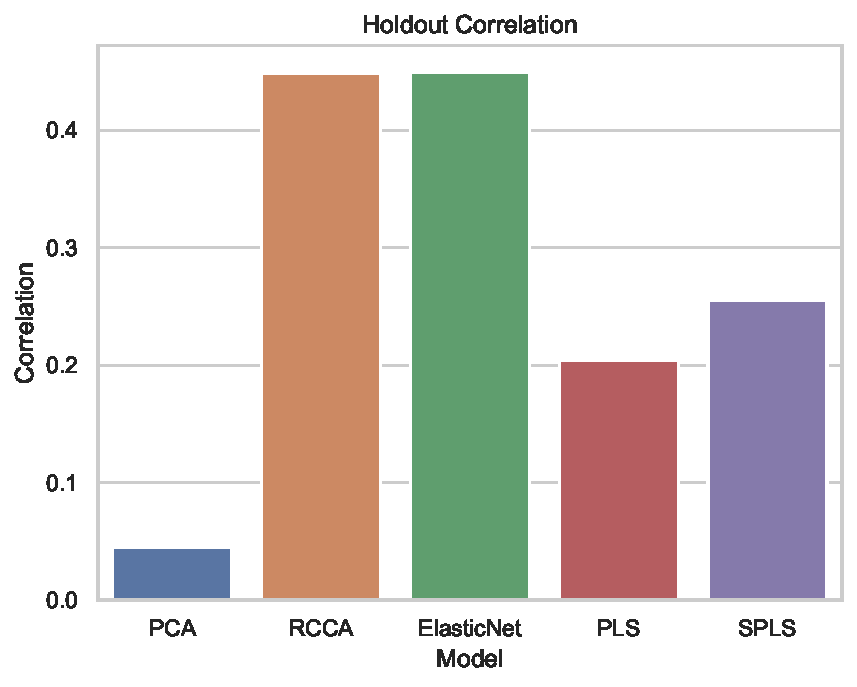
\includegraphics[width=0.5\linewidth]{figures/regularization/hcp/holdout_correlations.pdf}
\caption{Out-of-sample canonical correlations for each model.}\label{fig:performance}
\end{figure}

\subsubsection{Behaviour Weights and Loadings}

In this section, we plot the top 8 positive and negative non-imaging weights and loadings for each model.
This is to illustrate some of the effects we have observed in the previous section.
PCA finds a mode of variation in the behavioural data that is positively correlated with psychiatric and life function tests and negatively correlated with a number of emotion and personality tests.
The RCCA and ElasticNet models find a mode of variation in the behavioural data that is negatively correlated with the Line Orientation test and to a lesser extent smoking and positively correlated with a number of other cognitive tests.
The PLS model finds a mode of variation in the behavioural data that is somewhat similar to the `good-bad' mode in \cite{smith2015positive} with a positive correlation with agreeableness, vocabulary tests, and feelings about ones life and a strong negative correlation with smoking, rule-breaking, and antisocial personality traits.
The SPLS mode is similar but selects out the rule-breaking and antisocial personality traits in favour of the vocabulary tests and smoking.

\begin{figure}
\centering
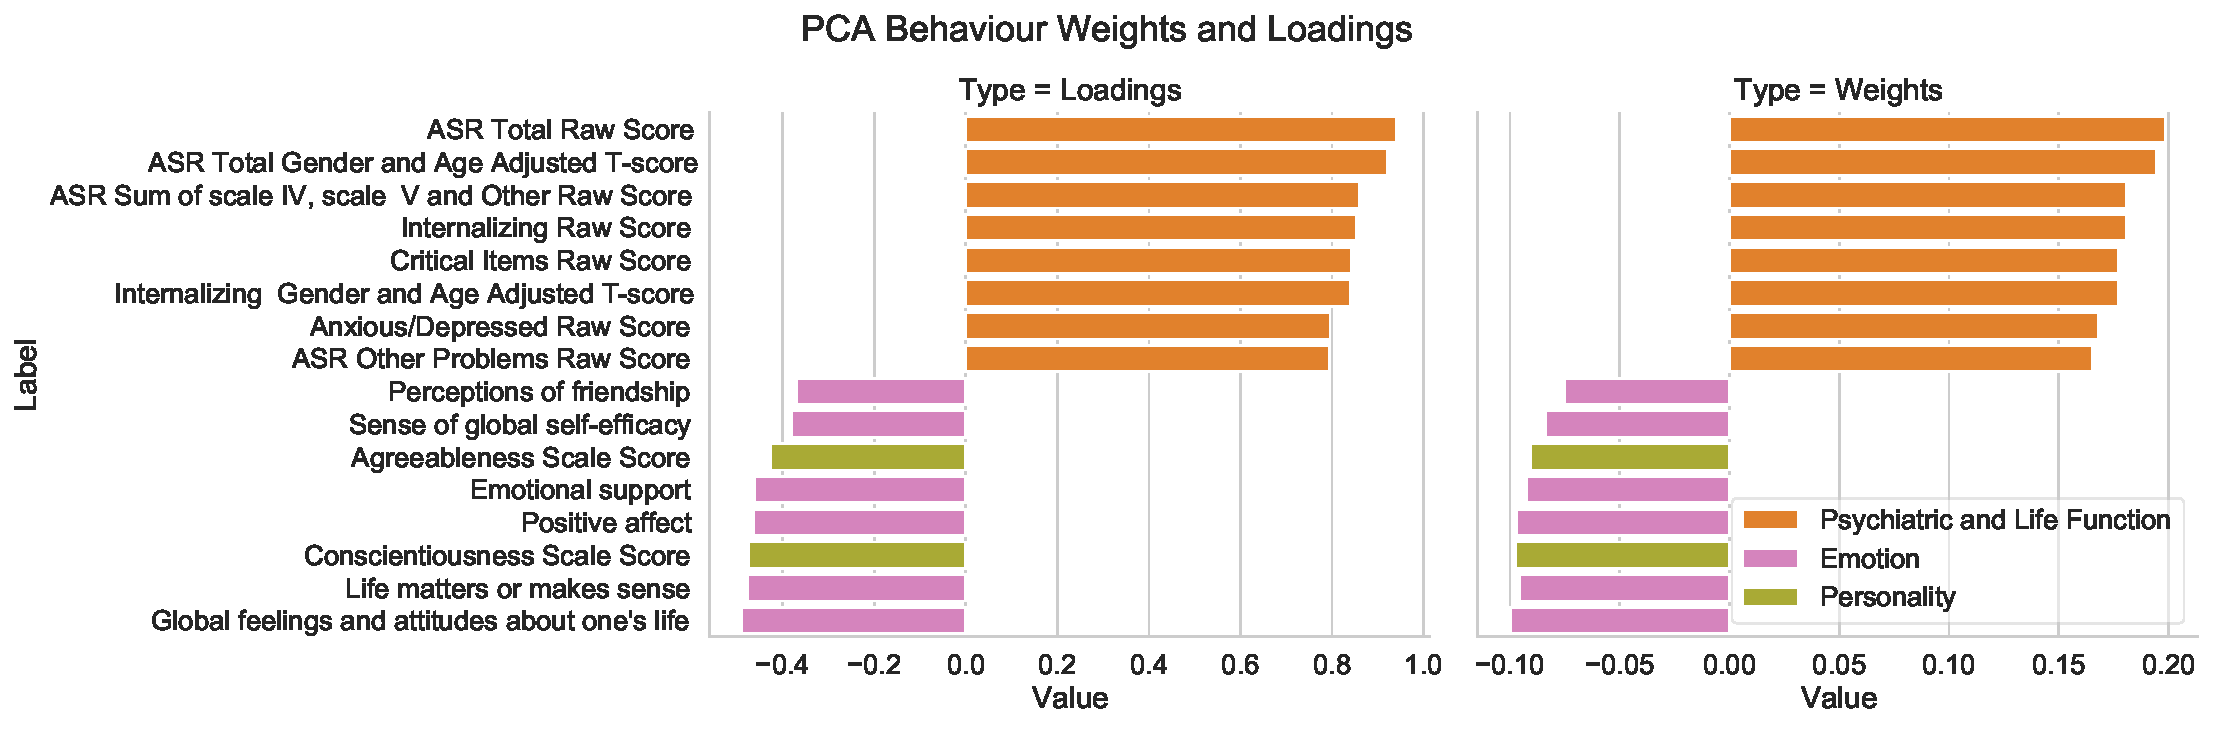
\includegraphics[width=0.8\linewidth]{figures/regularization/hcp/PCA behaviour weights and loadings.pdf}
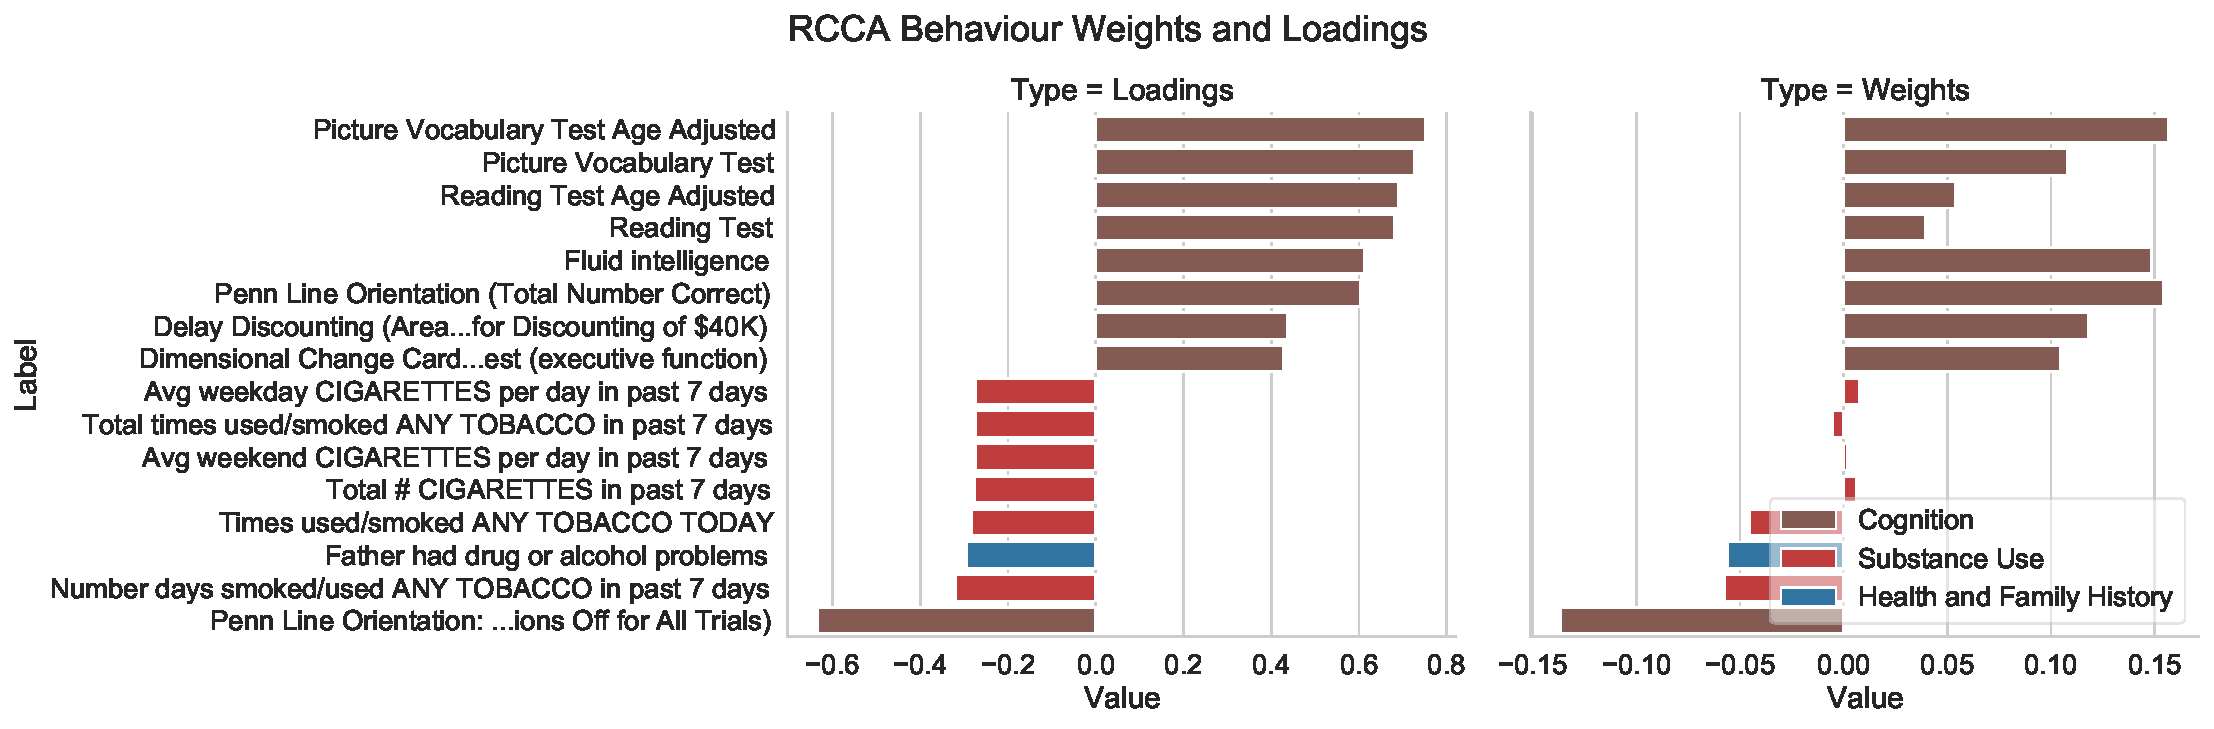
\includegraphics[width=0.8\linewidth]{figures/regularization/hcp/RCCA behaviour weights and loadings.pdf}
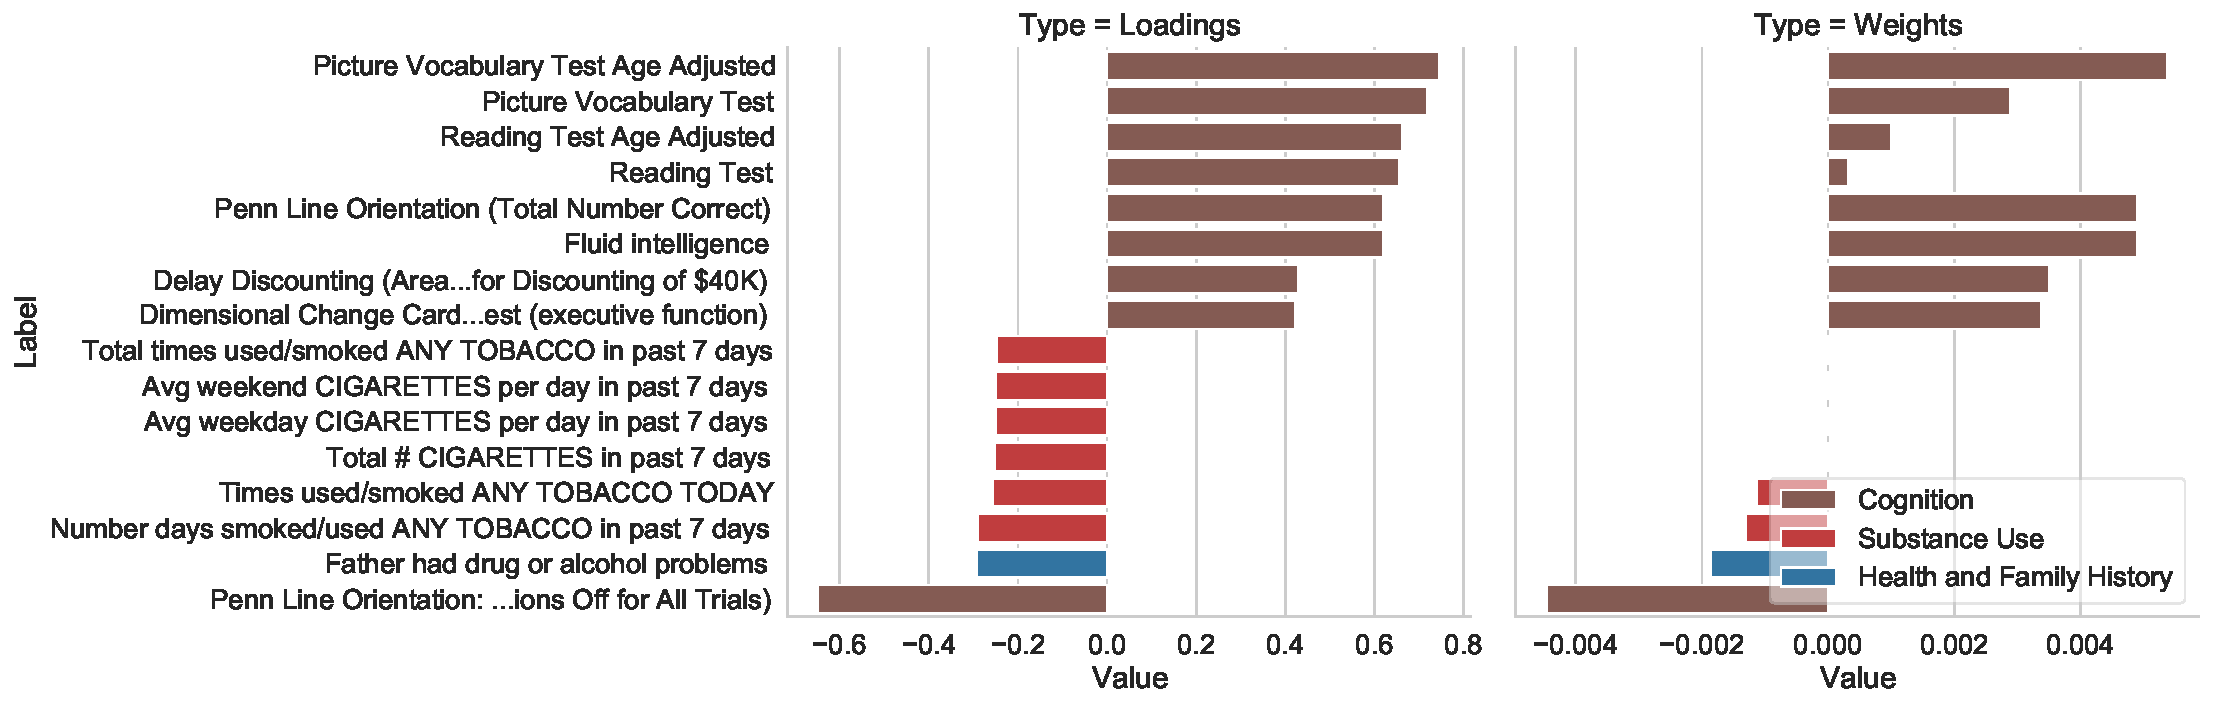
\includegraphics[width=0.8\linewidth]{figures/regularization/hcp/ElasticNet behaviour weights and loadings.pdf}
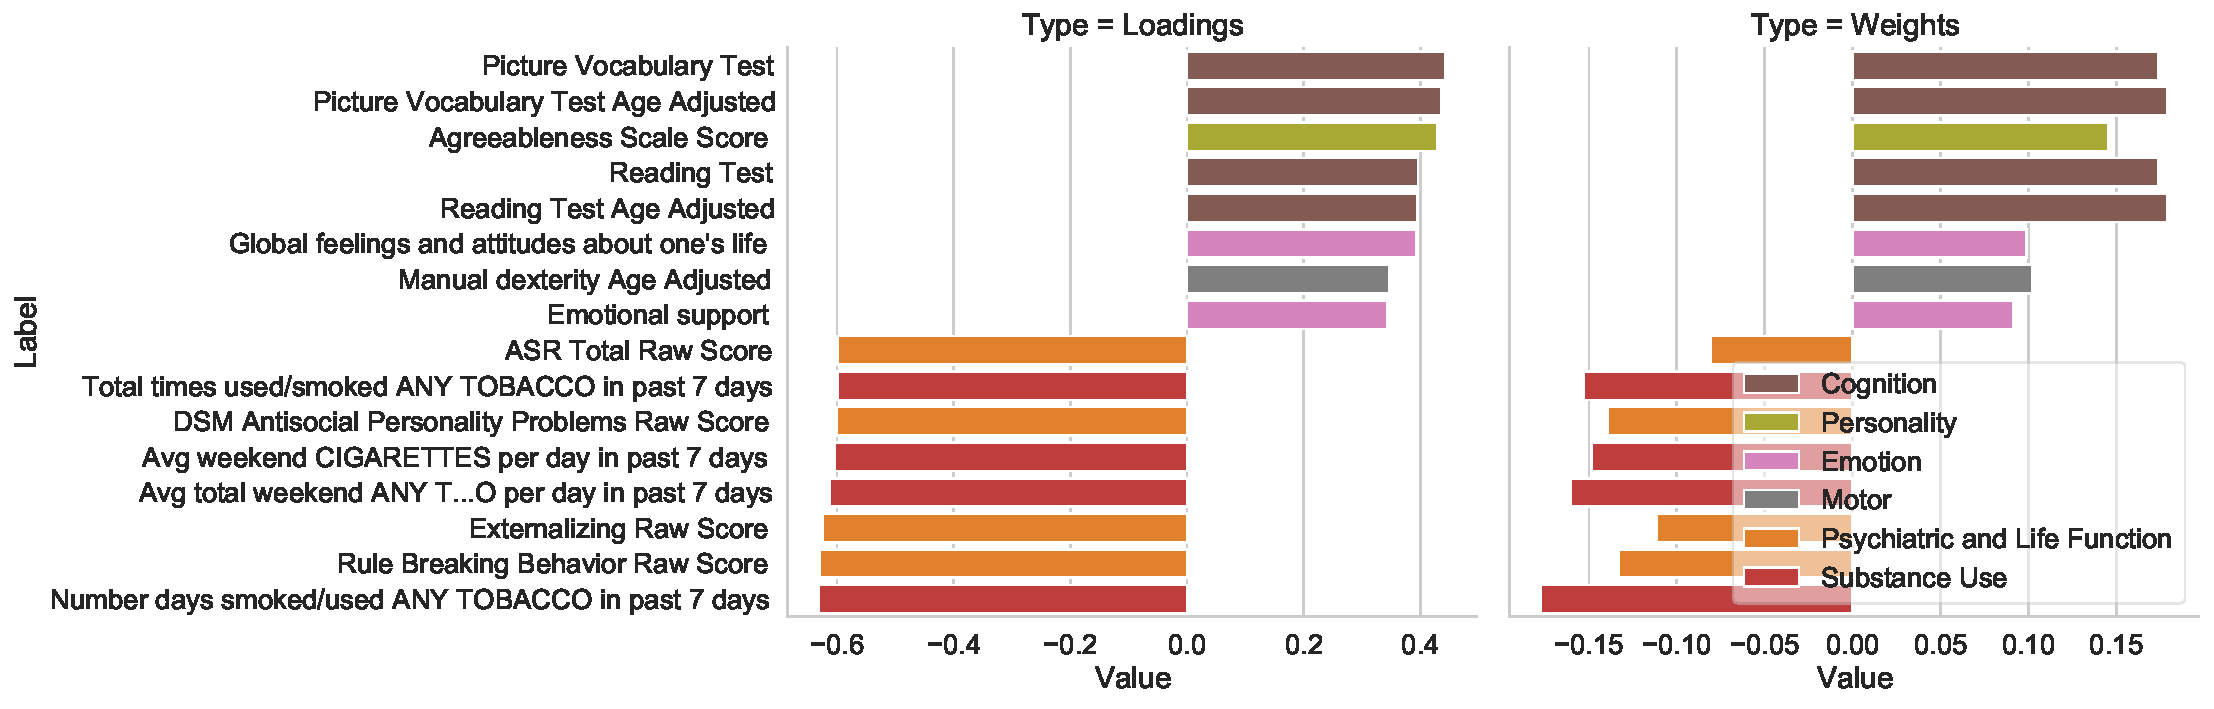
\includegraphics[width=0.8\linewidth]{figures/regularization/hcp/PLS behaviour weights and loadings.pdf}
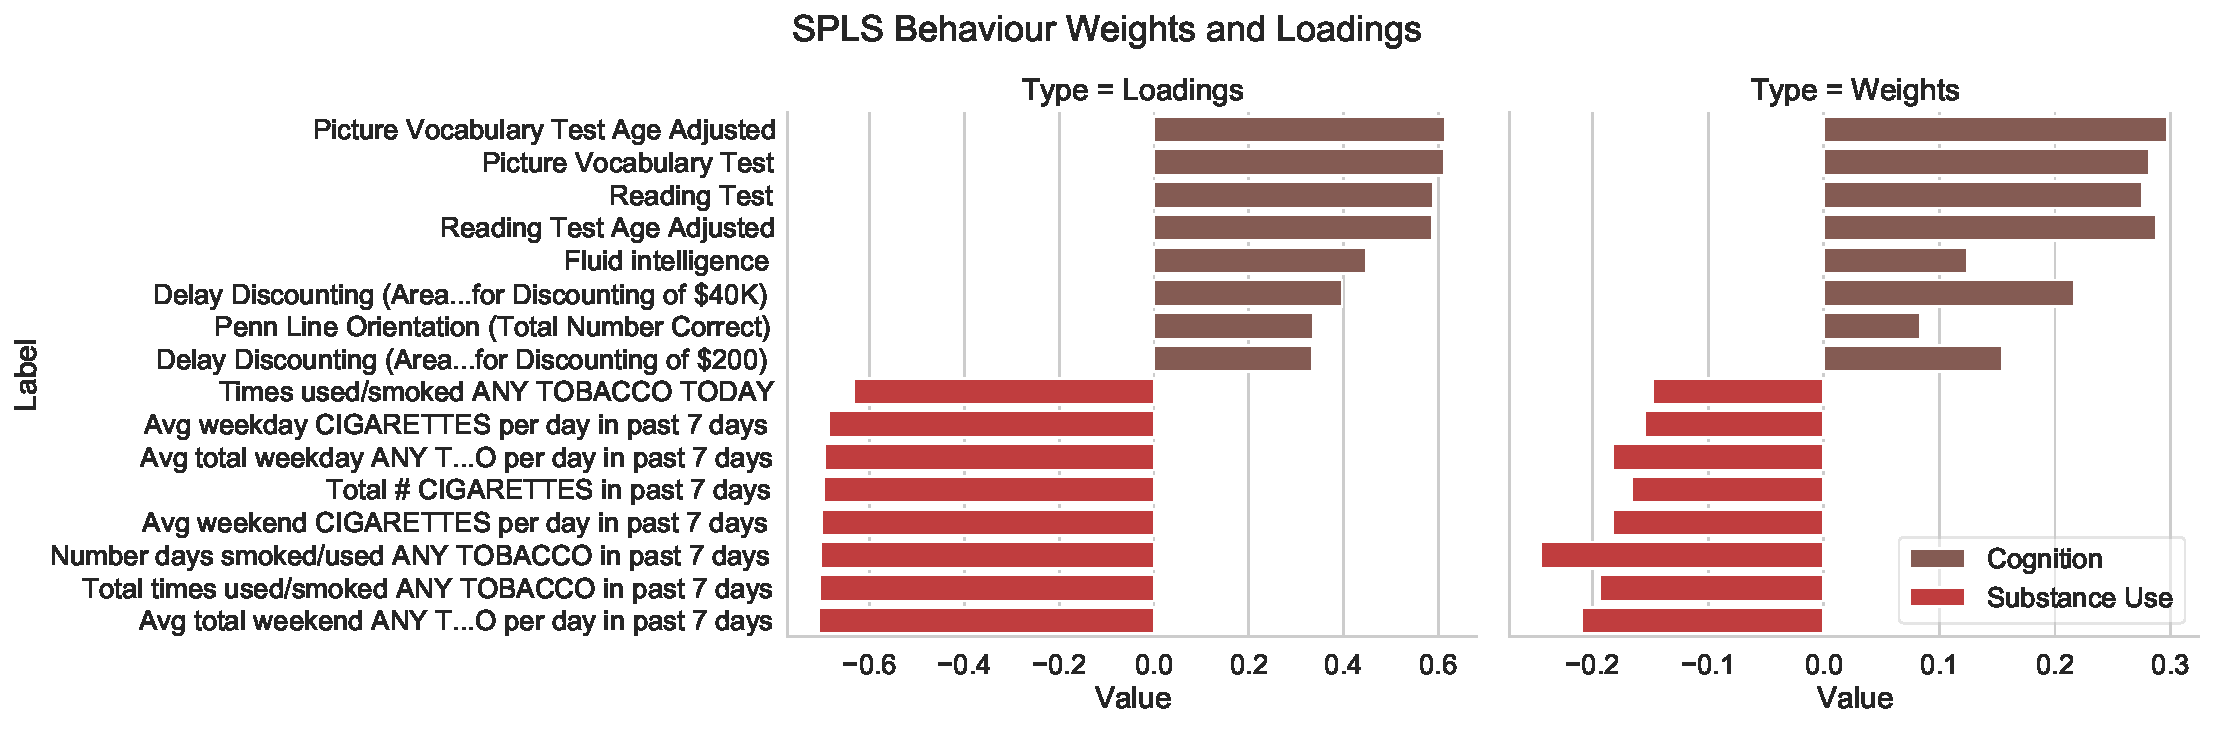
\includegraphics[width=0.8\linewidth]{figures/regularization/hcp/SPLS behaviour weights and loadings.pdf}
\caption{Top 8 positive and negative non-imaging loadings for each model}\label{fig:behaviour}
\end{figure}

\subsubsection{Connectivity Weights}
\begin{figure}
\centering
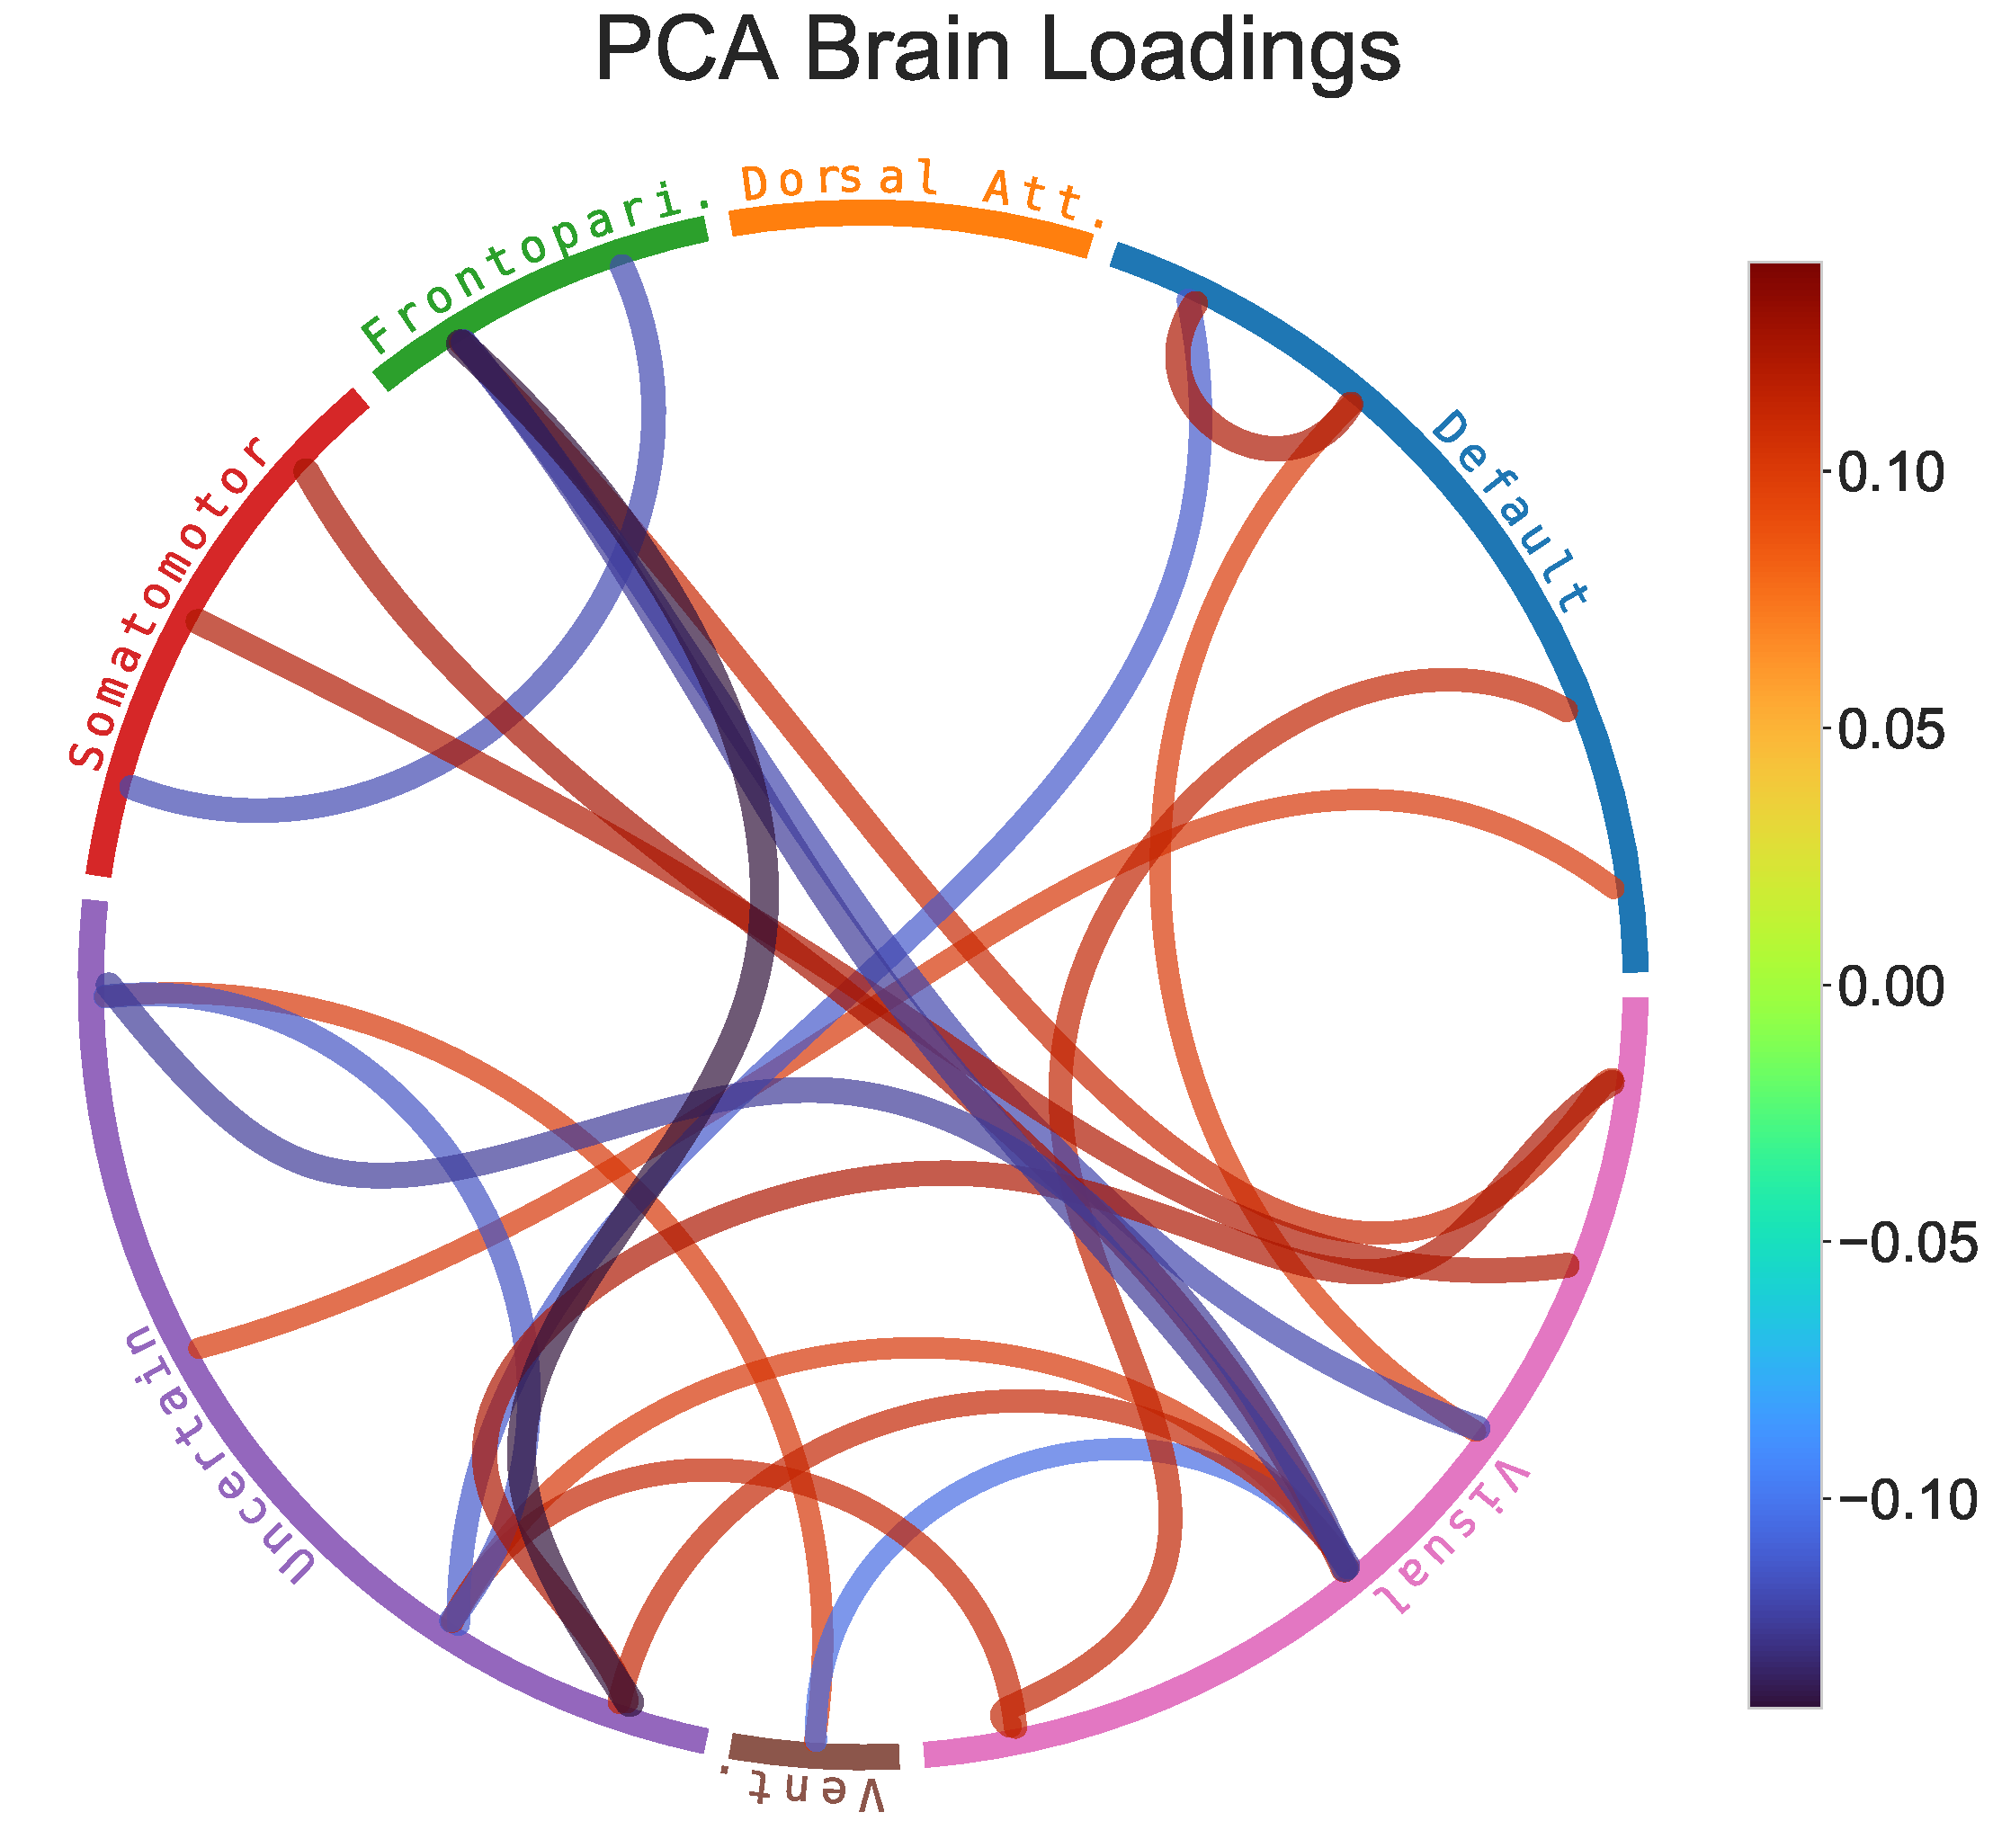
\includegraphics[width=0.49\linewidth]{figures/regularization/hcp/PCA brain weights.pdf}
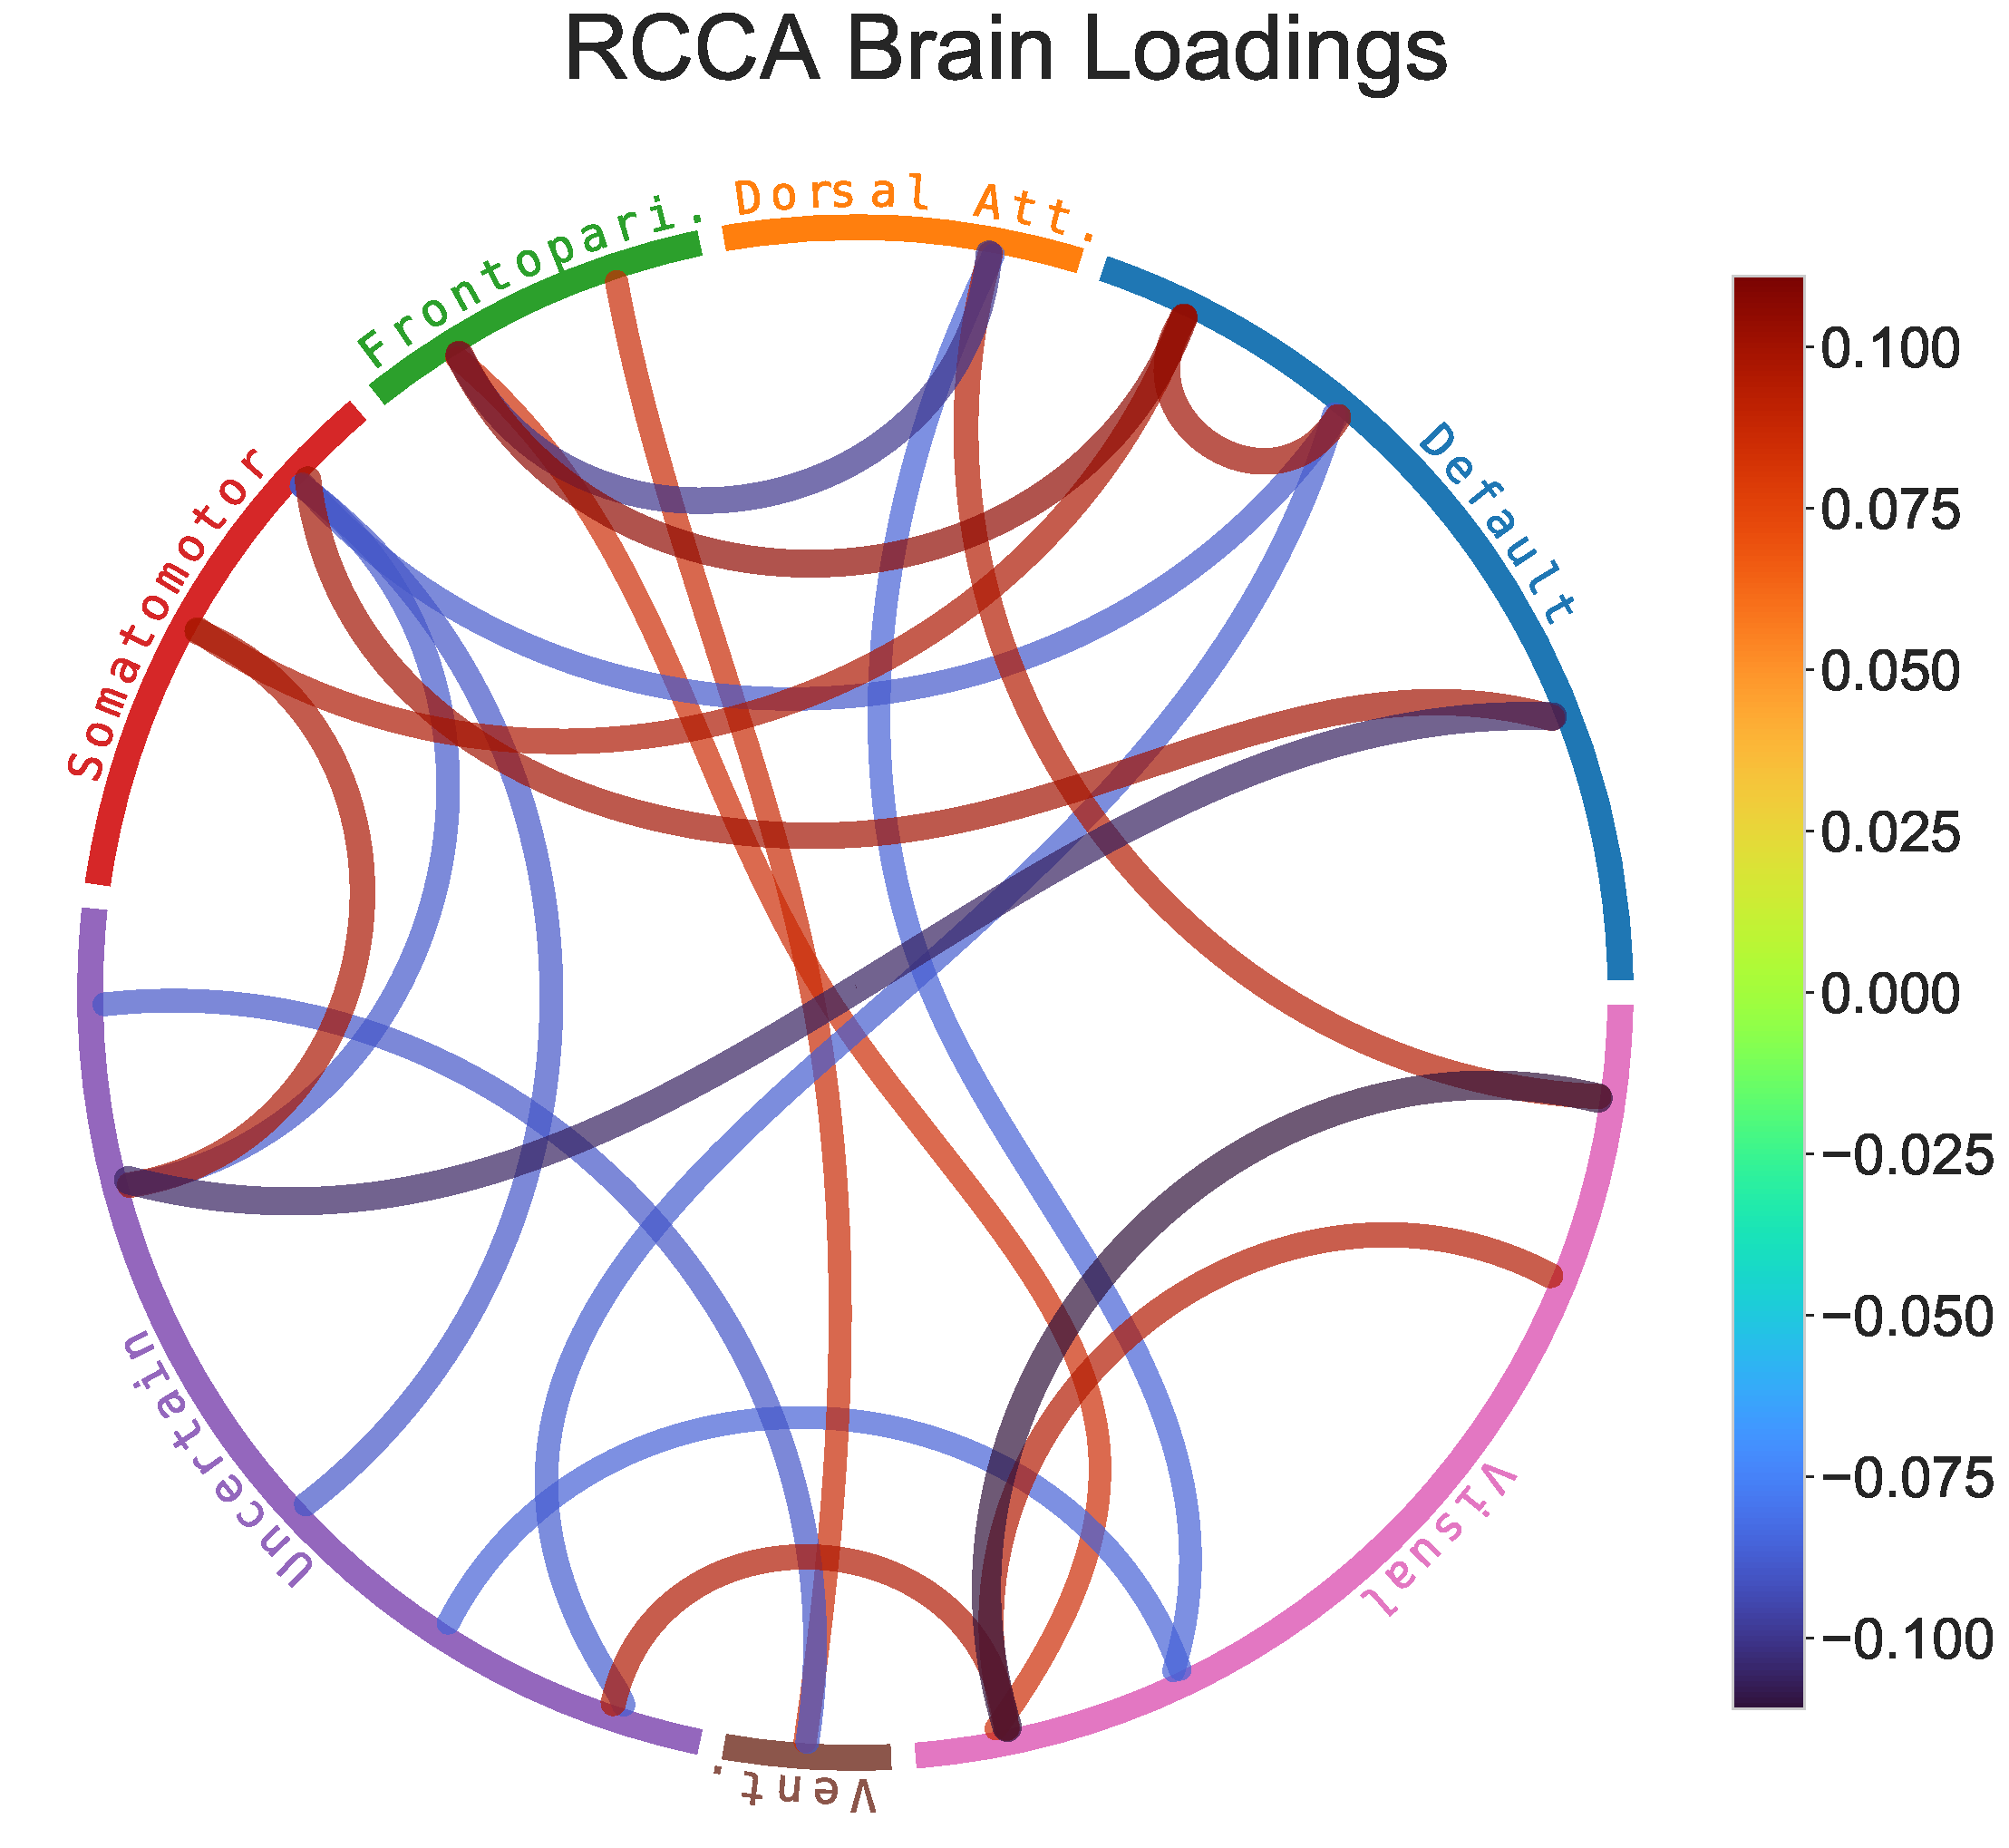
\includegraphics[width=0.49\linewidth]{figures/regularization/hcp/RCCA brain weights.pdf}
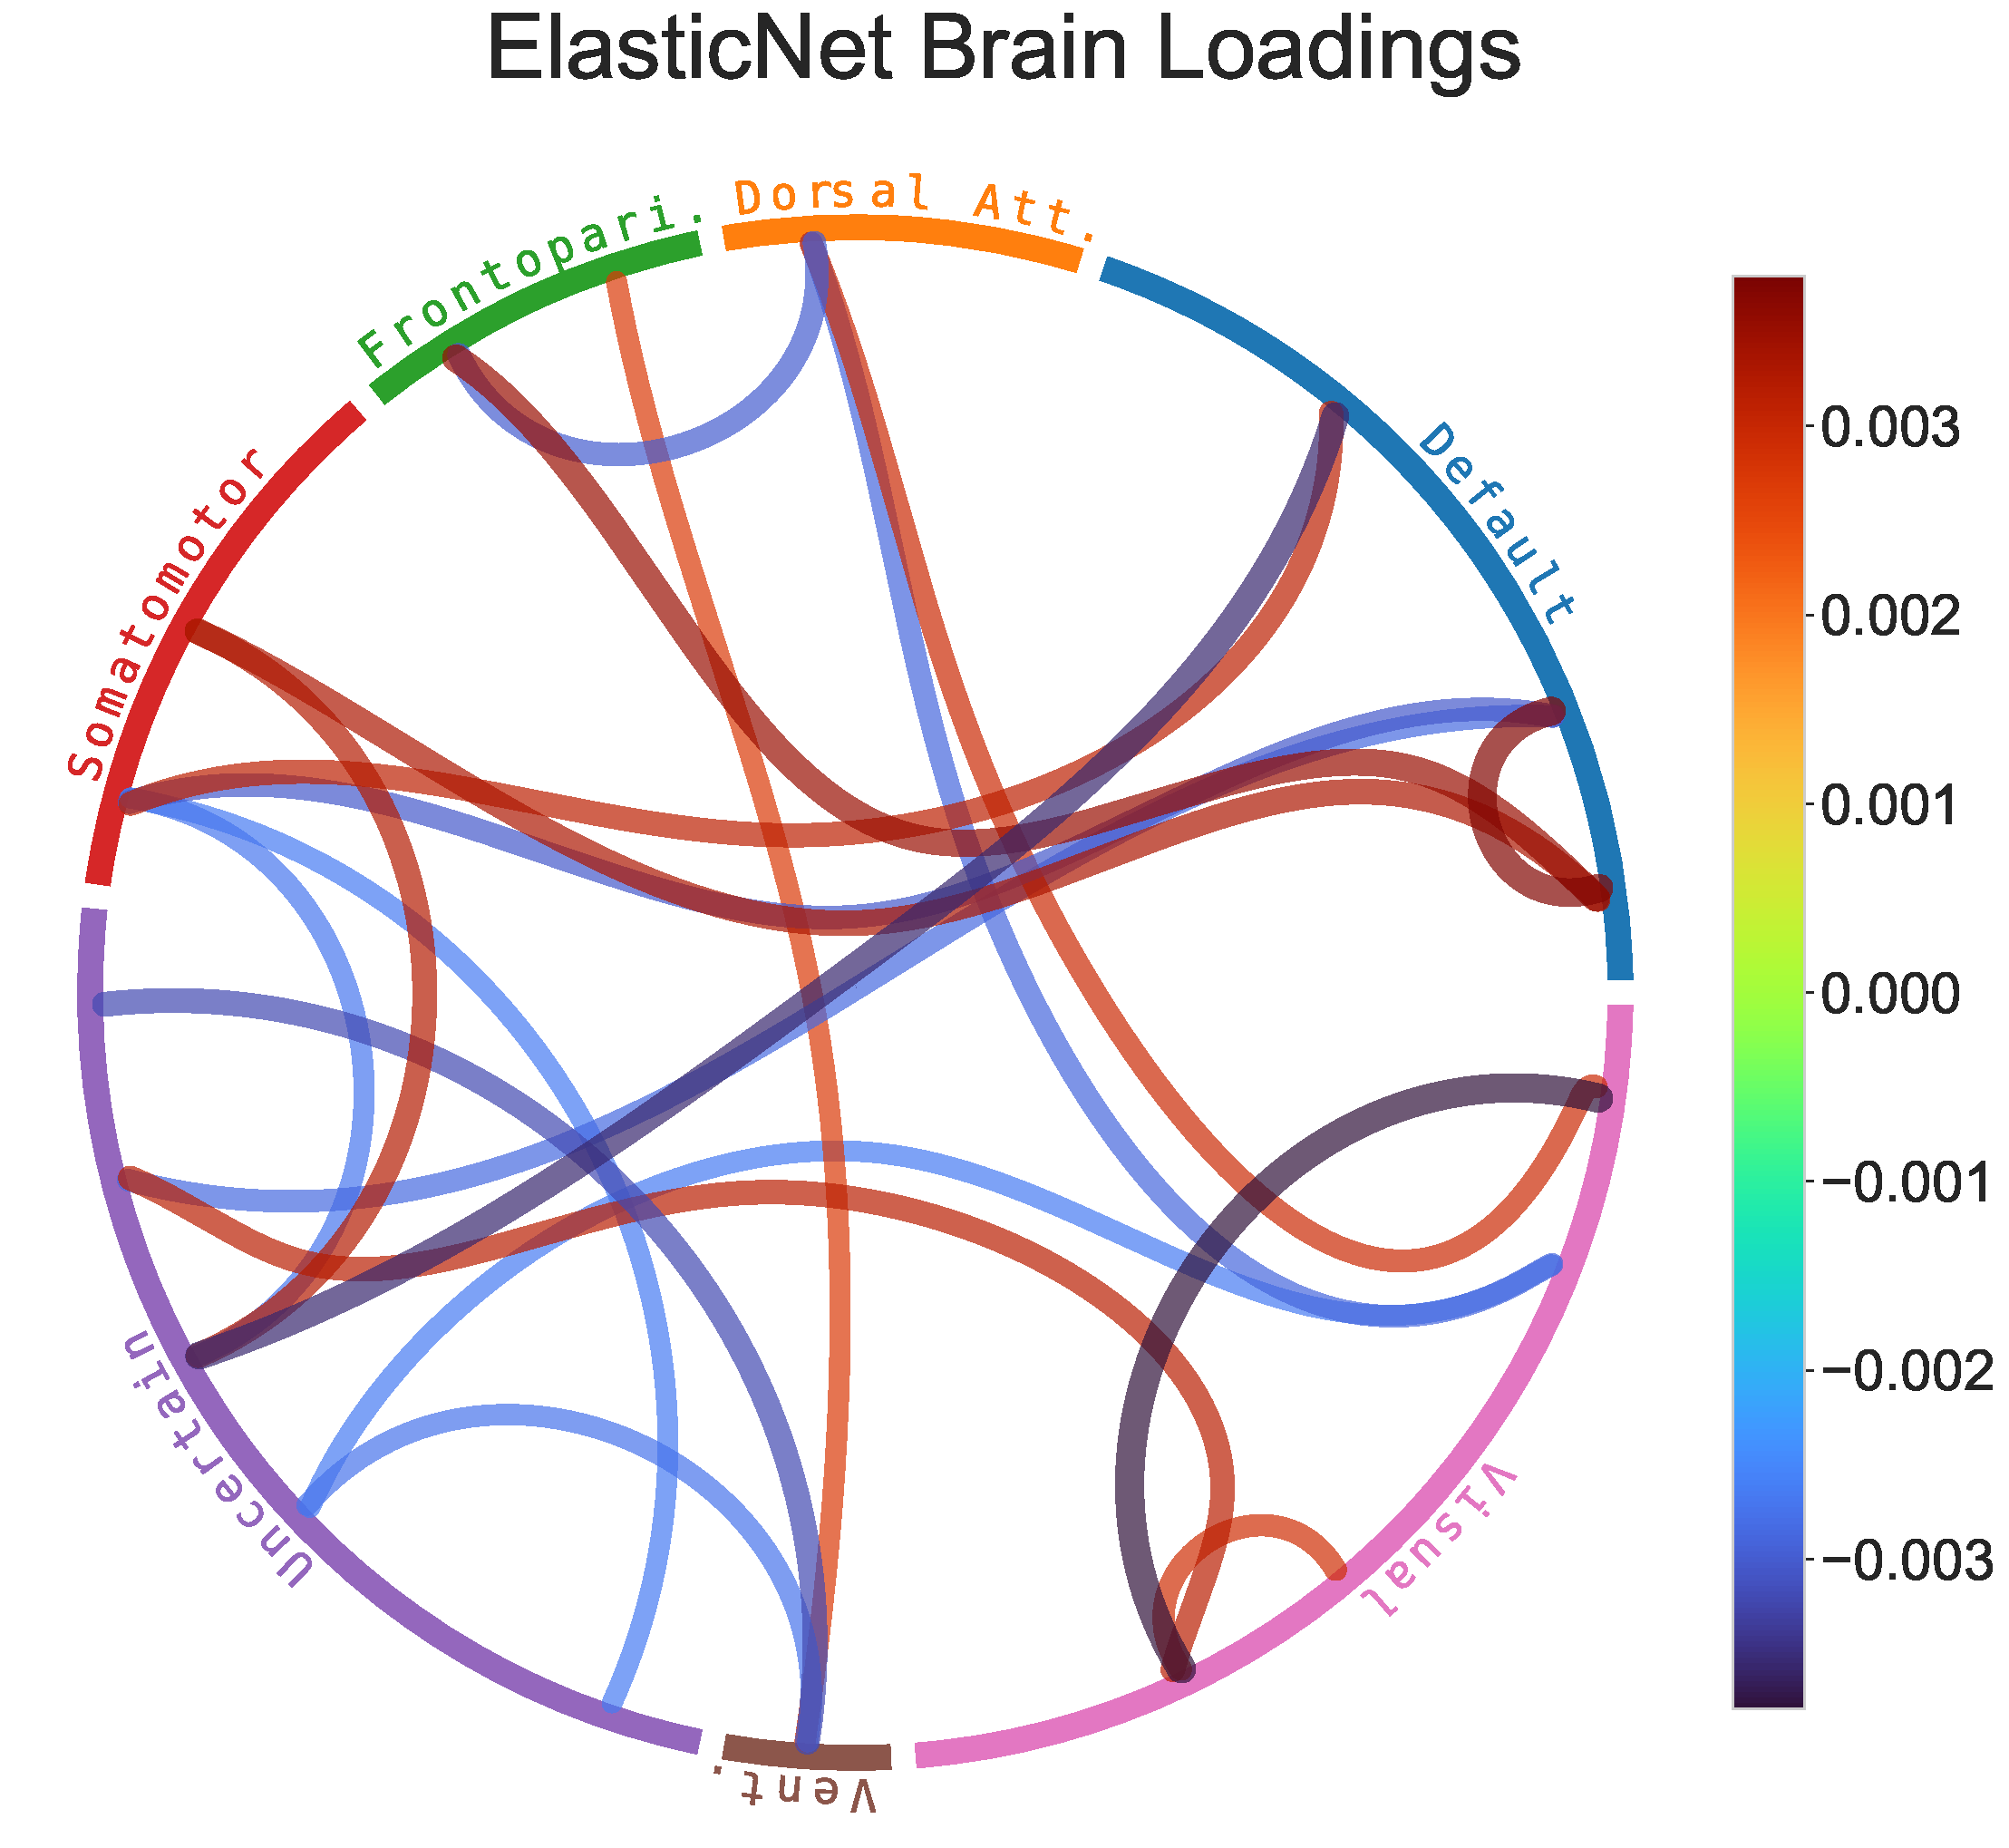
\includegraphics[width=0.49\linewidth]{figures/regularization/hcp/ElasticNet brain weights.pdf}
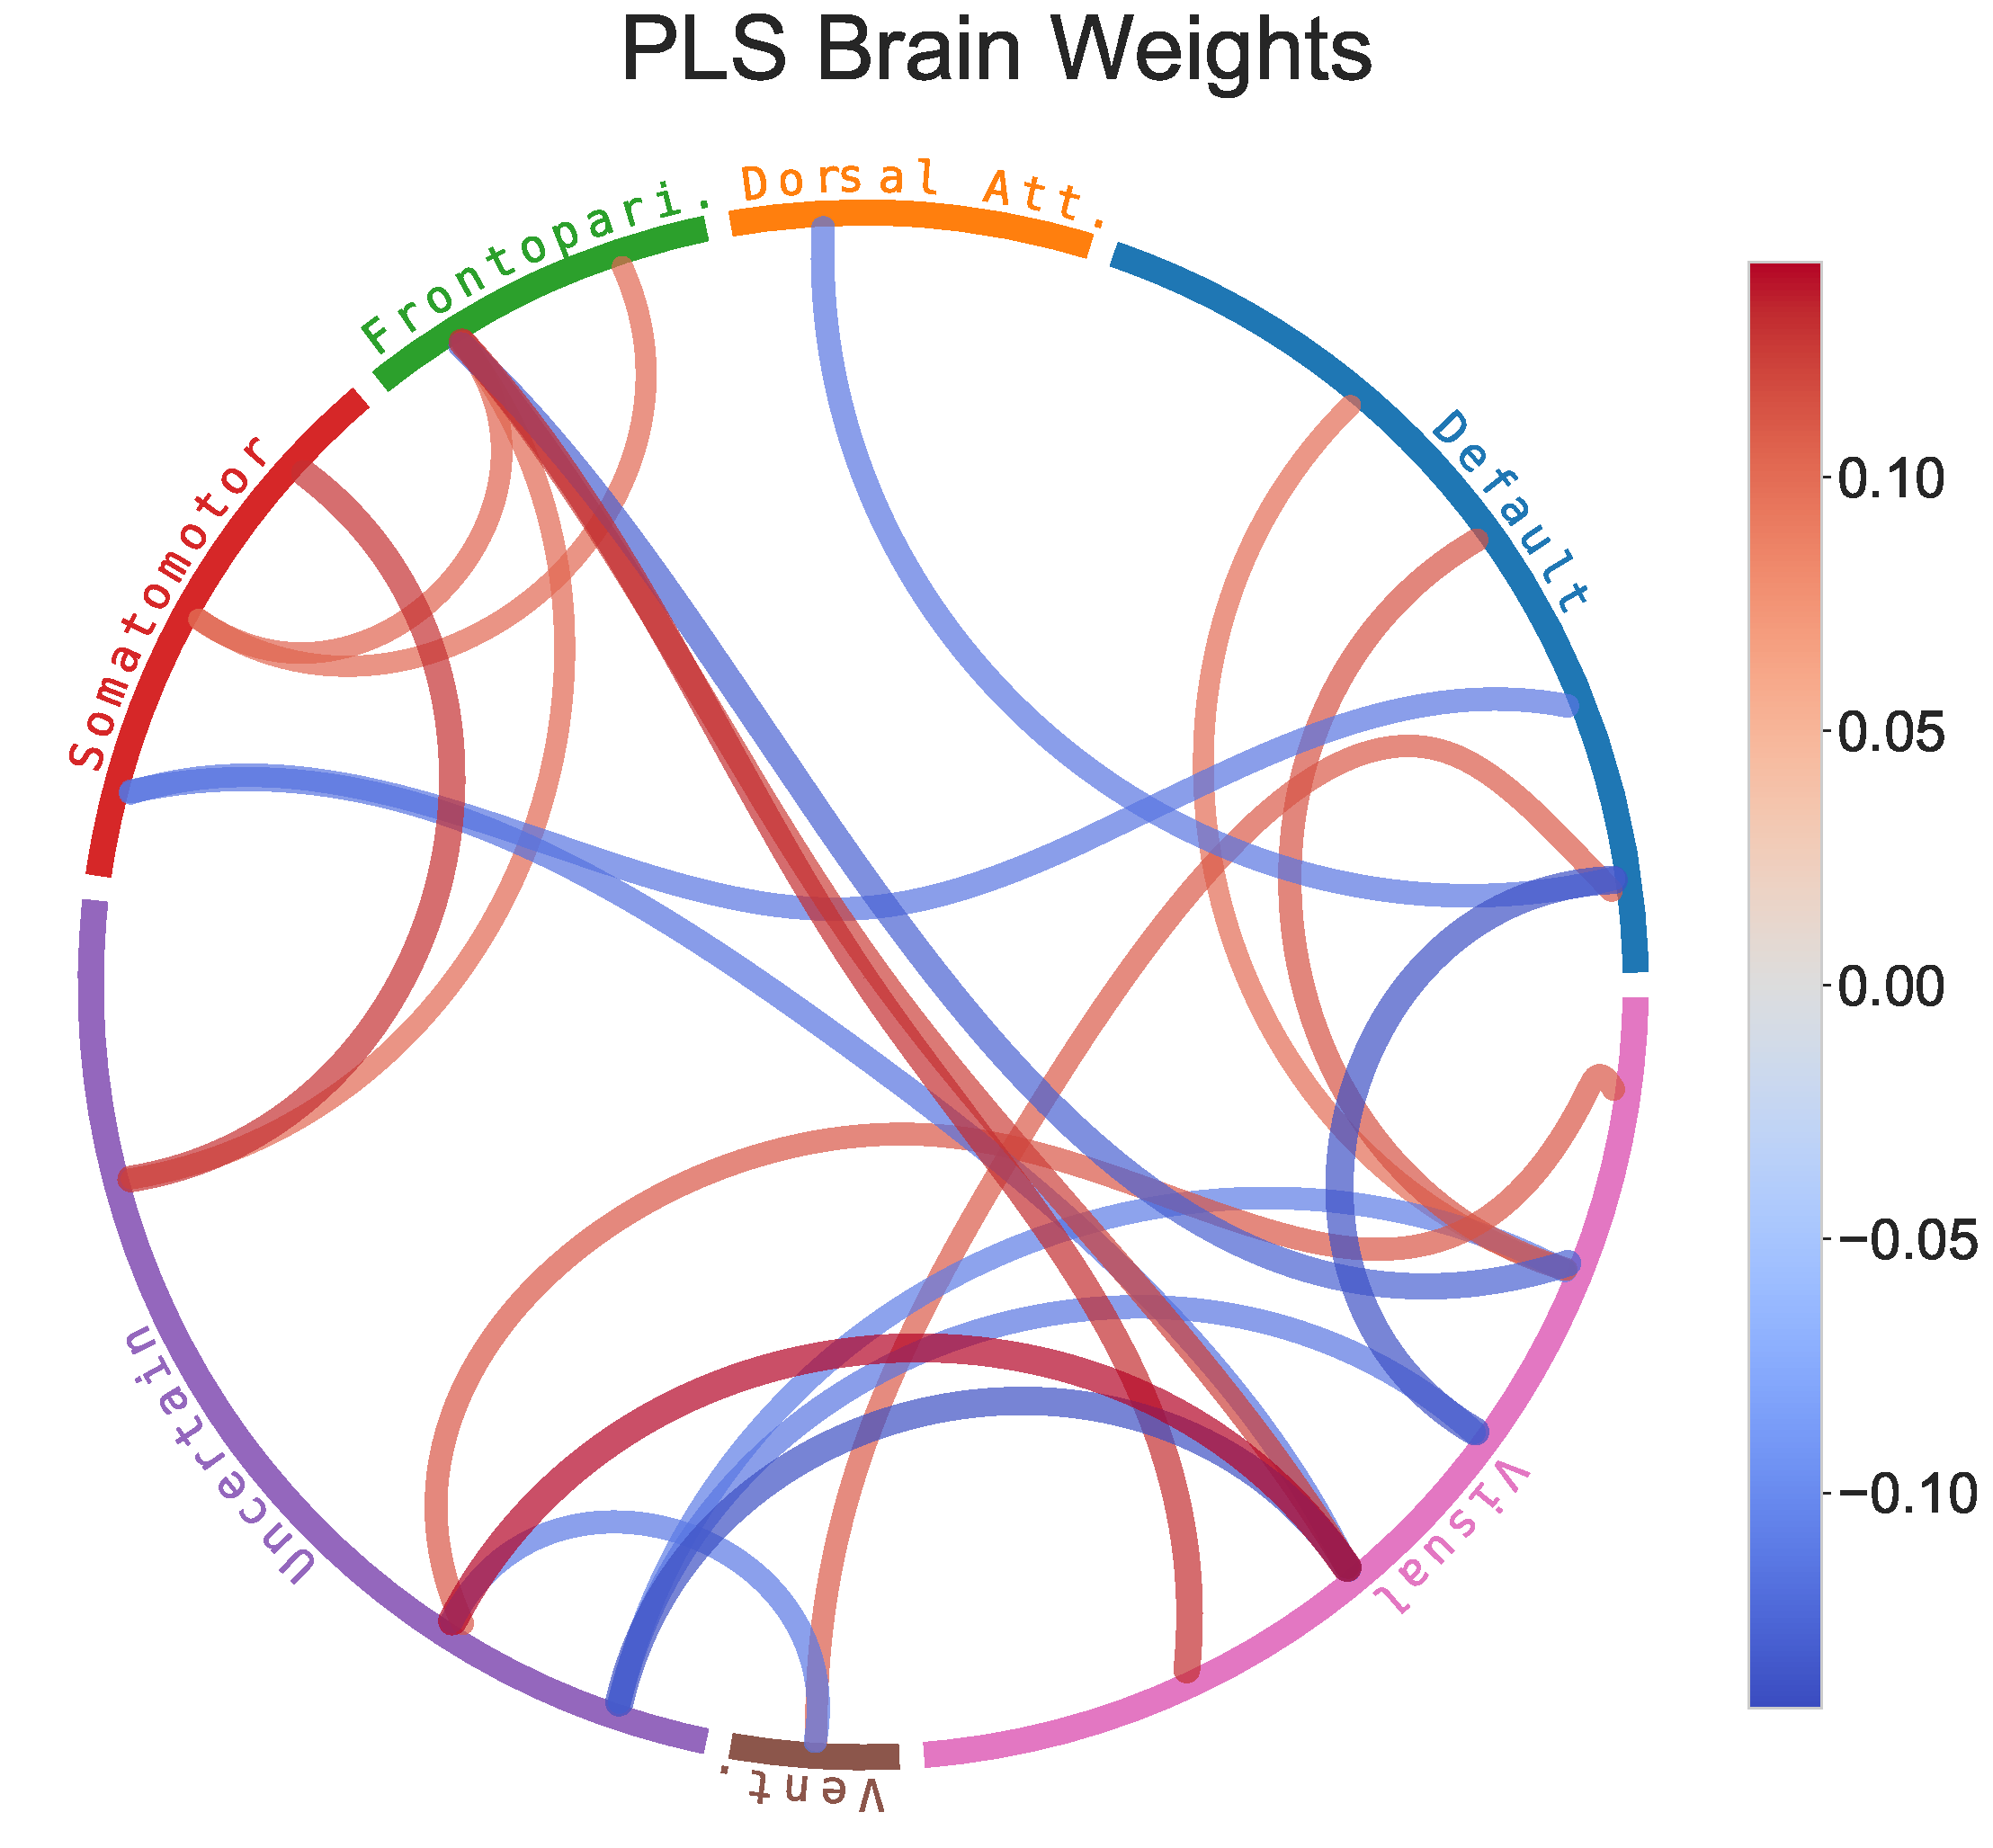
\includegraphics[width=0.49\linewidth]{figures/regularization/hcp/PLS brain weights.pdf}
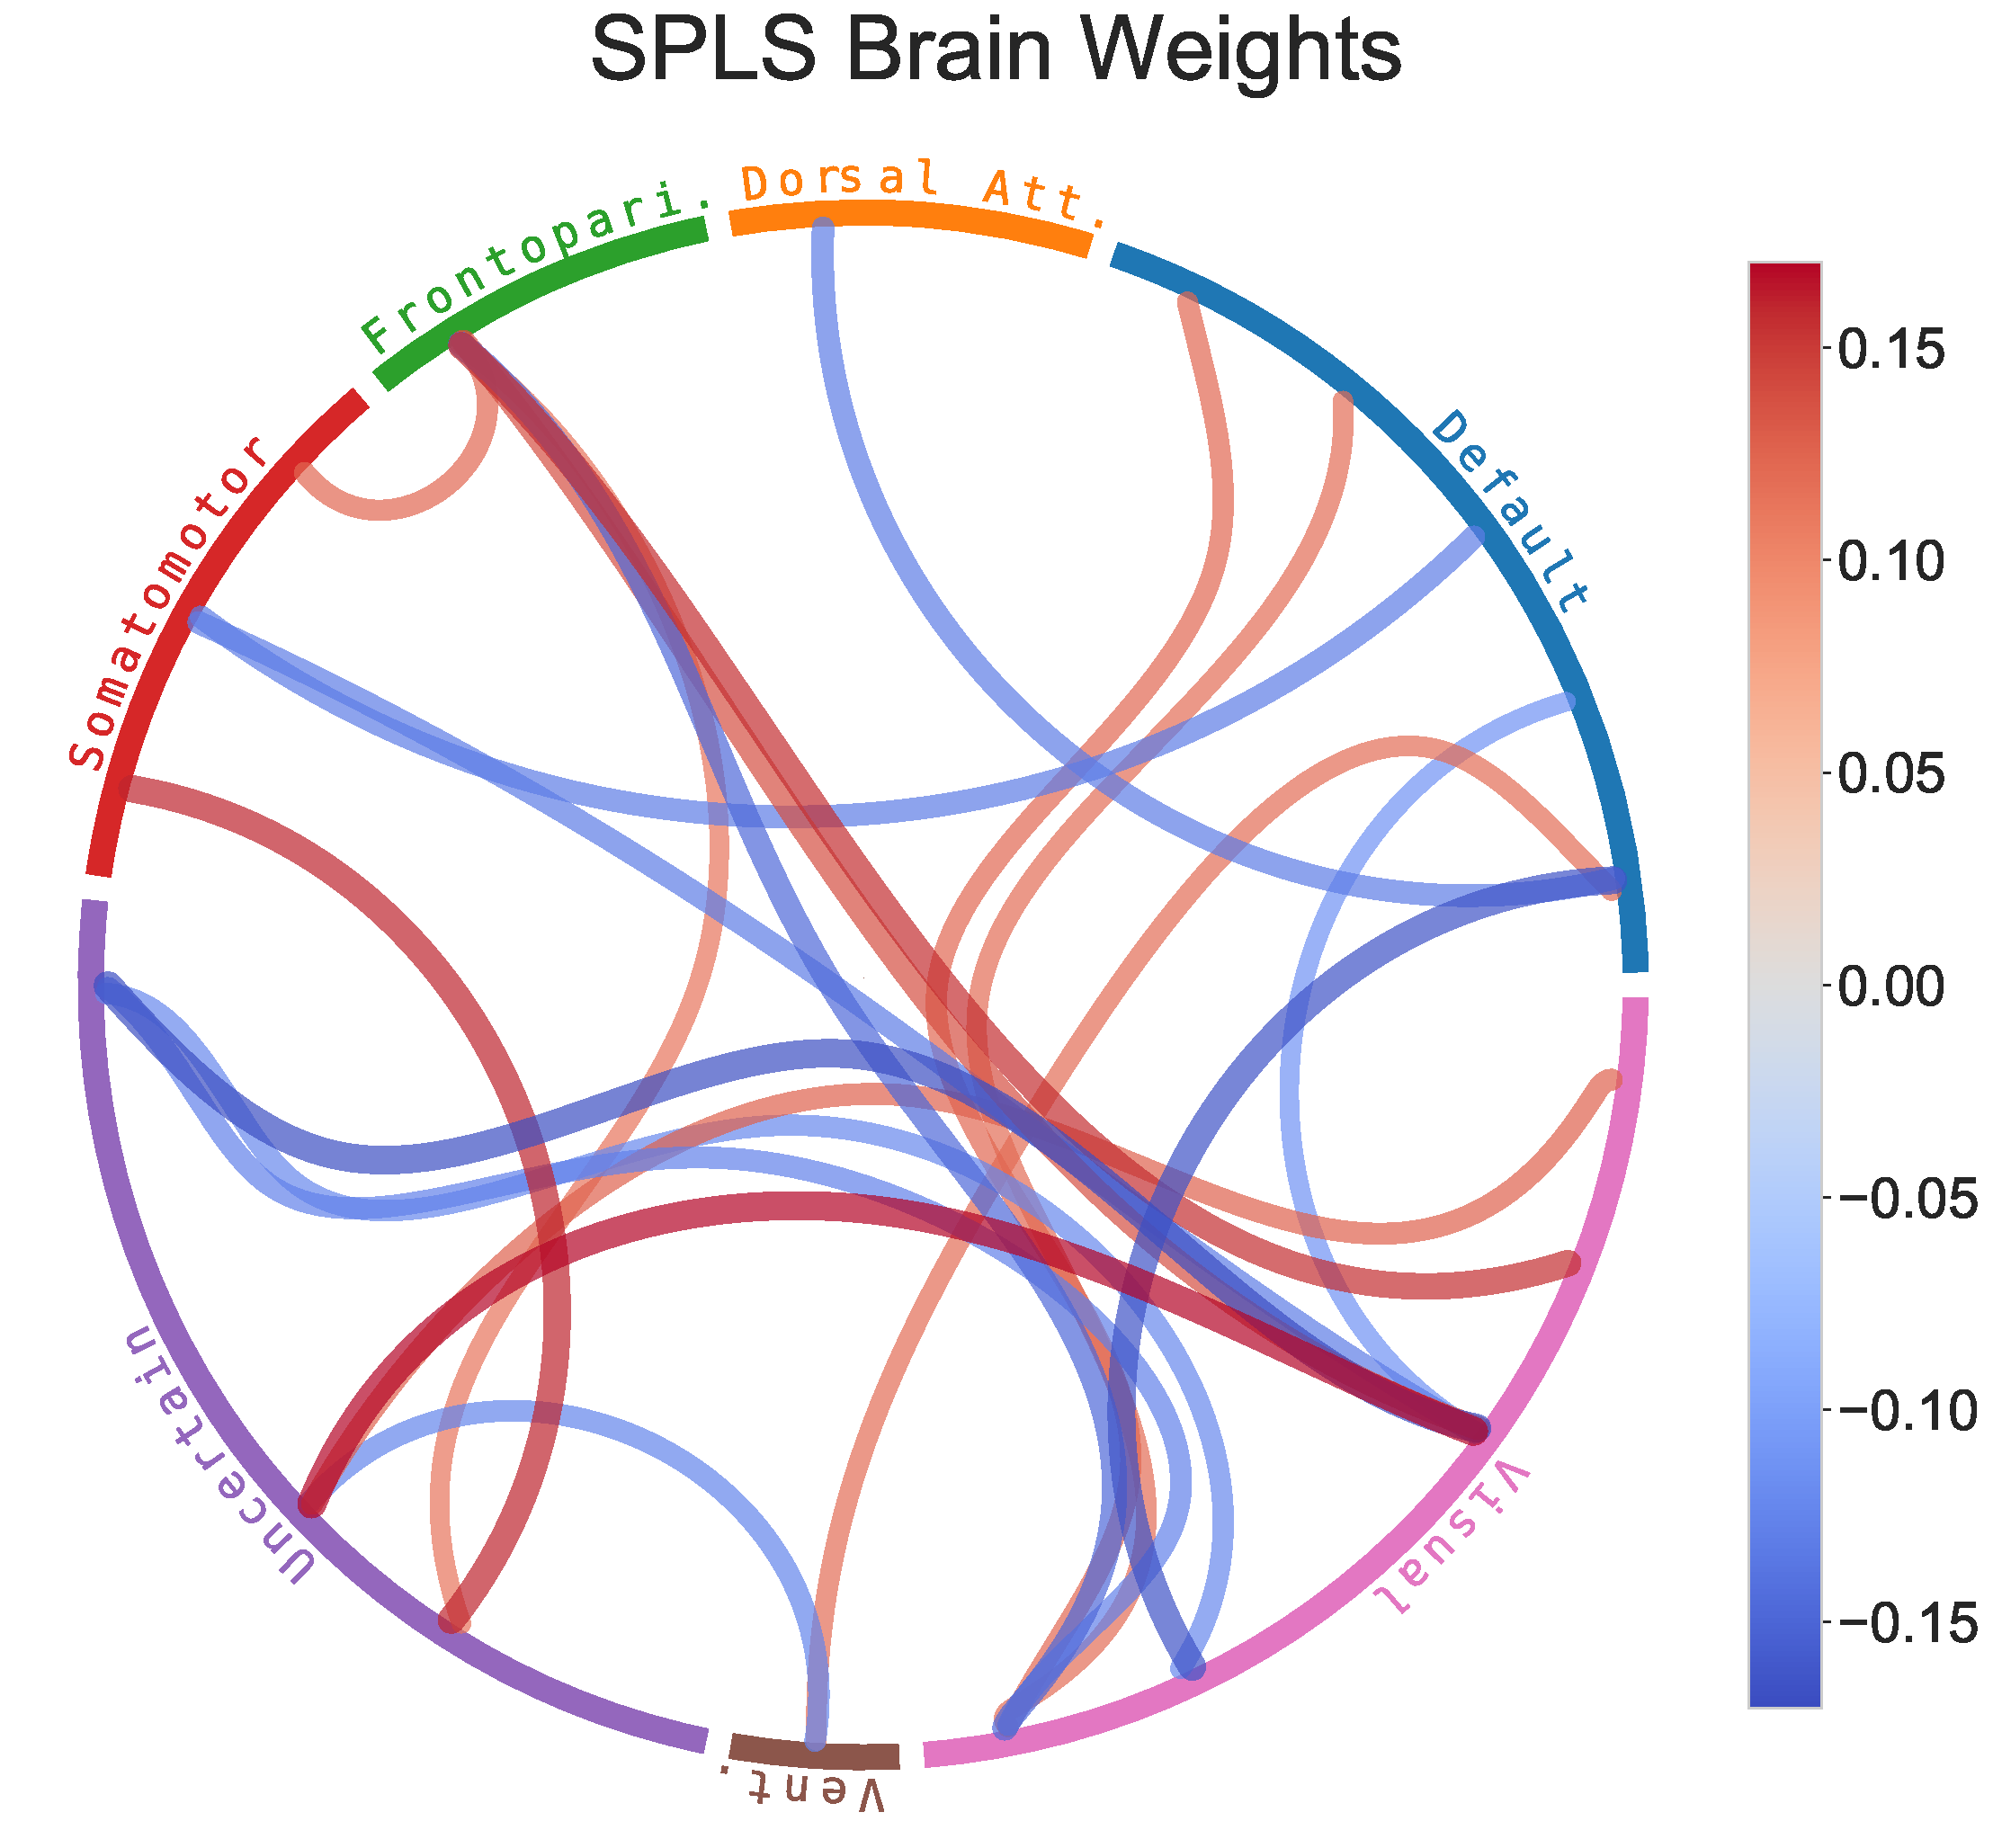
\includegraphics[width=0.49\linewidth]{figures/regularization/hcp/SPLS brain weights.pdf}
\caption{}\label{}
\end{figure}

\subsubsection{Connectivity Loadings}
\begin{figure}
\centering
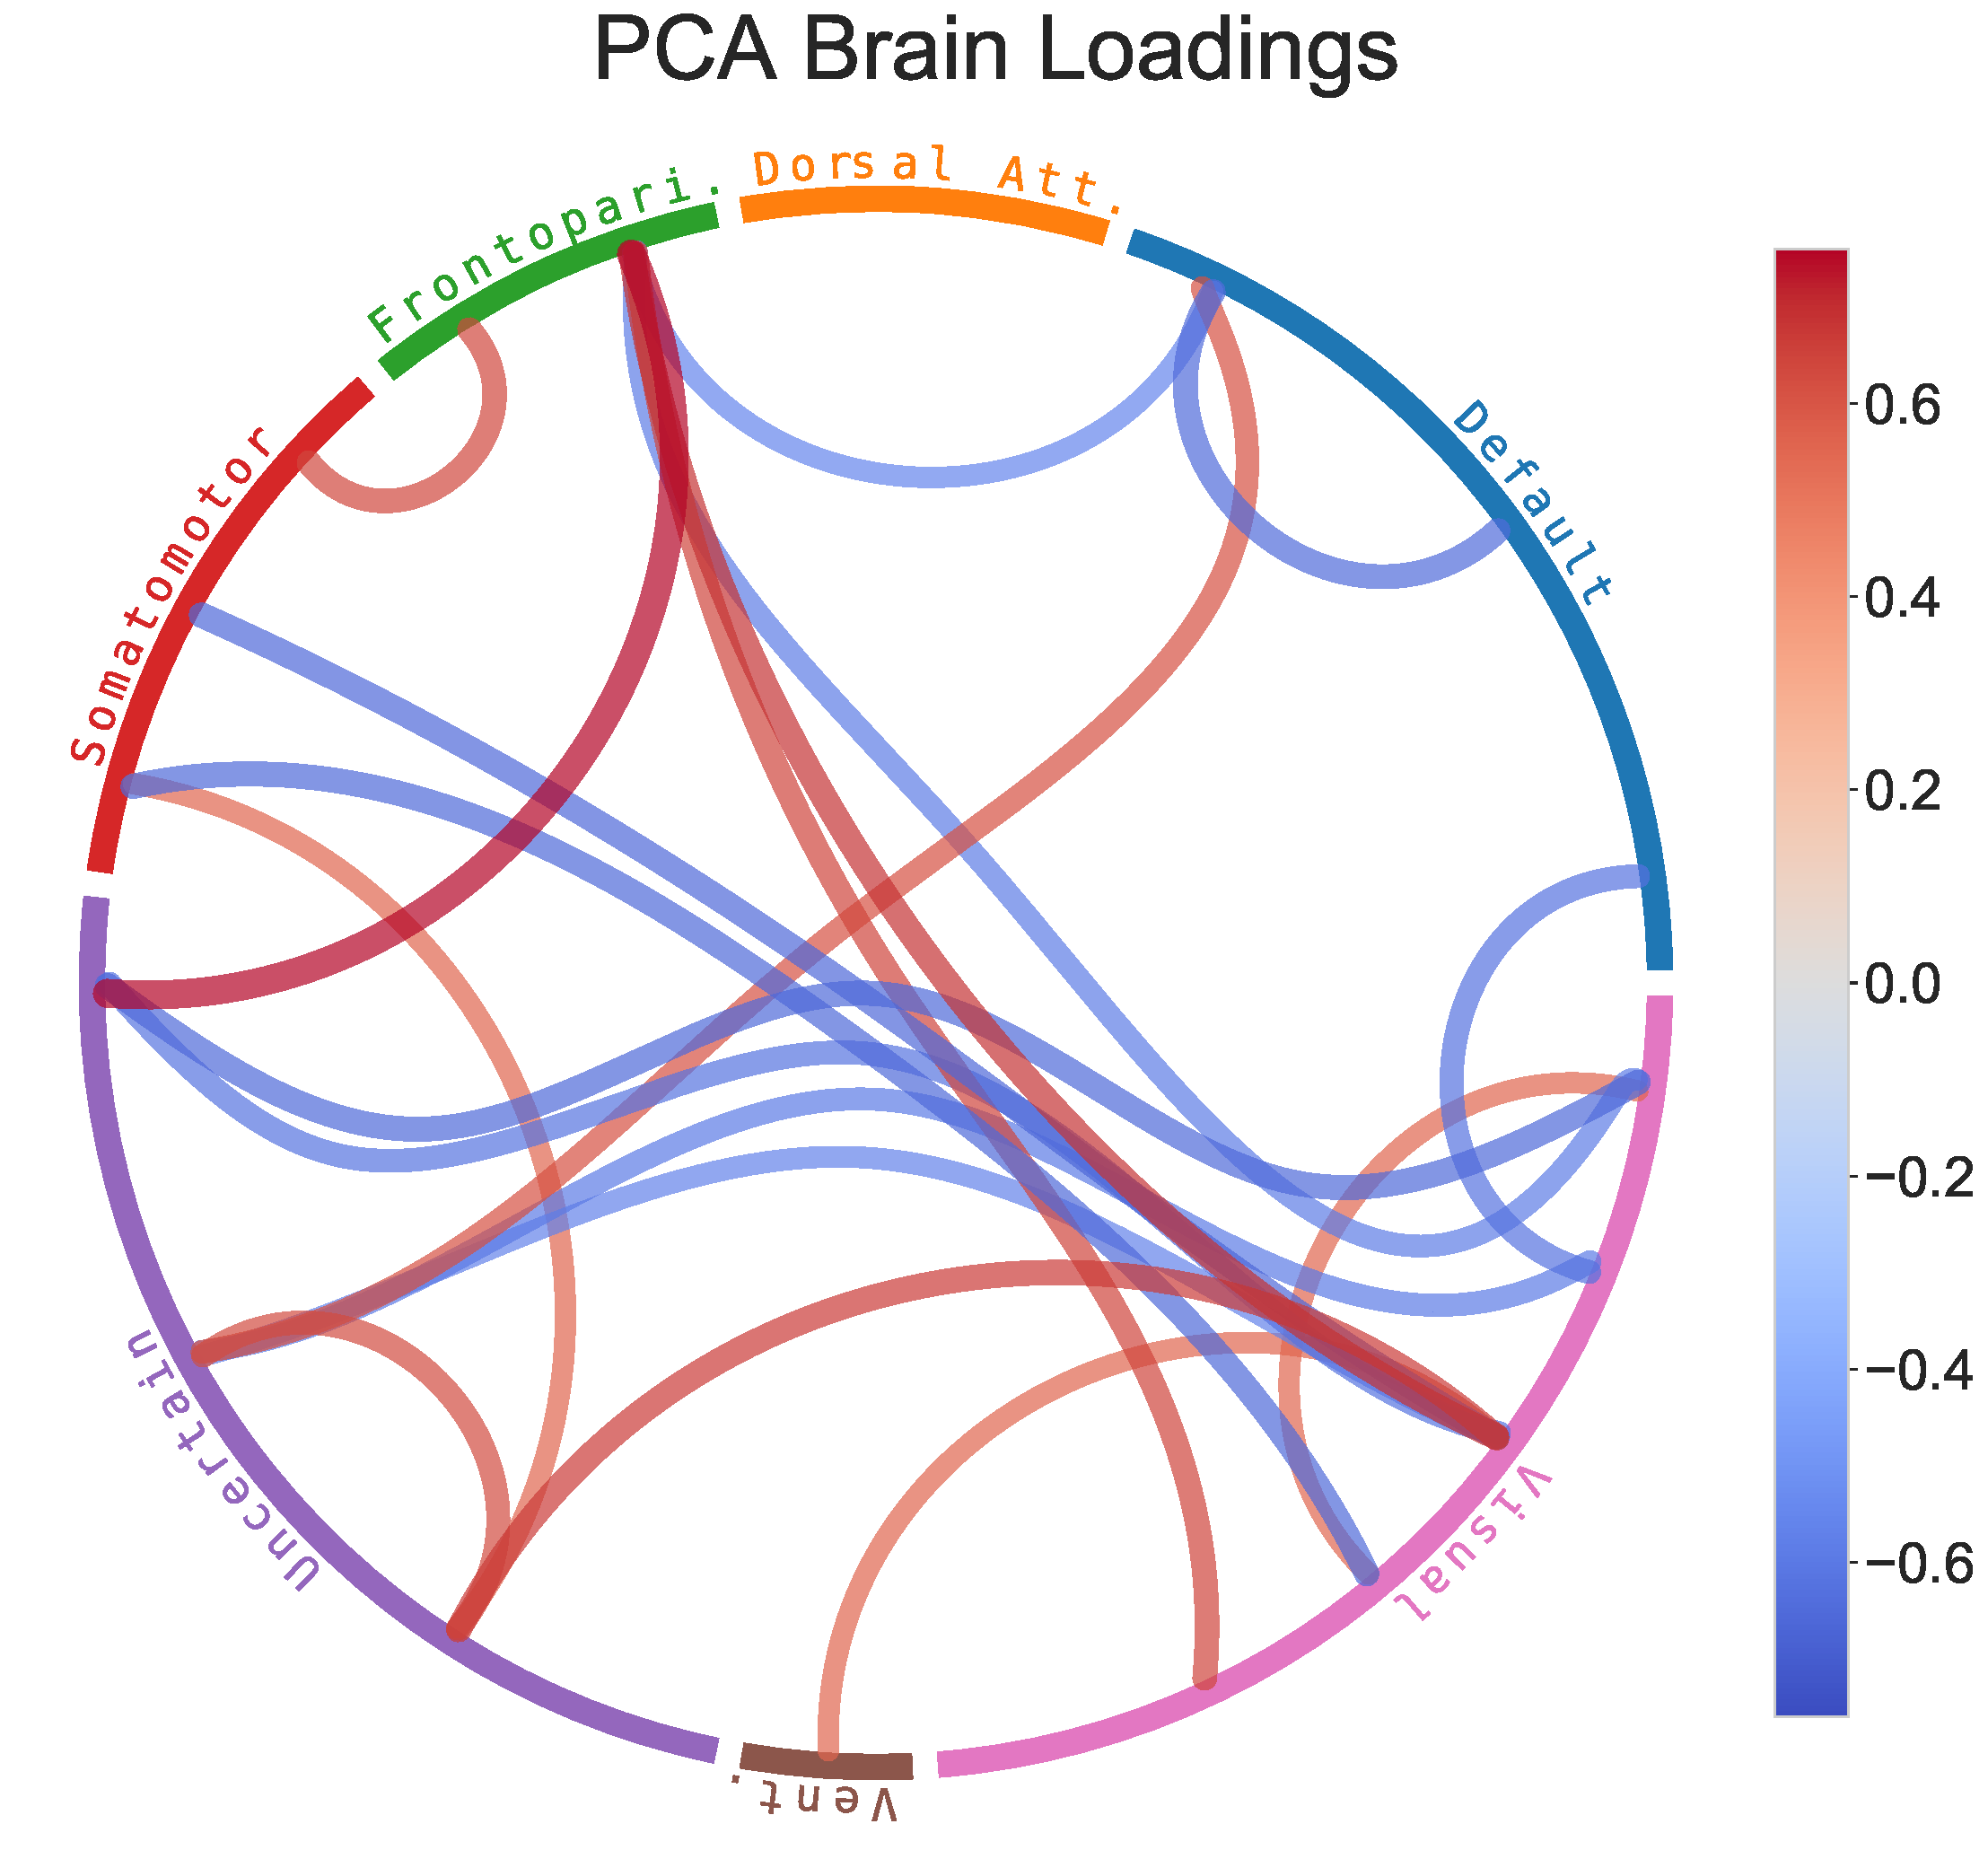
\includegraphics[width=0.49\linewidth]{figures/regularization/hcp/PCA brain loadings.pdf}
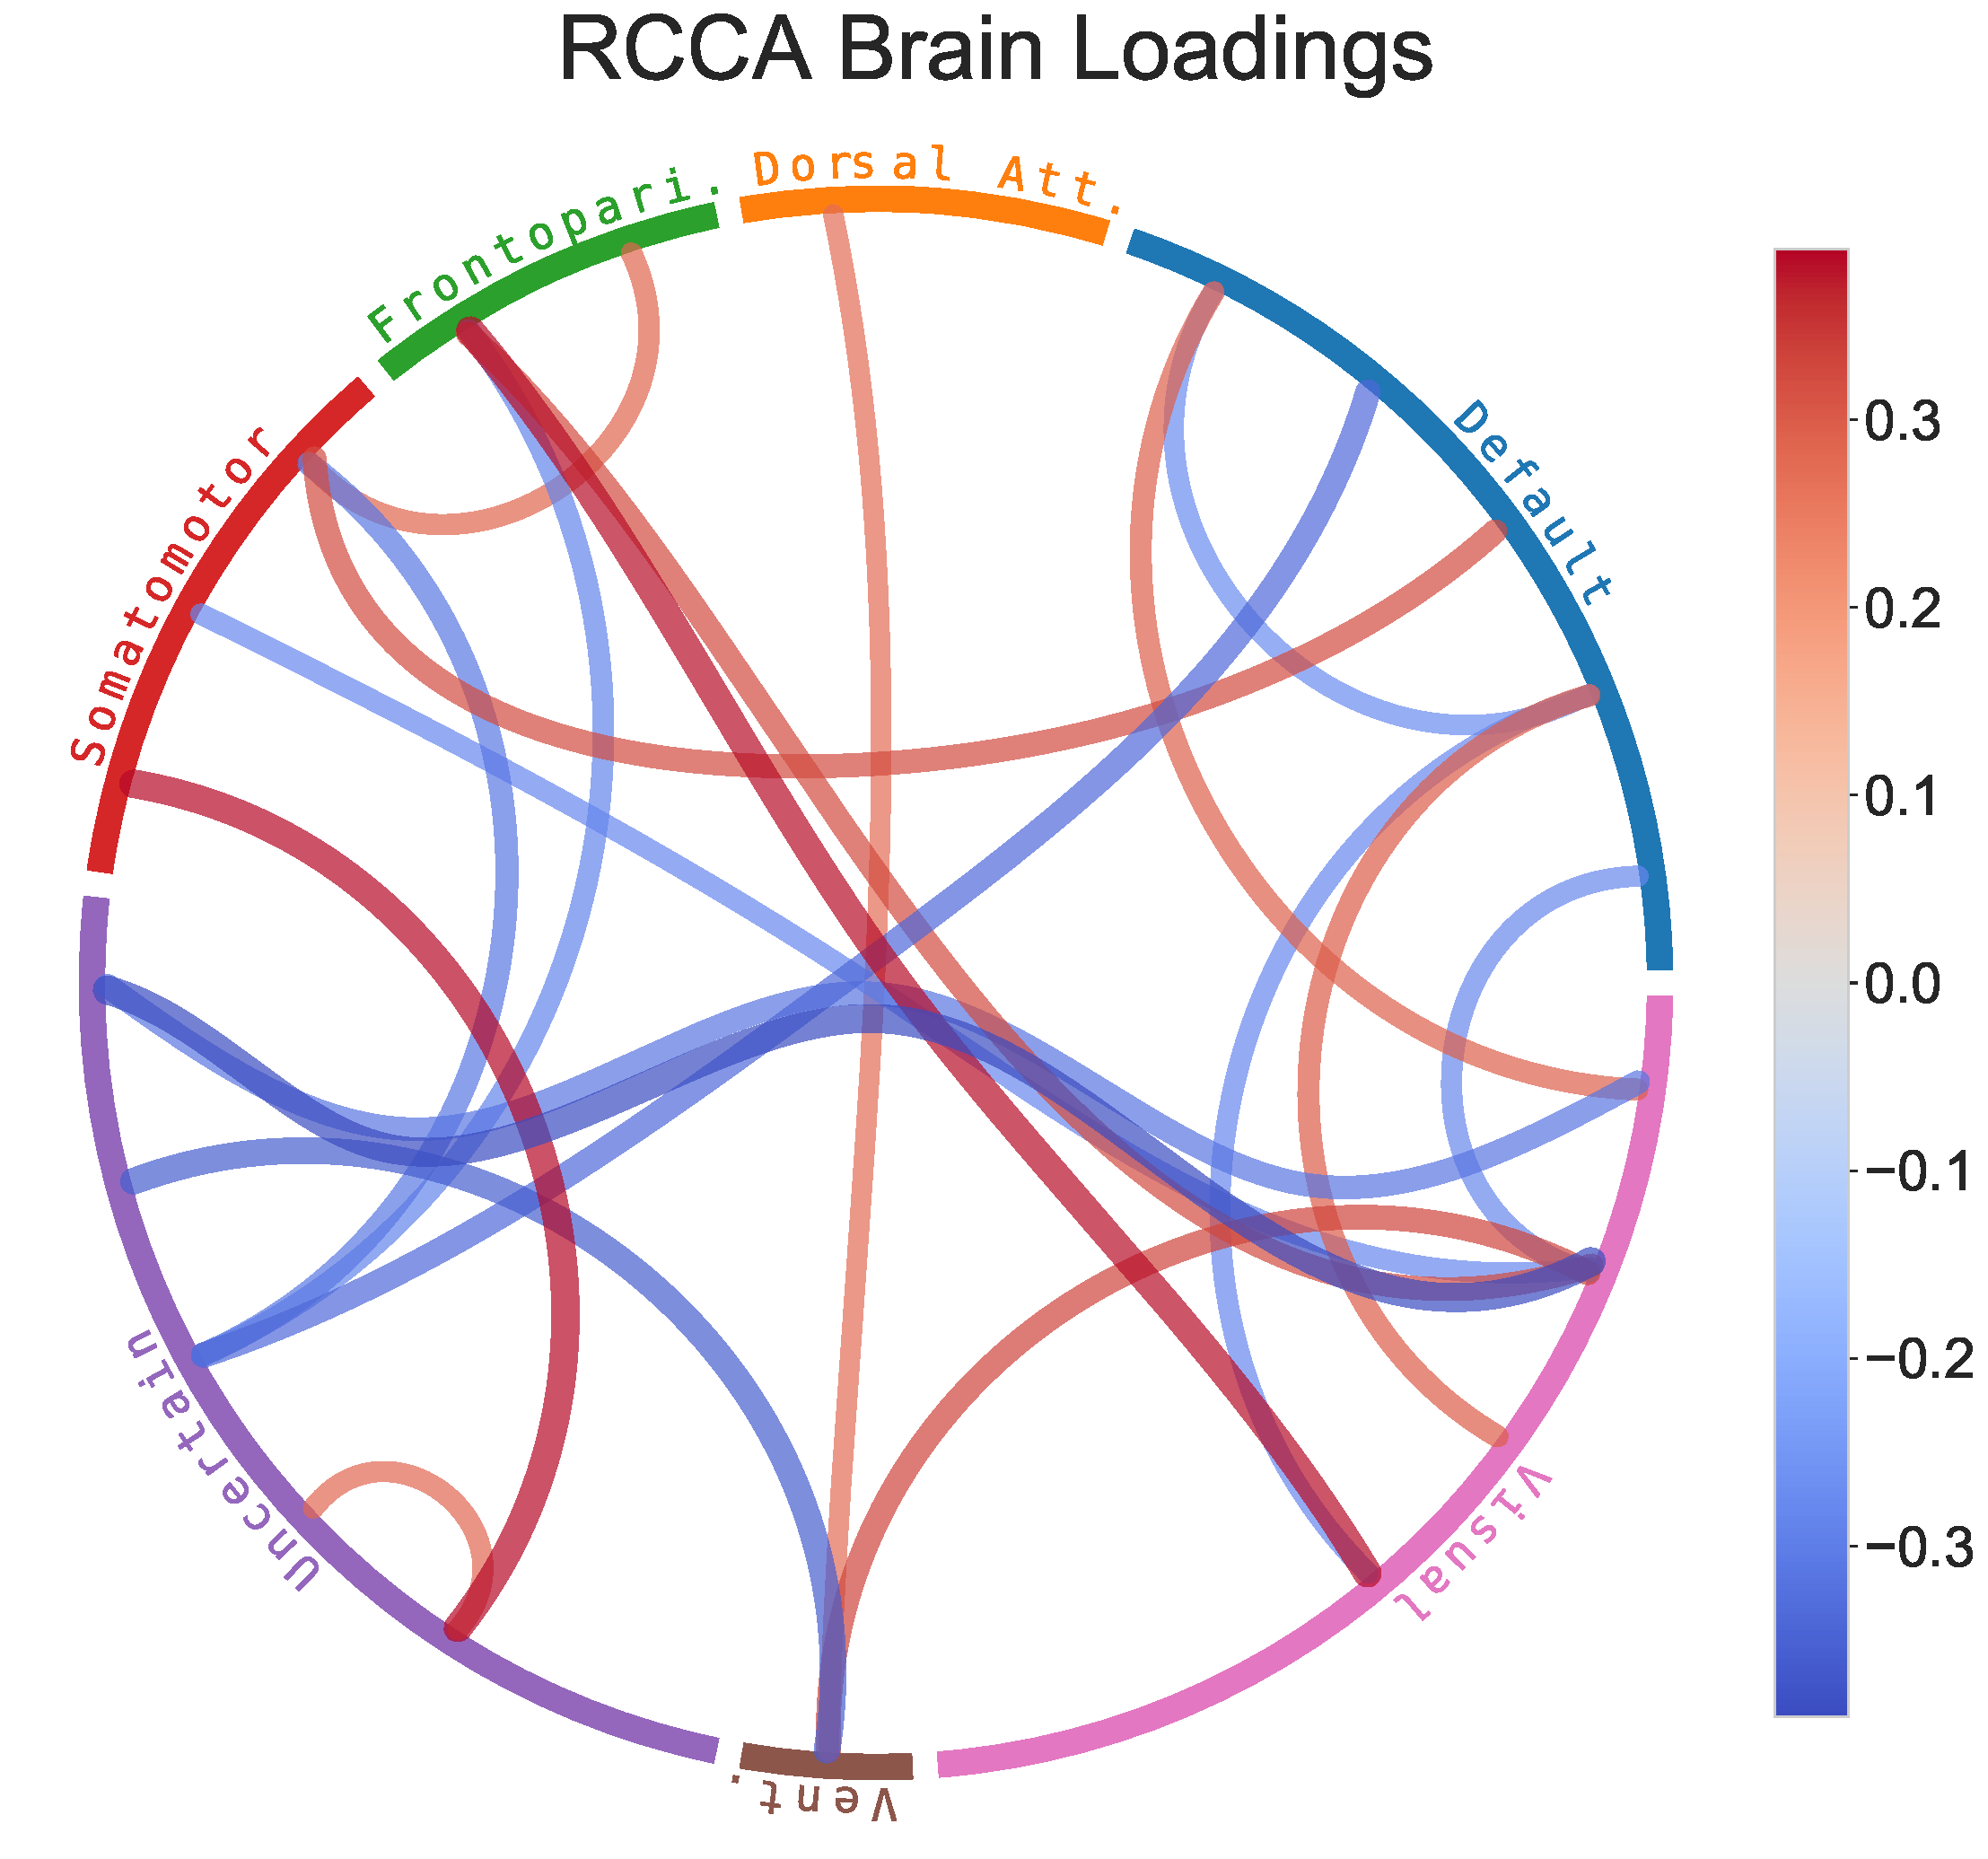
\includegraphics[width=0.49\linewidth]{figures/regularization/hcp/RCCA brain loadings.pdf}
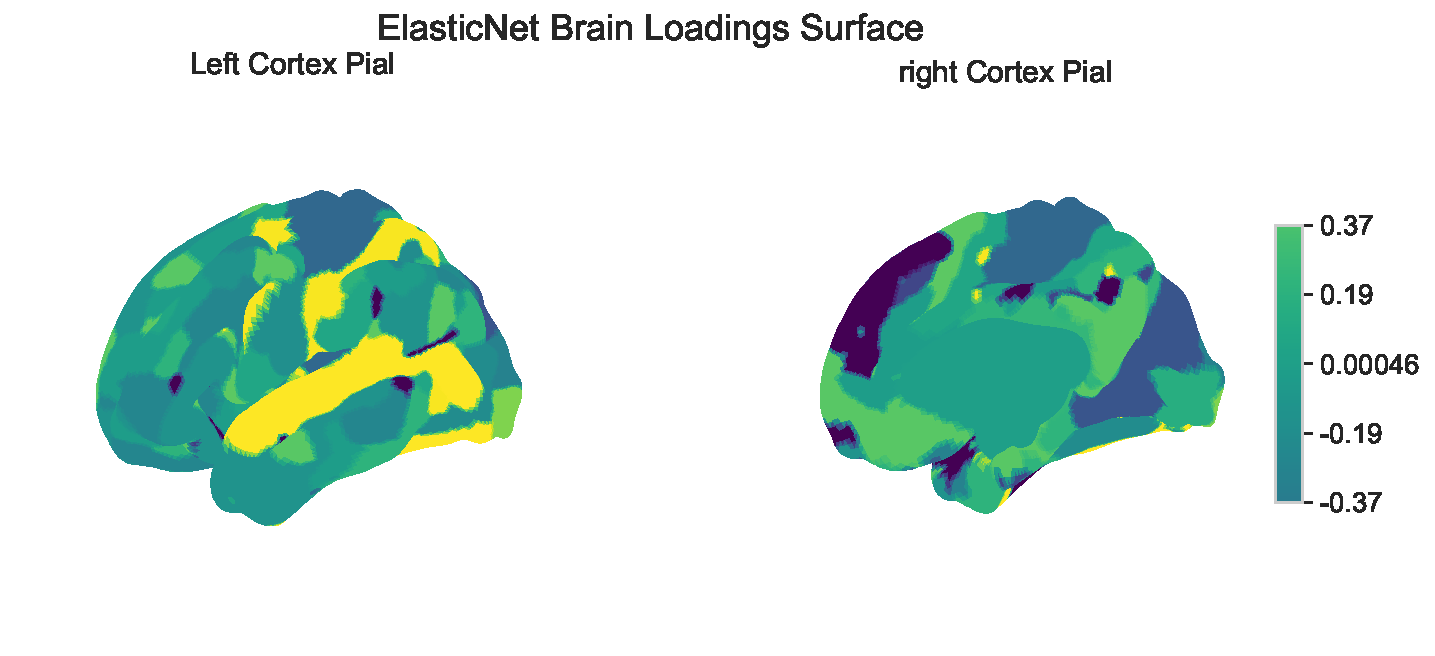
\includegraphics[width=0.49\linewidth]{figures/regularization/hcp/ElasticNet brain loadings.pdf}
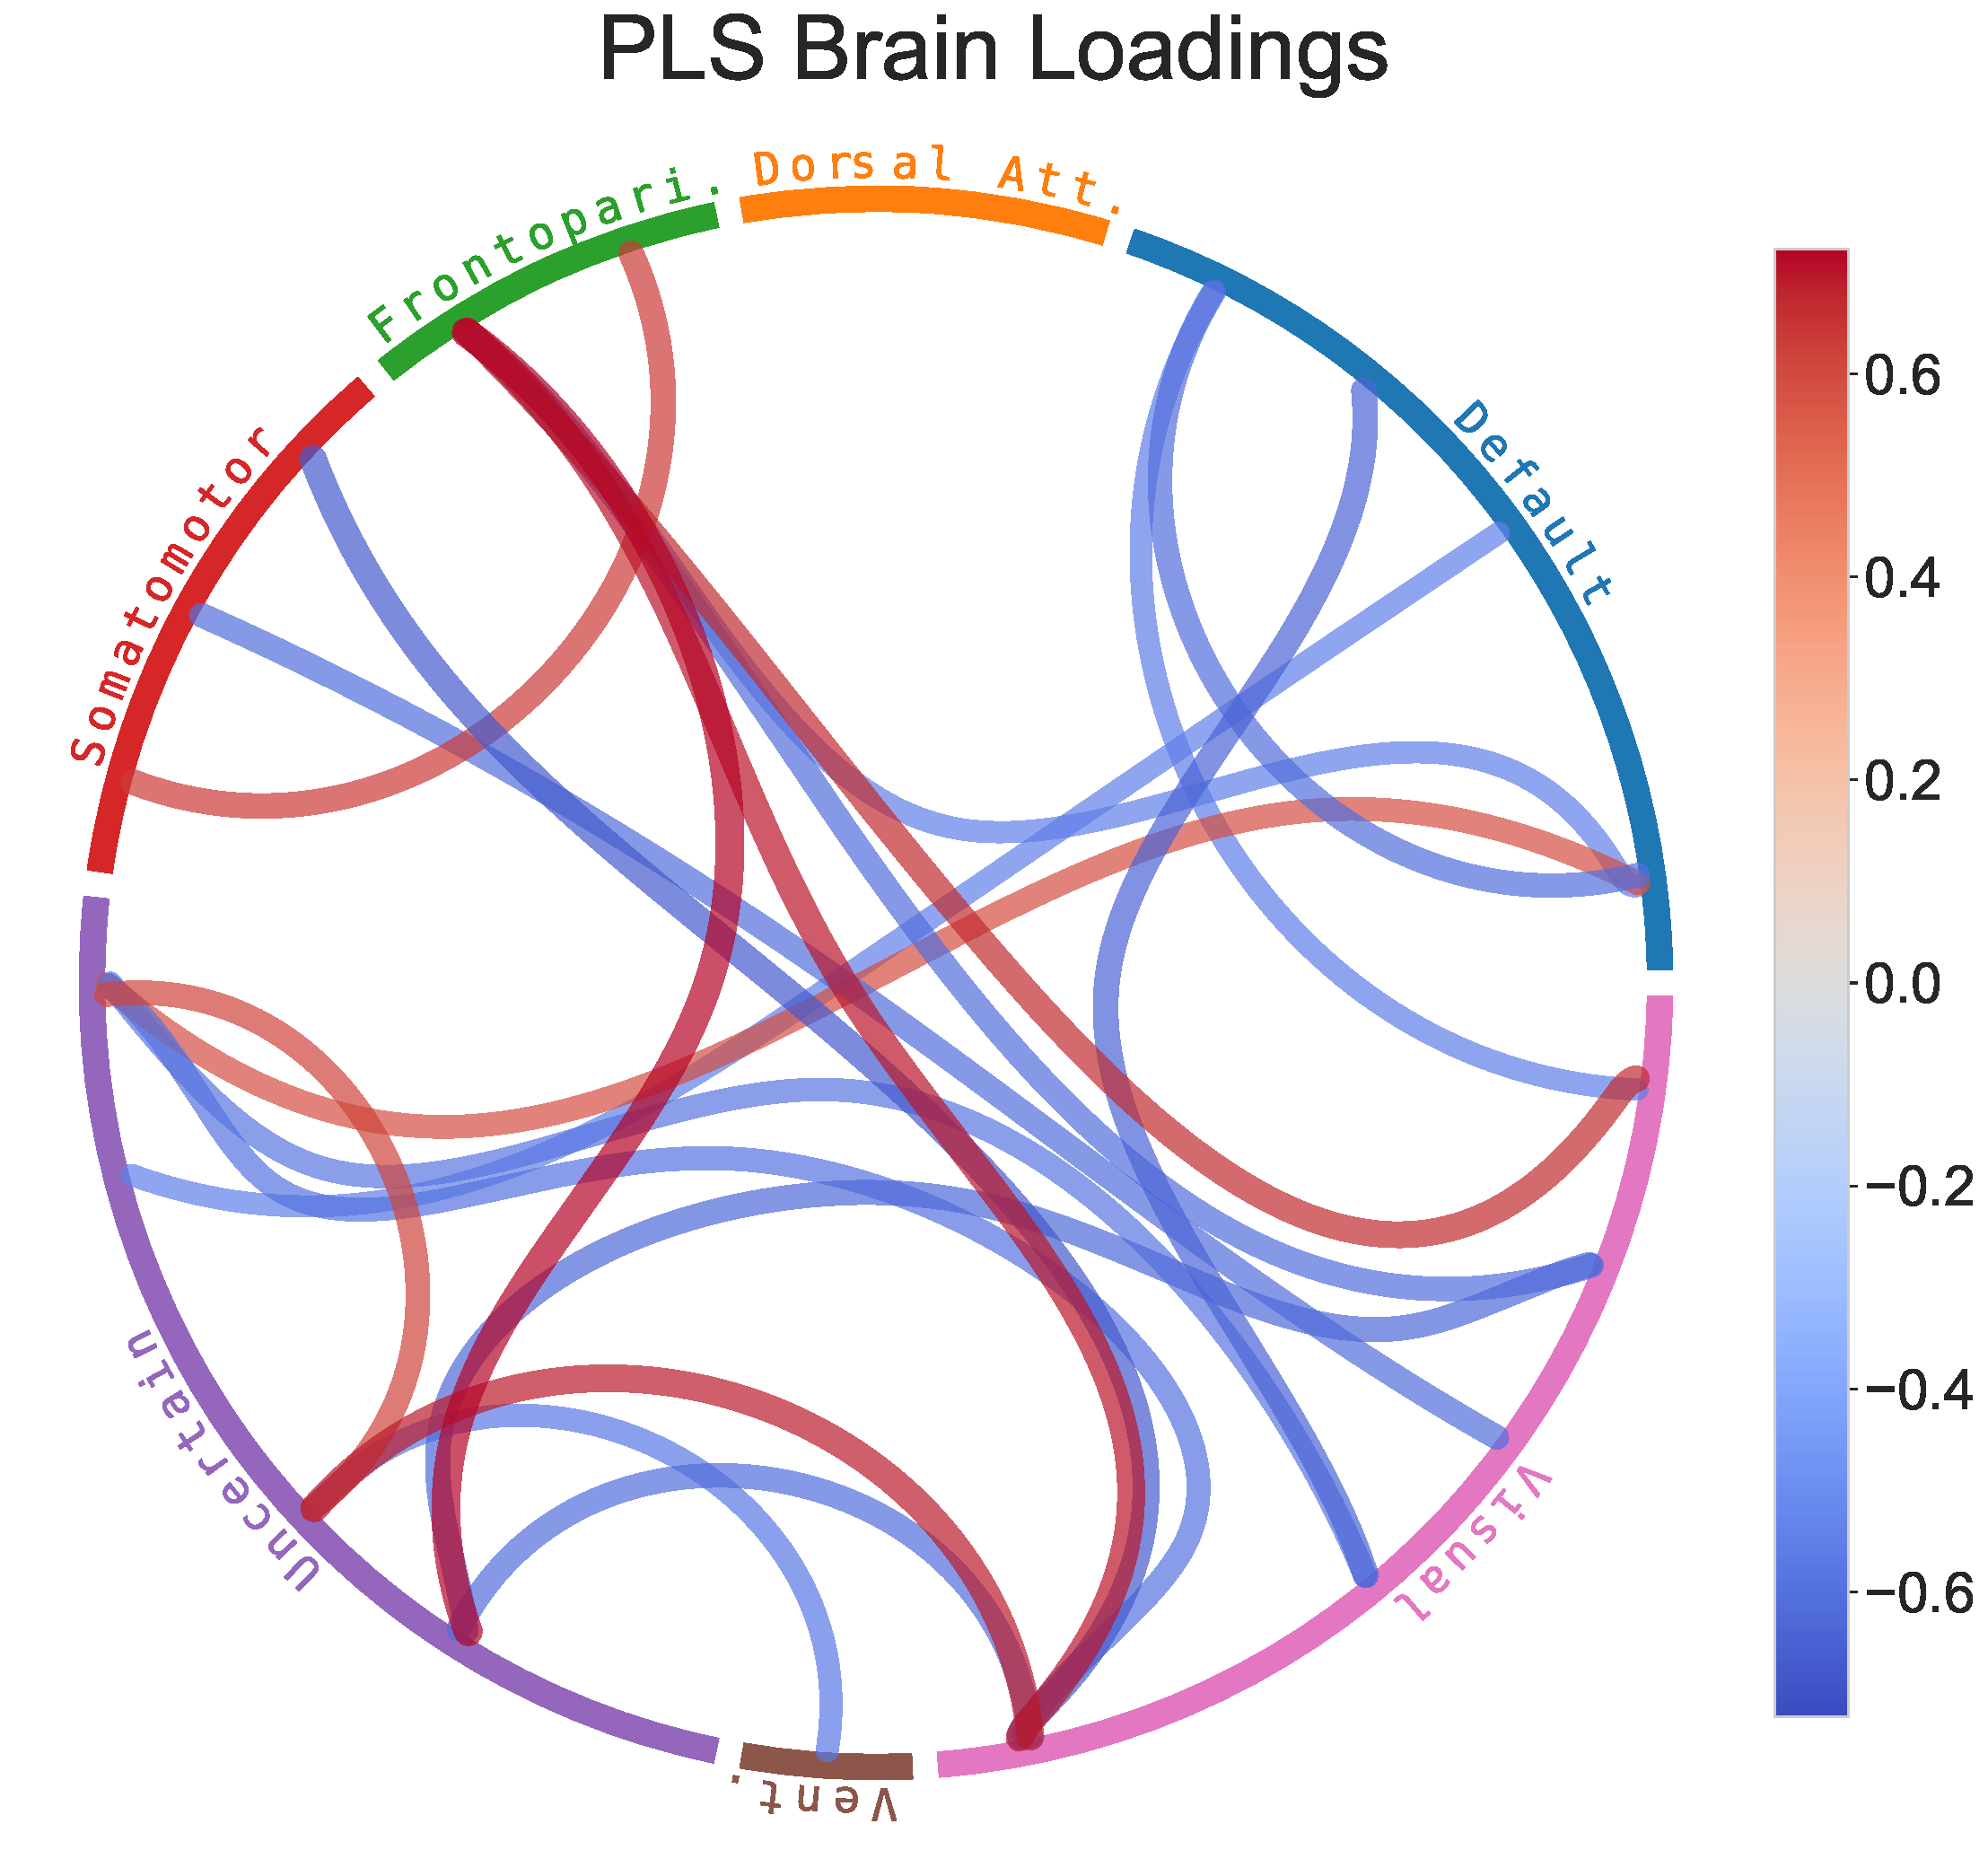
\includegraphics[width=0.49\linewidth]{figures/regularization/hcp/PLS brain loadings.pdf}
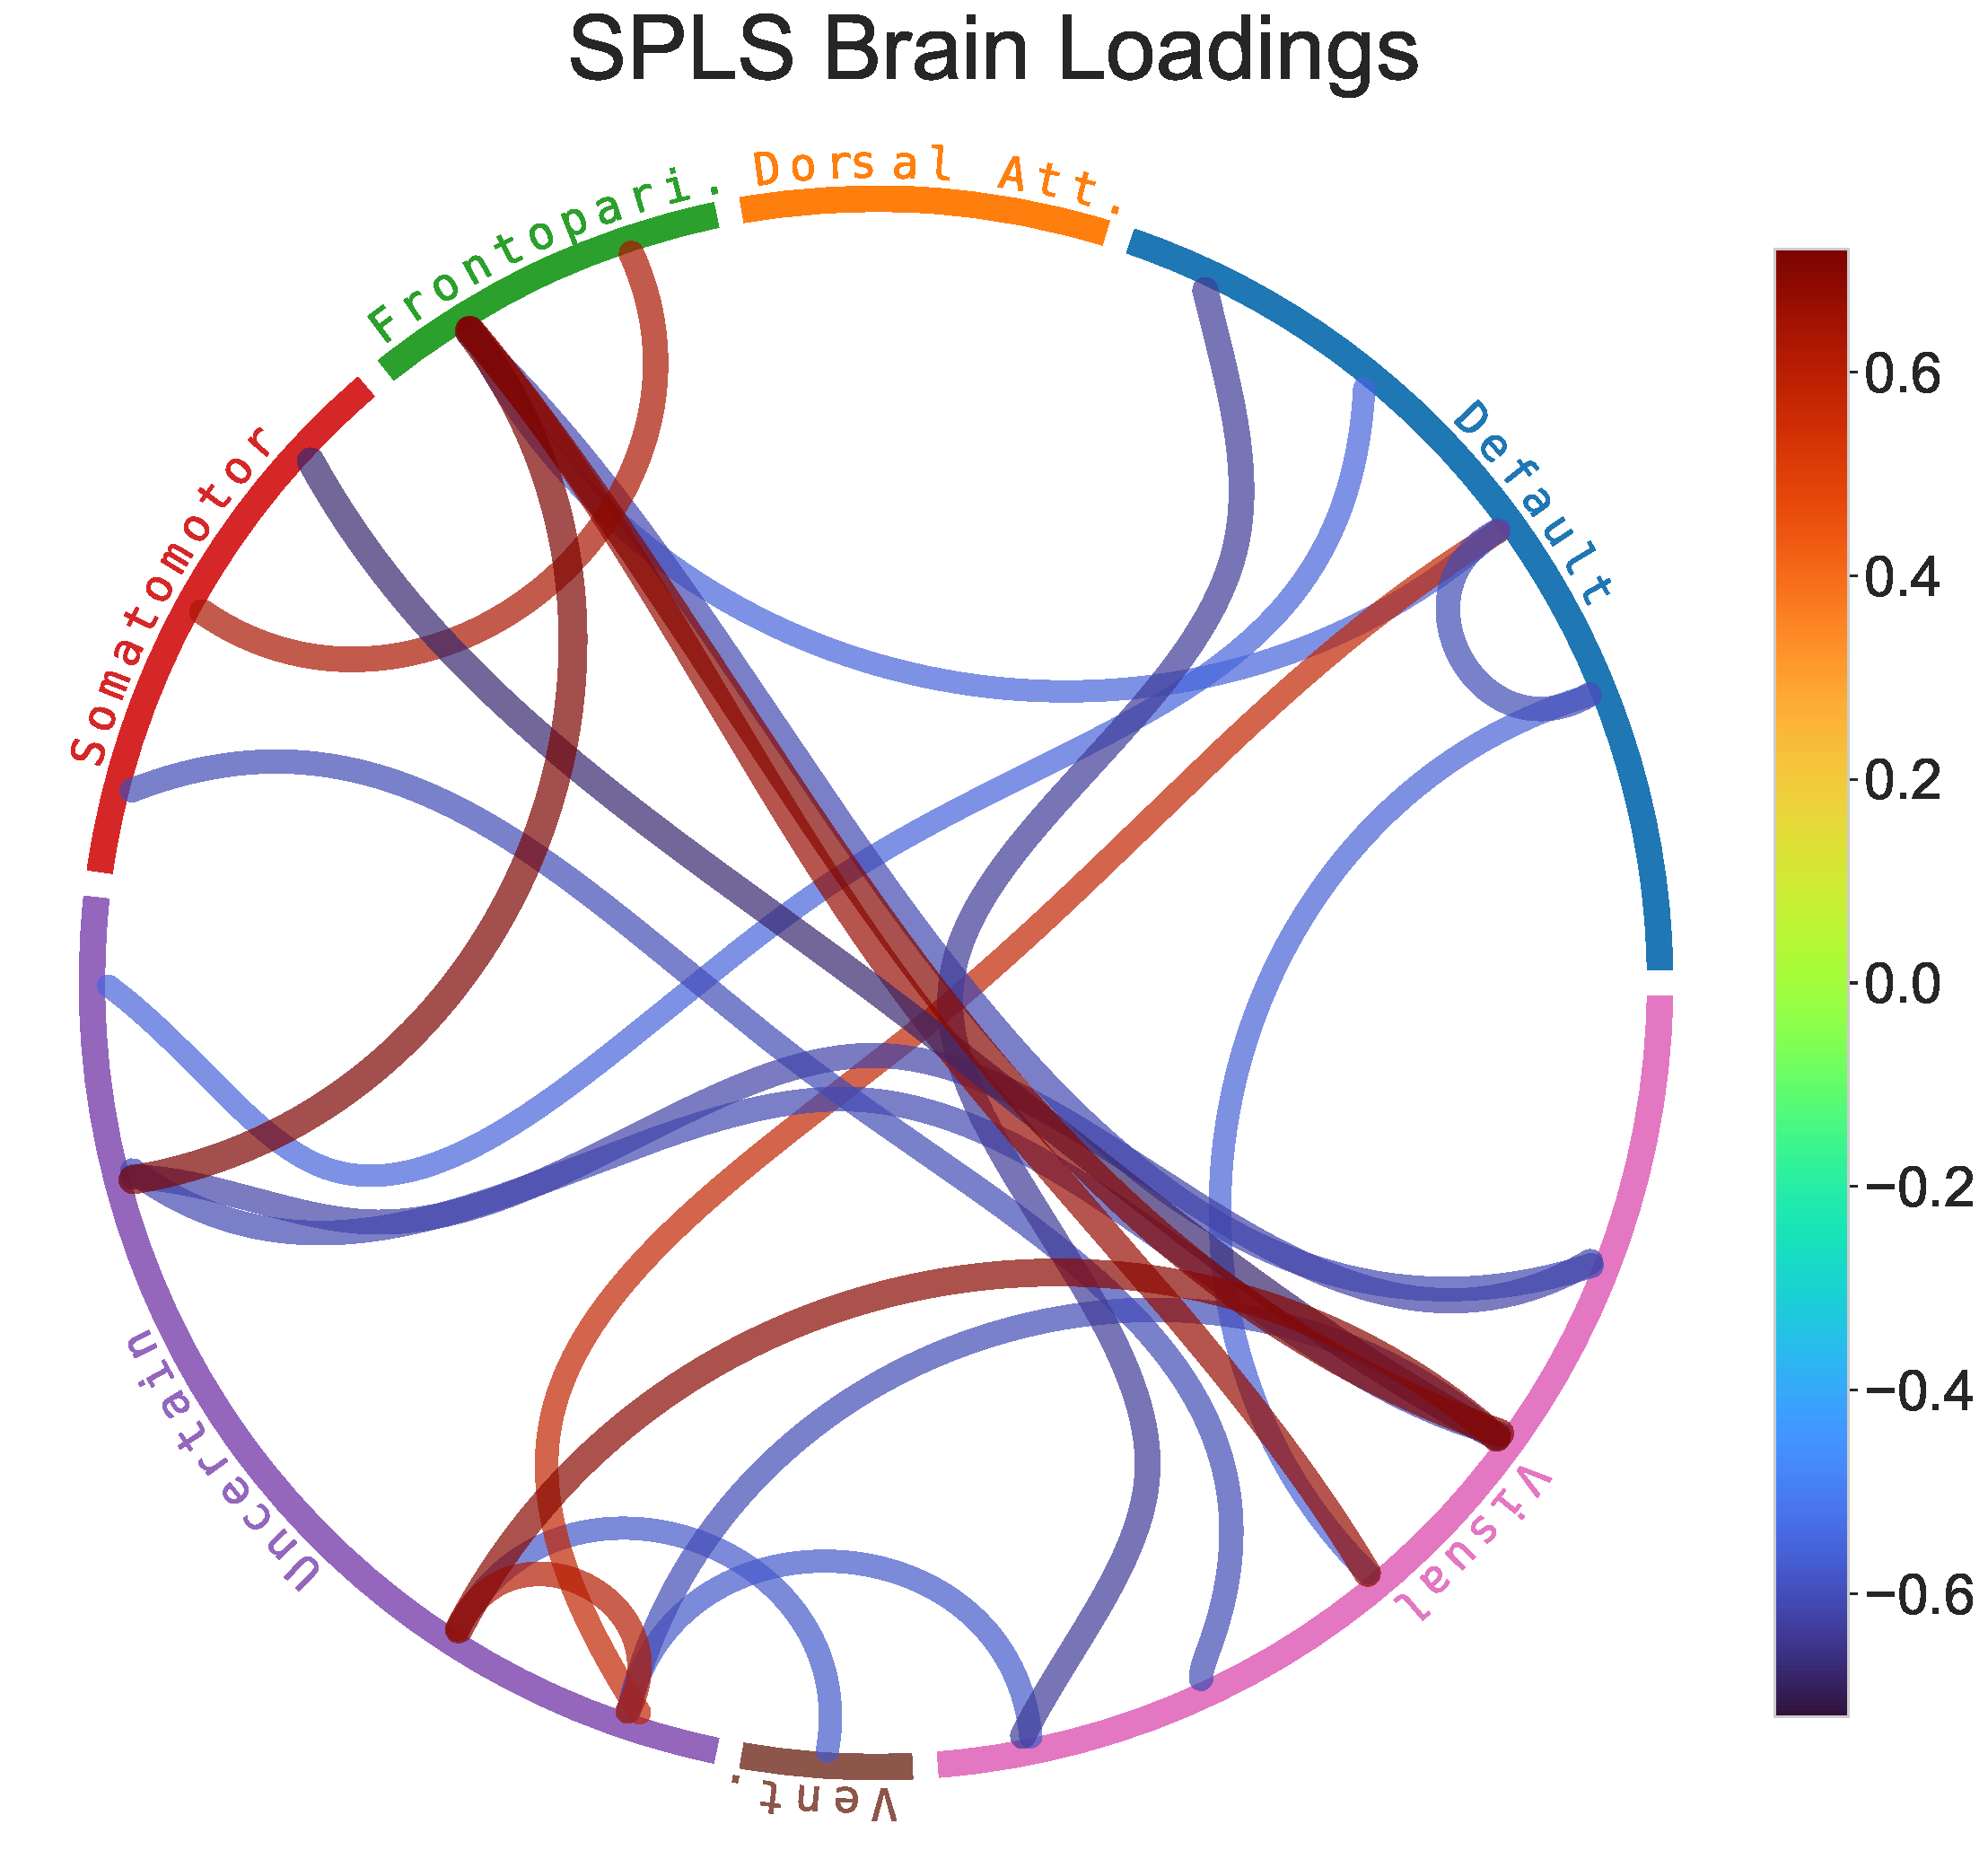
\includegraphics[width=0.49\linewidth]{figures/regularization/hcp/SPLS brain loadings.pdf}
\caption{}\label{}
\end{figure}

\subsubsection{Surface Map Parcellations}
To visualize the brain loadings, we employ a similar approach to \citep{ferreira2022hierarchical, smith2015positive}.
The brain surface plots in Figure~\ref{fig:brain} thus represent maps of brain connection strength increases/decreases, which
were obtained by weighting each node’s parcel map with the GFA edge-strengths summed across the edges
connected to the node.

\begin{figure}
\centering
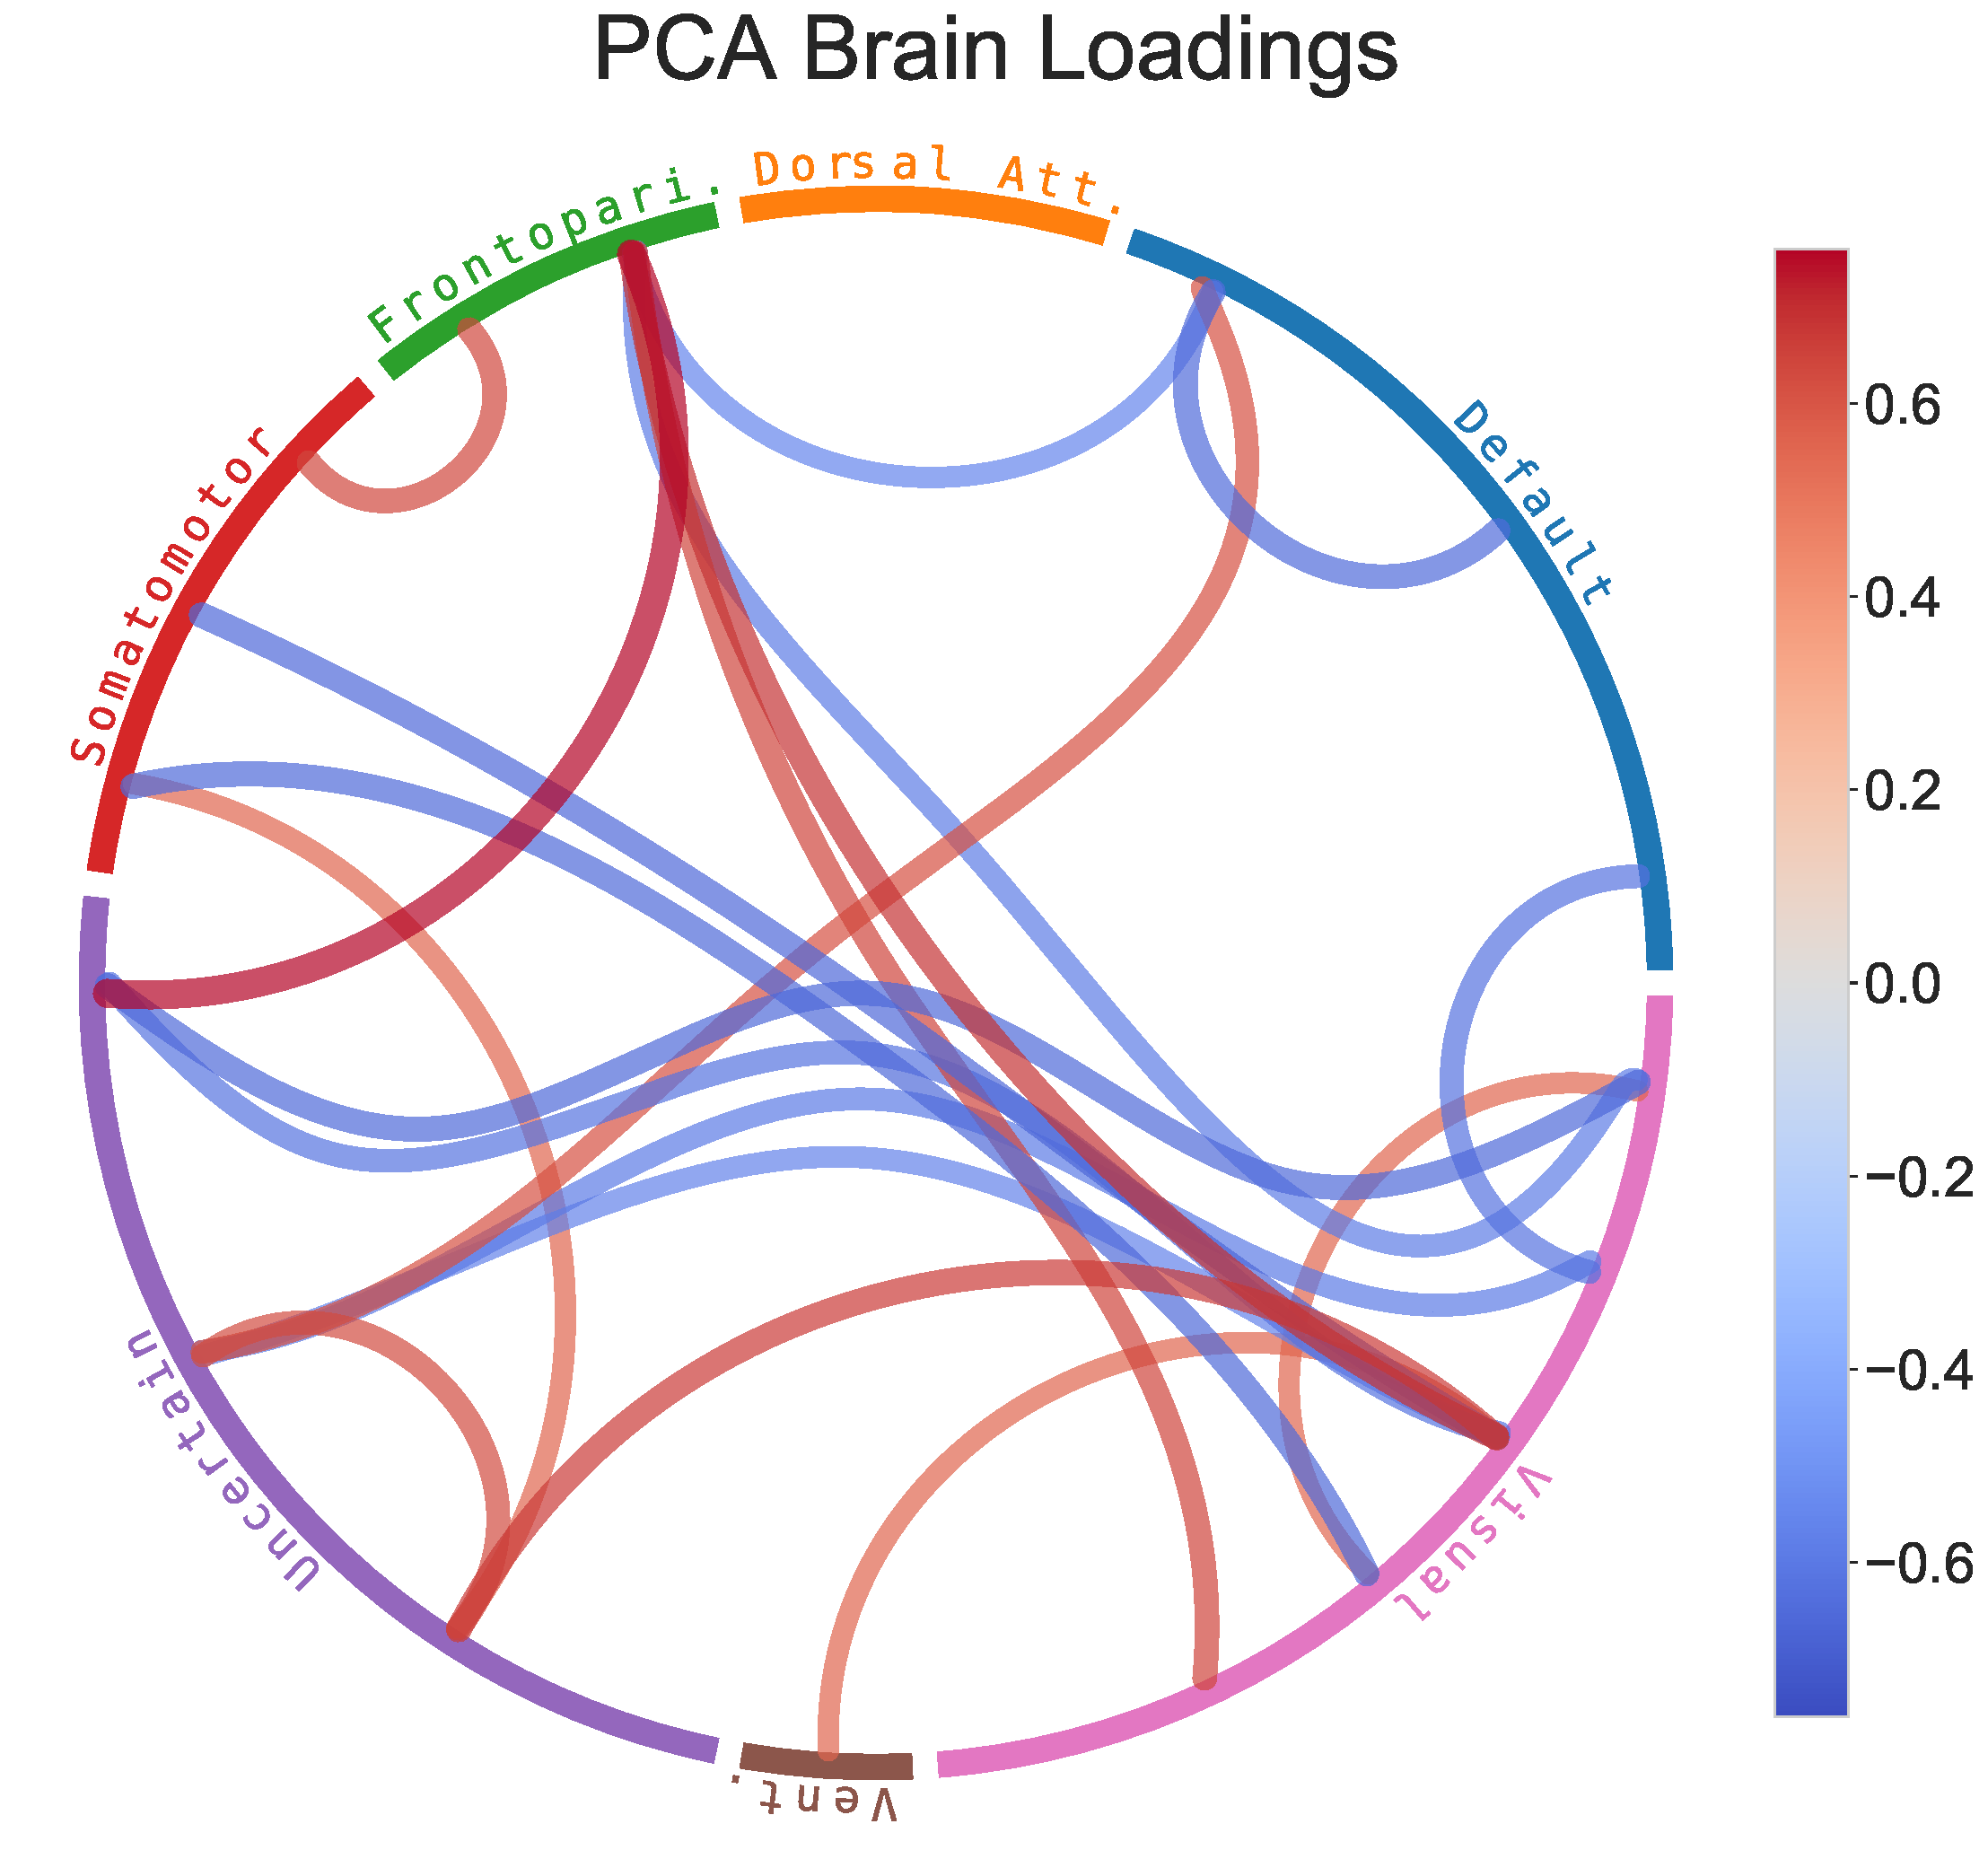
\includegraphics[width=0.68\linewidth]{figures/regularization/hcp/PCA brain loadings.pdf}
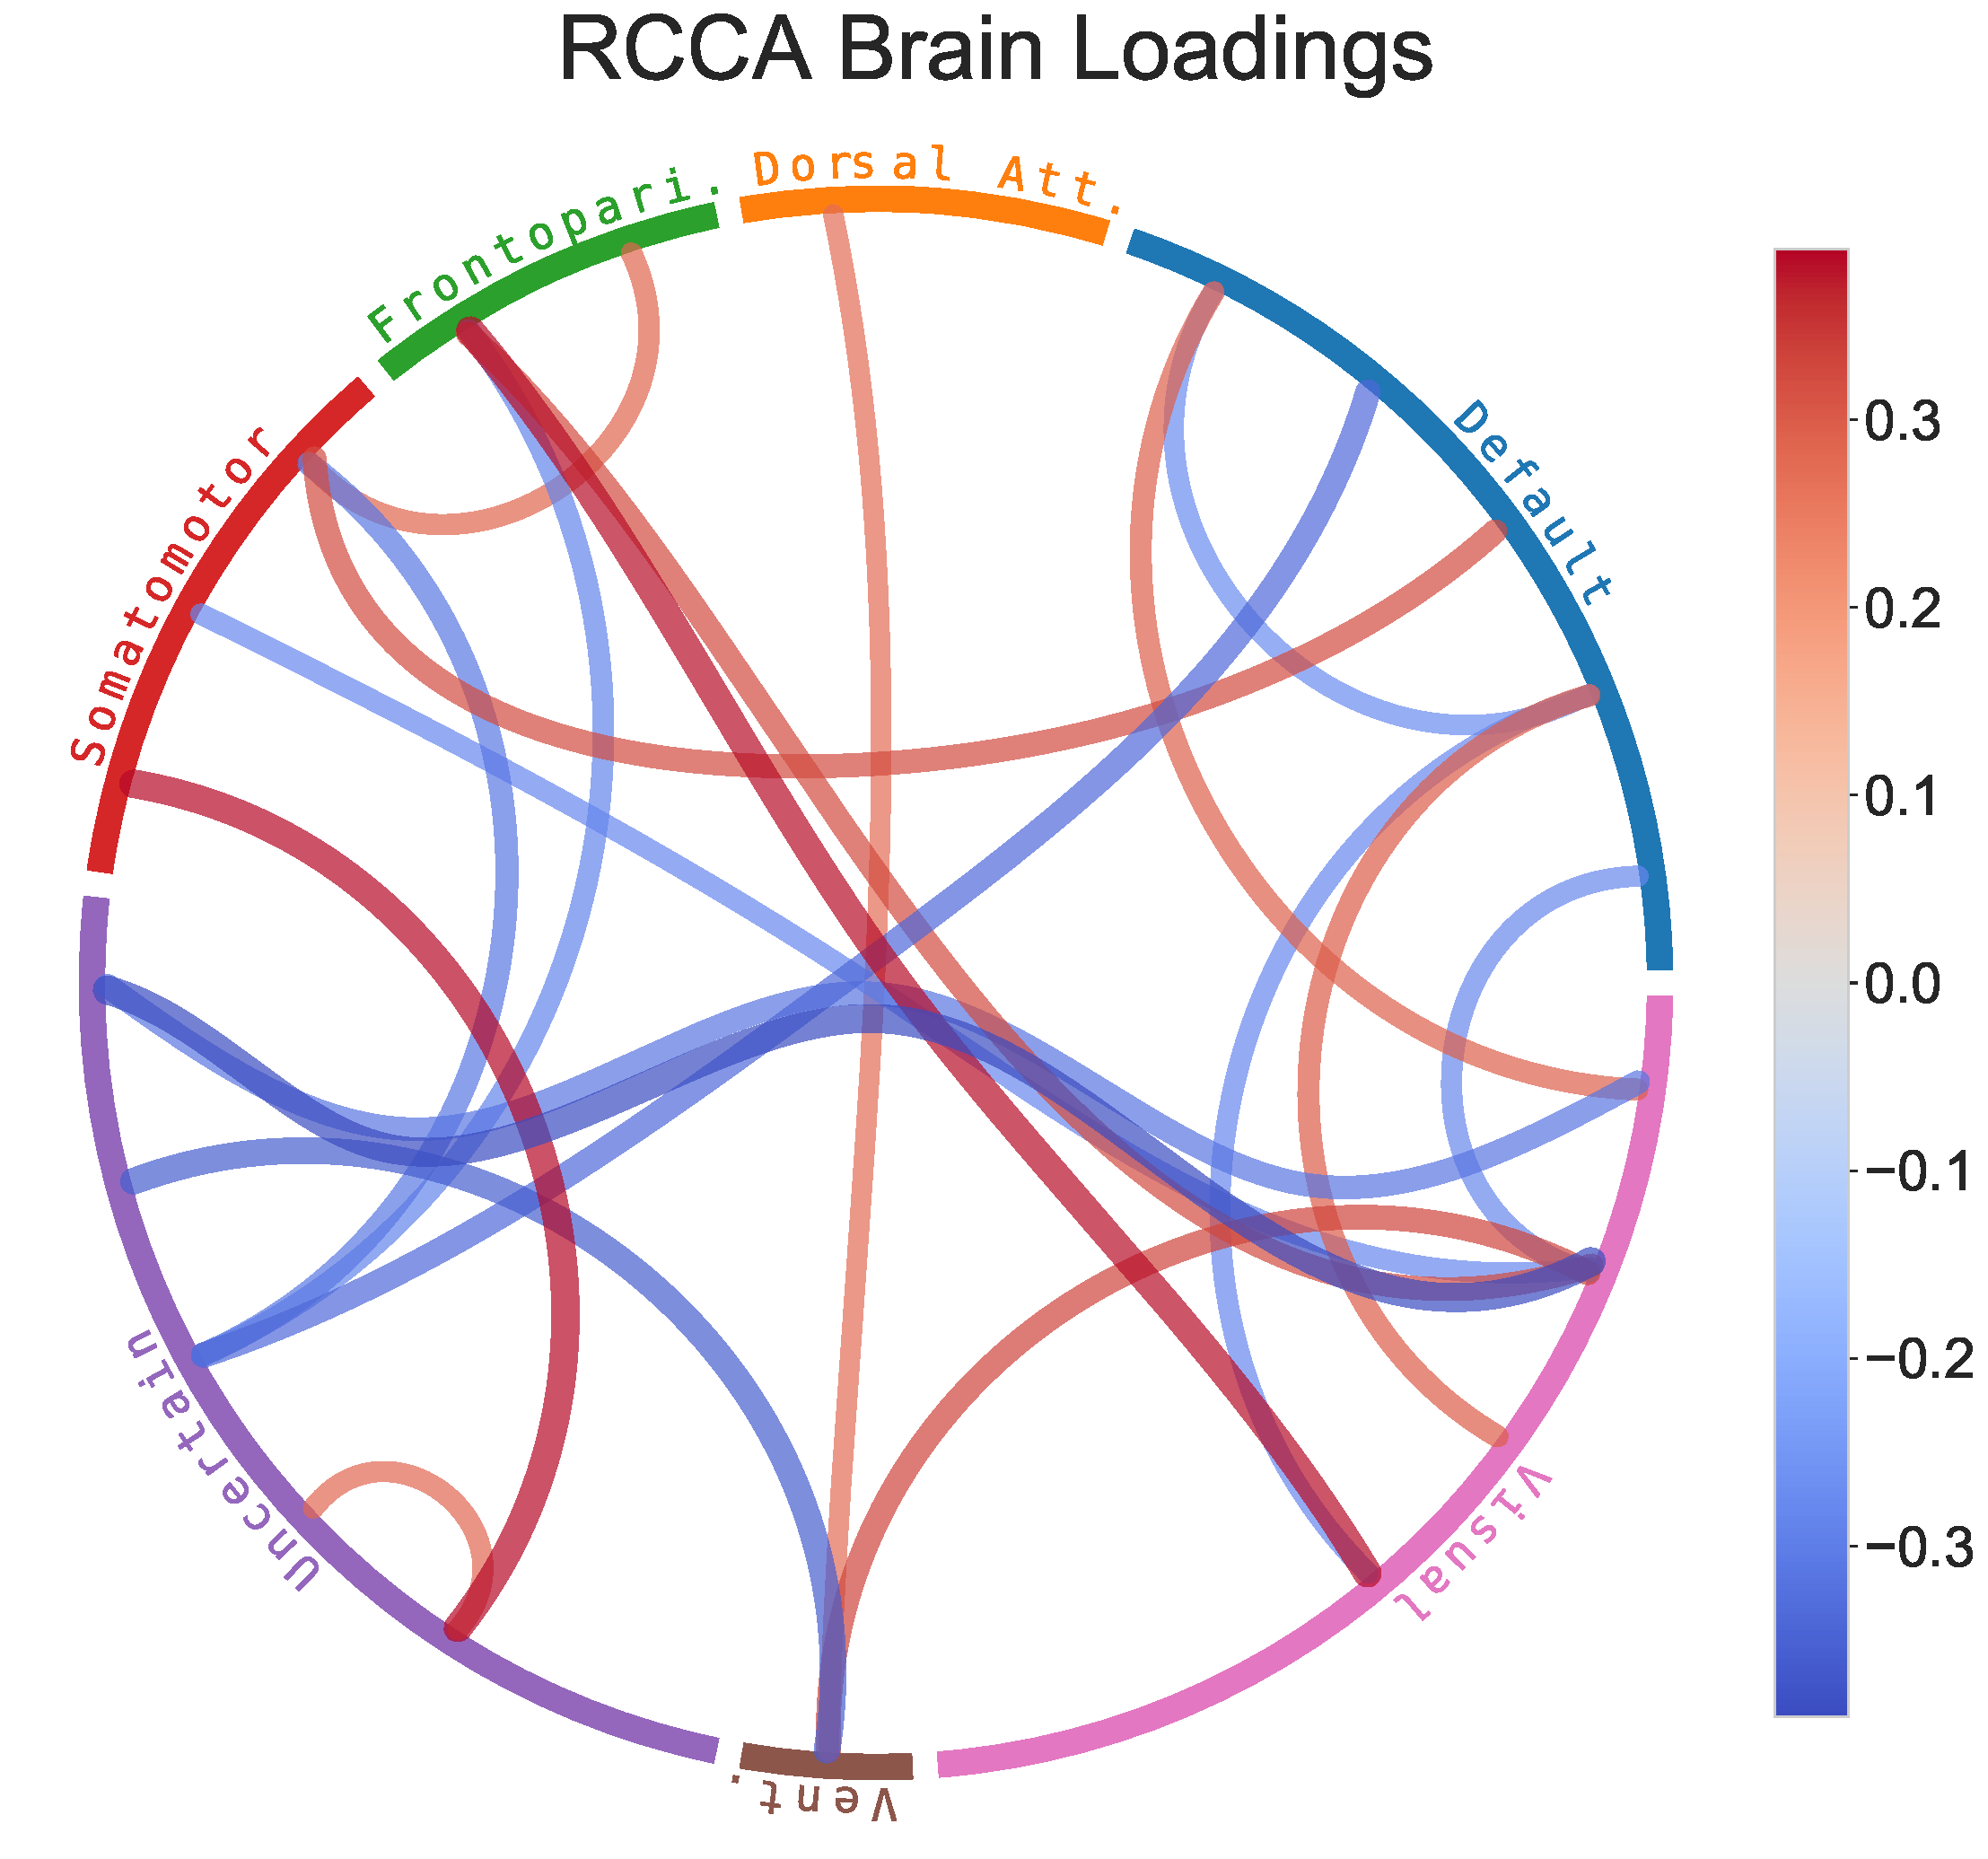
\includegraphics[width=0.68\linewidth]{figures/regularization/hcp/RCCA brain loadings.pdf}
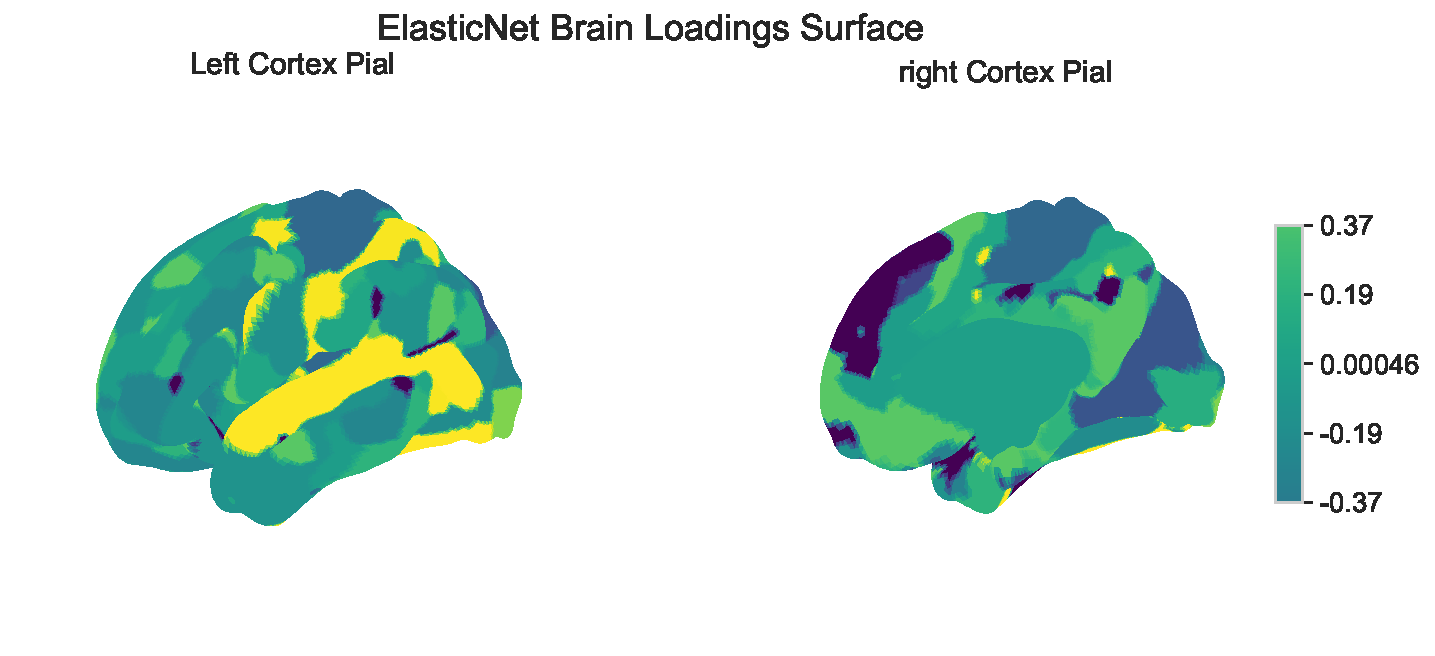
\includegraphics[width=0.68\linewidth]{figures/regularization/hcp/ElasticNet brain loadings.pdf}
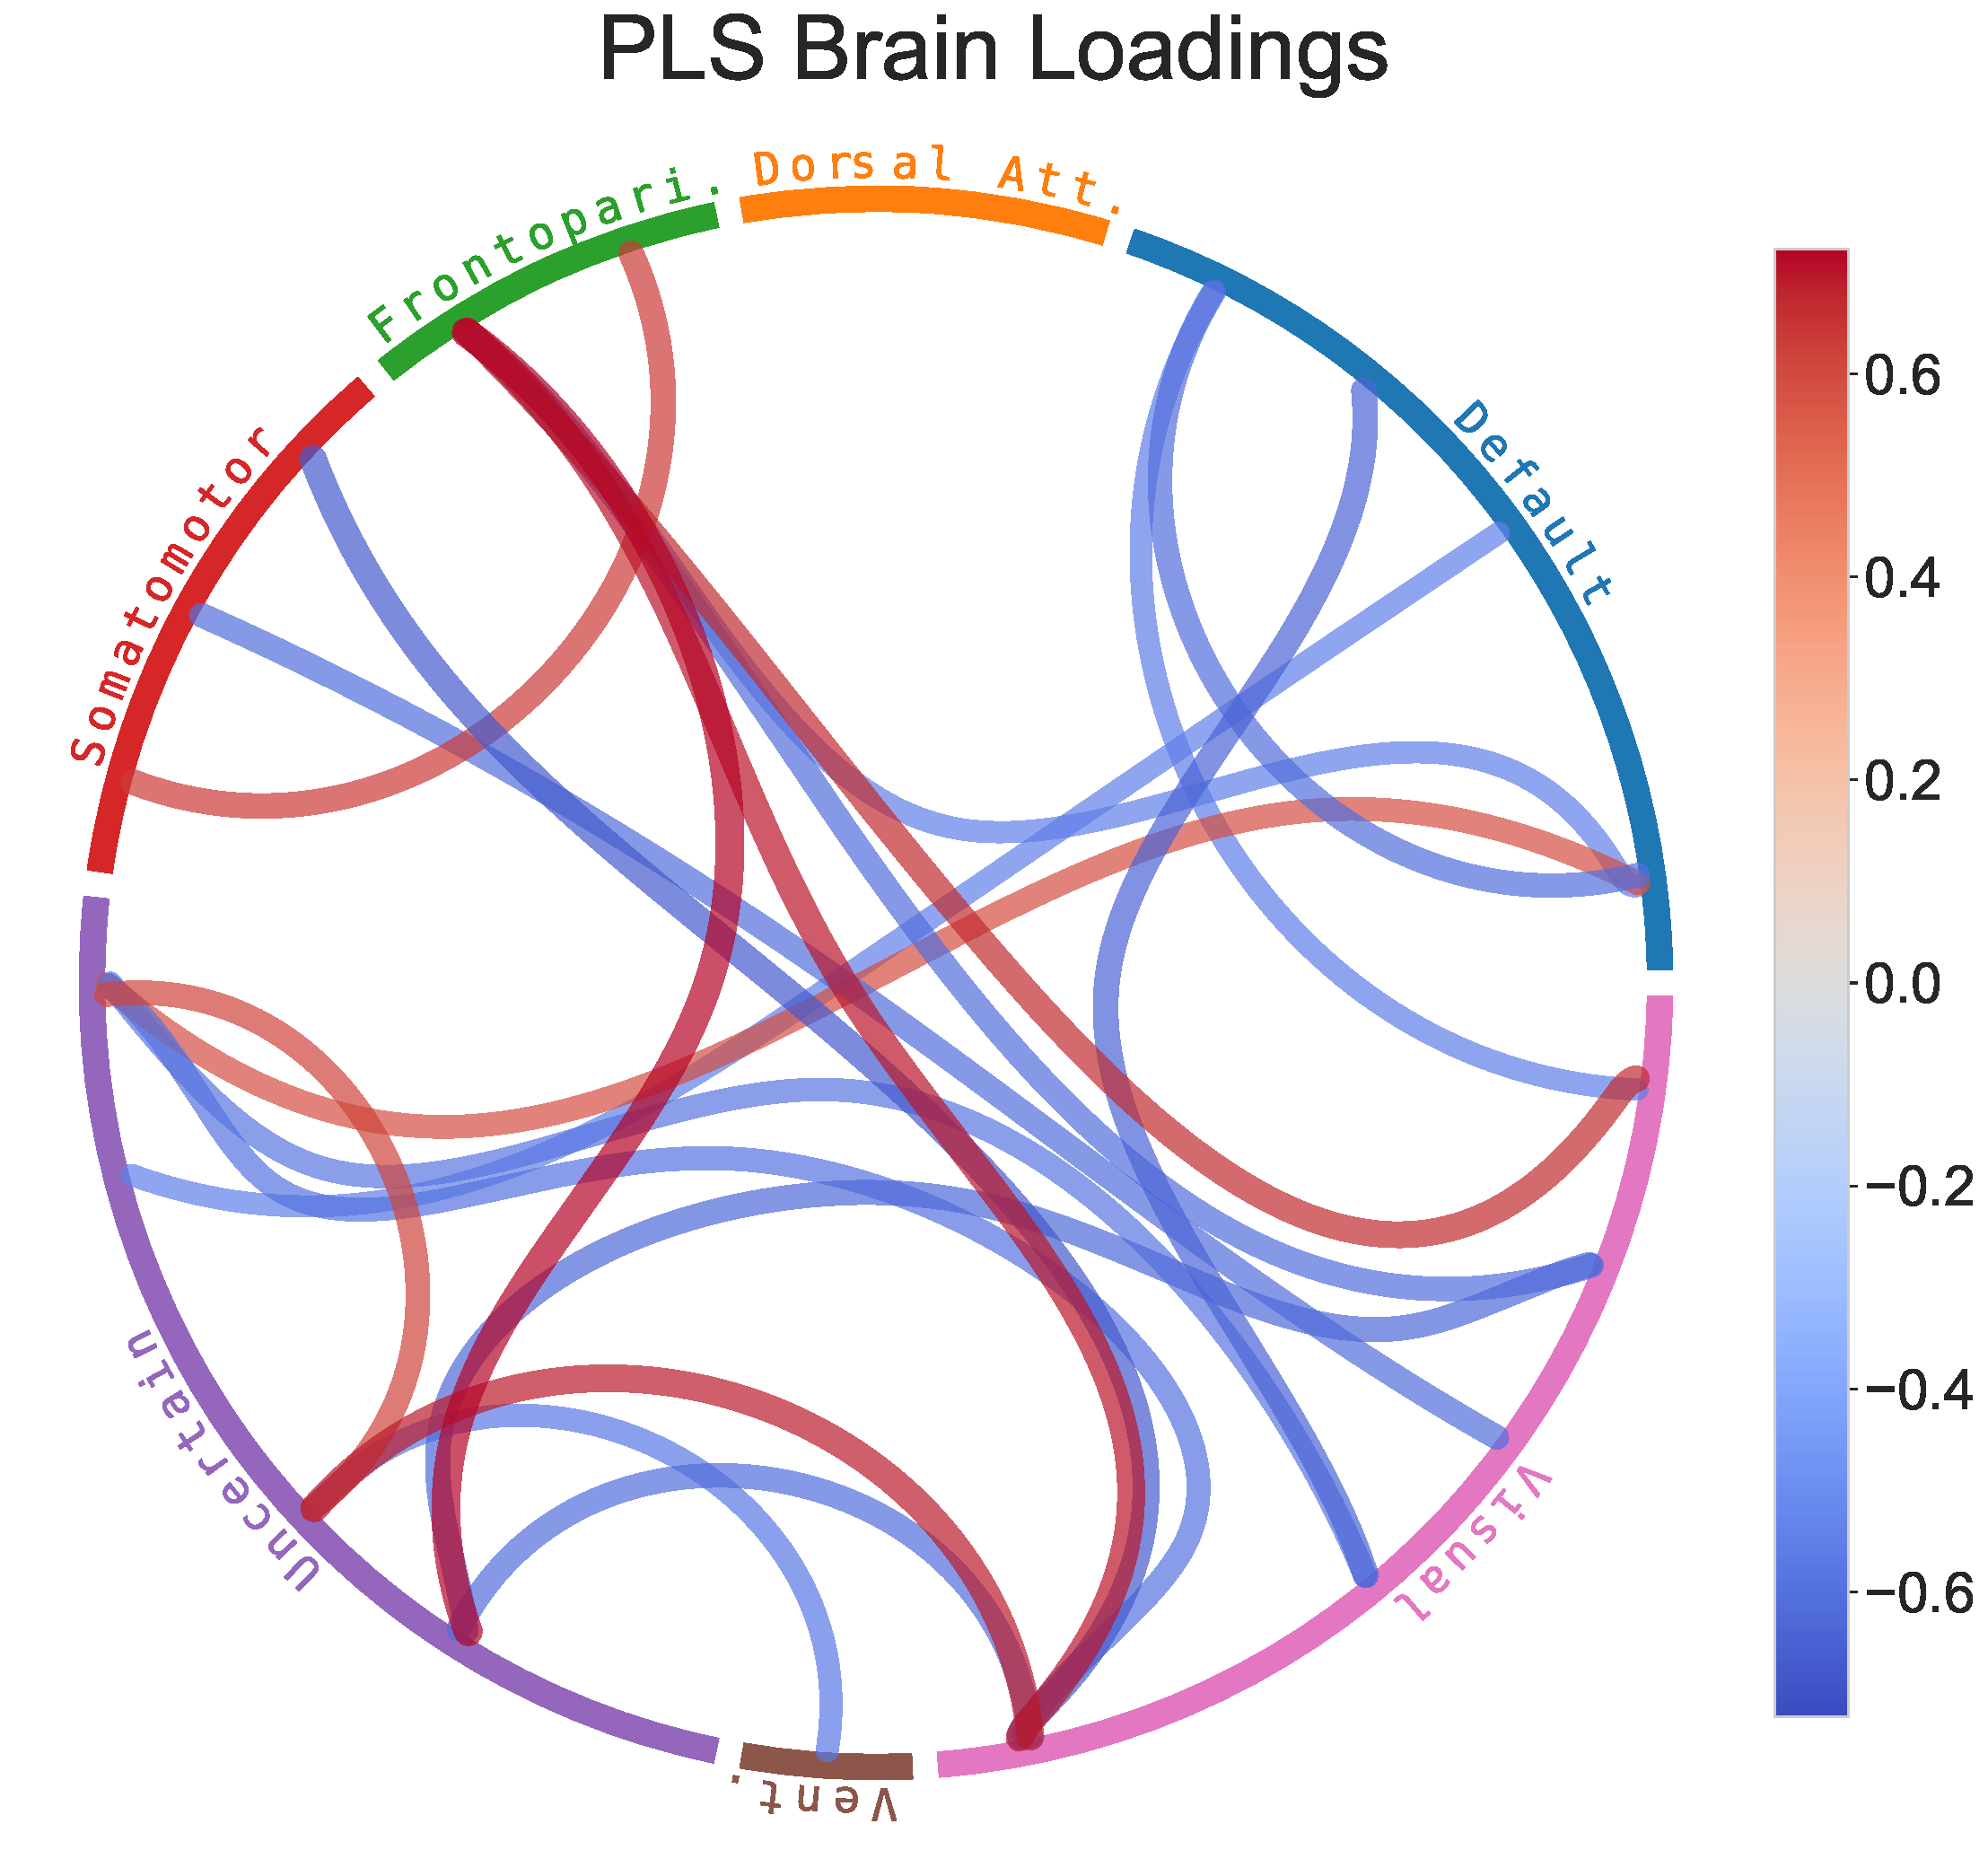
\includegraphics[width=0.68\linewidth]{figures/regularization/hcp/PLS brain loadings.pdf}
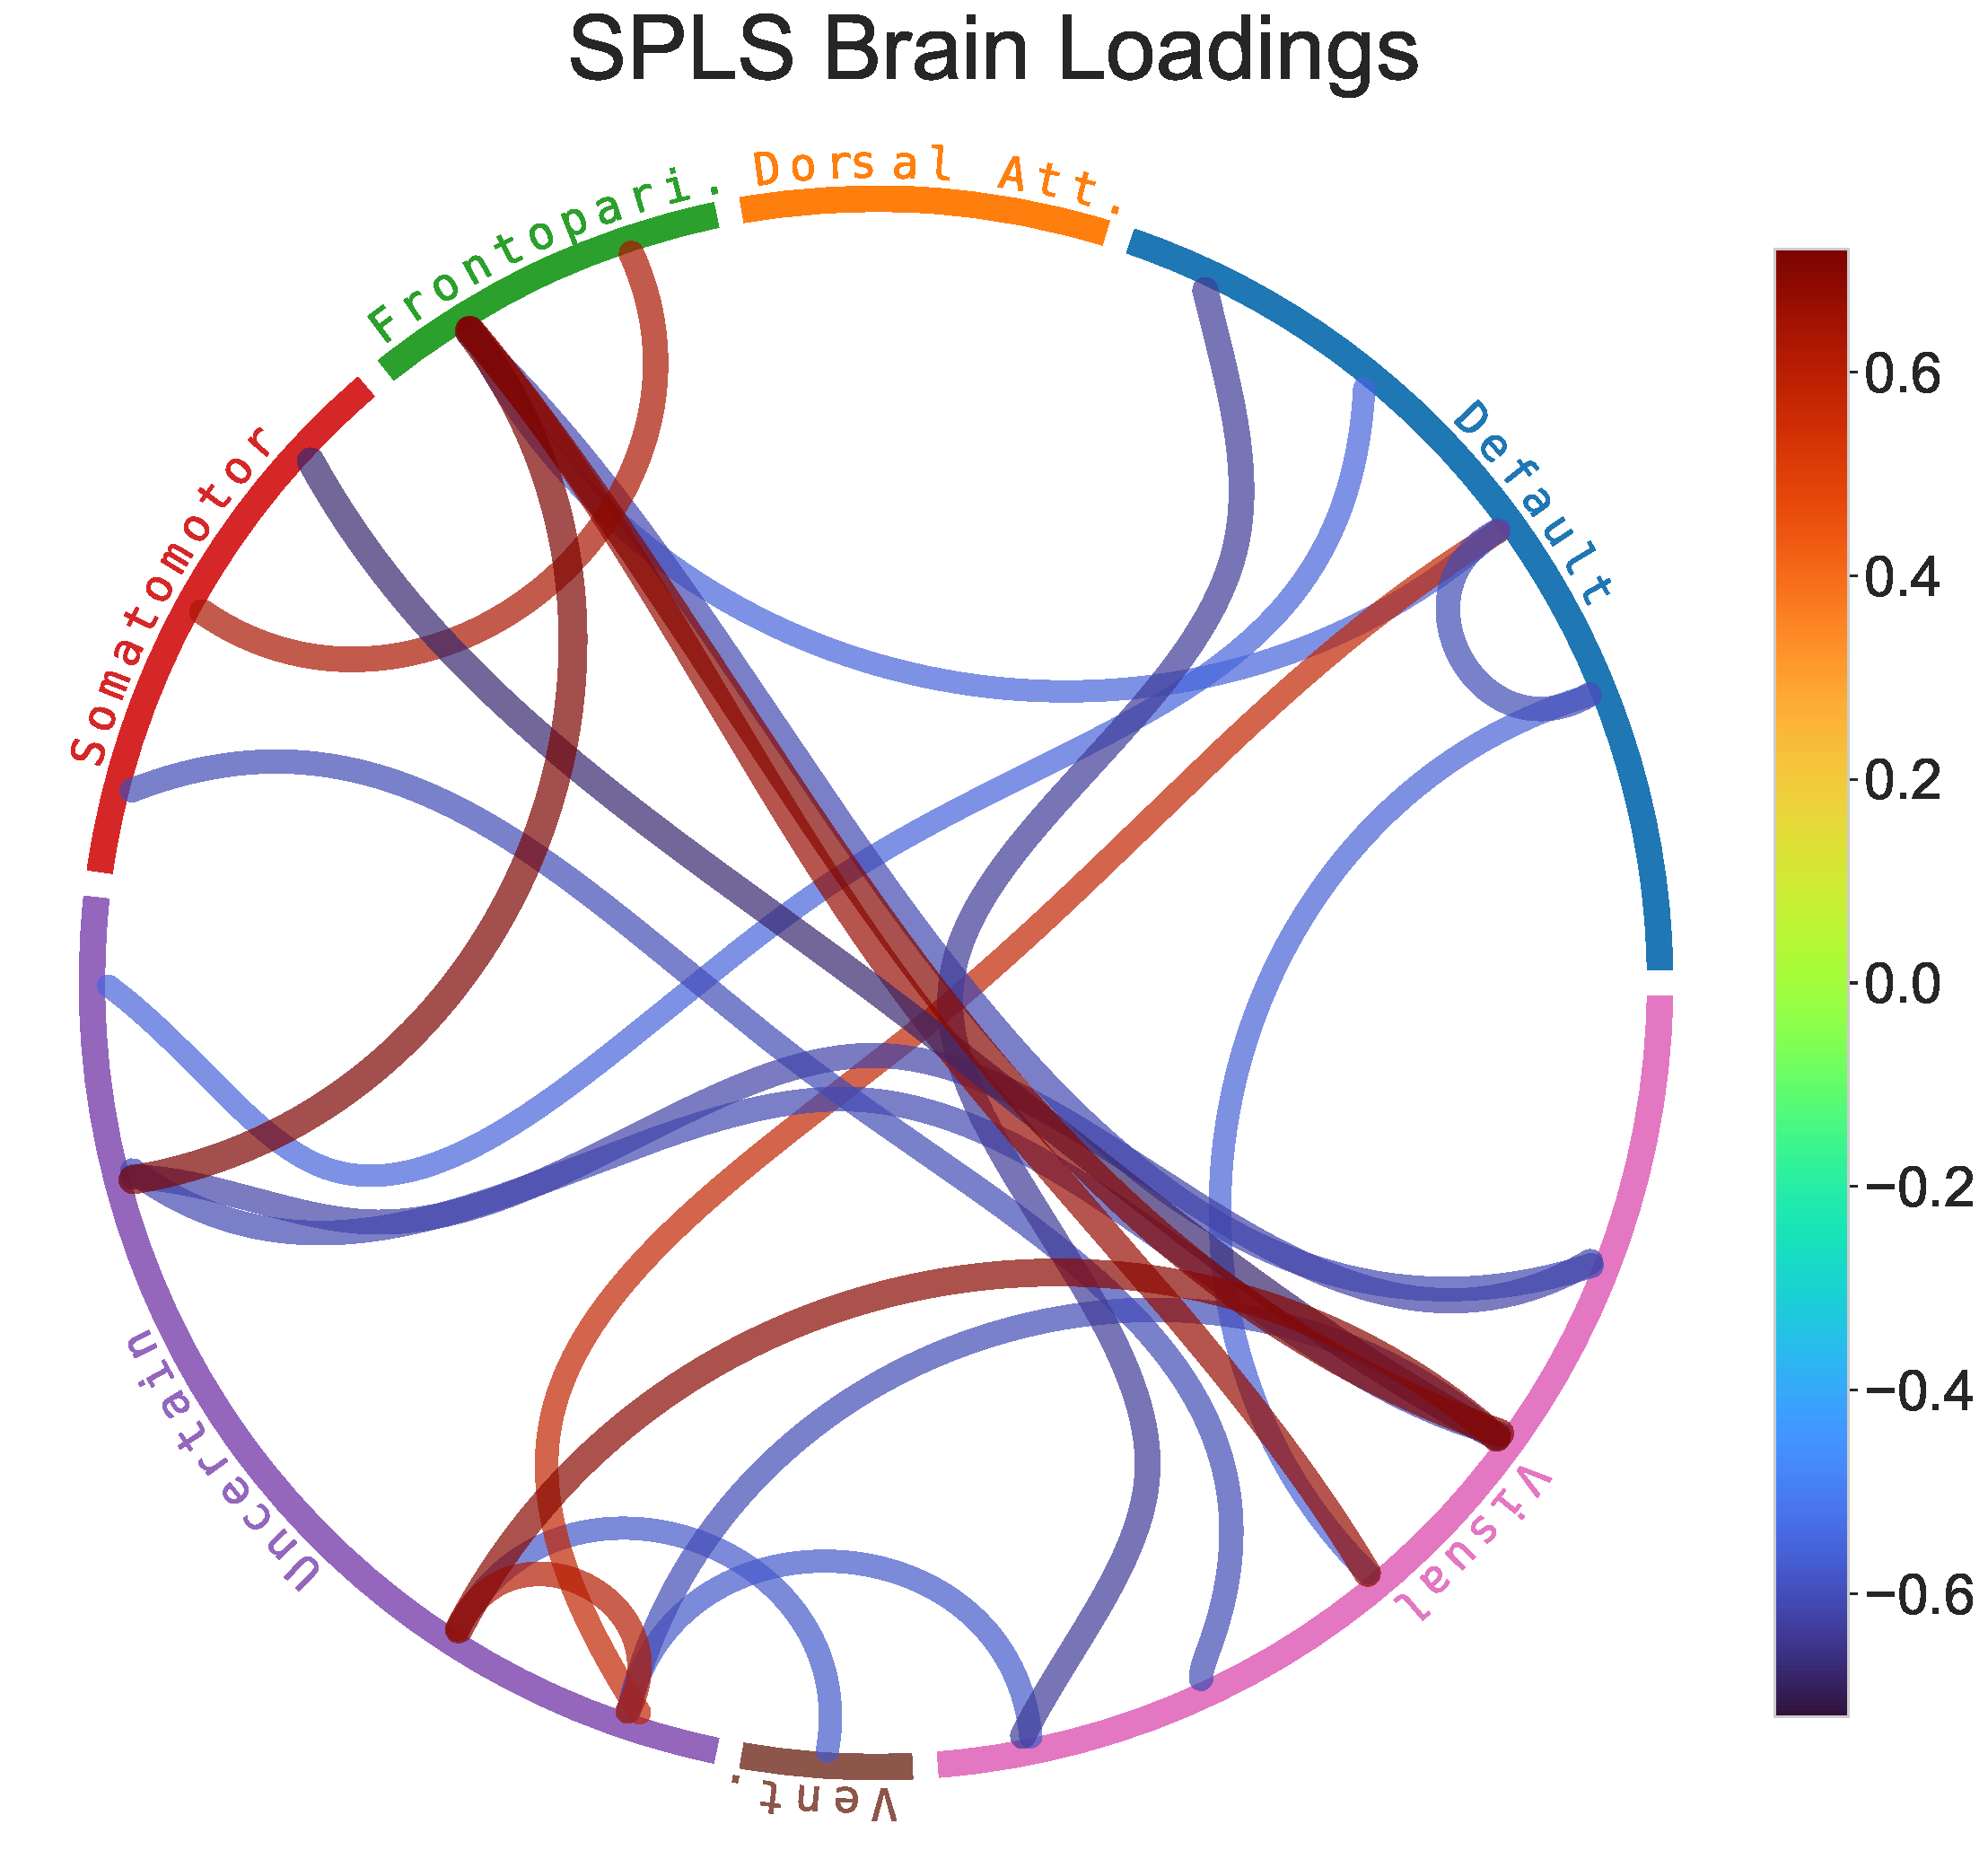
\includegraphics[width=0.68\linewidth]{figures/regularization/hcp/SPLS brain loadings.pdf}
\caption{Map of CCA connection strength variations, with each node’s parcel map weighted by CCA edge-strength changes across edges involving that node.}\label{fig:brain}
\end{figure}


\paragraph{Sparsity of Weights} Something about the sparsity of weights

\begin{table}[h]
\centering
\caption{Number of non-zero weights for each model.}
\begin{tabular}{|l|c|c|}
\hline
Model &  Brain Weights &  Behaviour Weights \\
\hline
PCA        &            300 &                145 \\
RCCA       &            300 &                145 \\
ElasticNet &            241 &                 96 \\
PLS        &            300 &                145 \\
SPLS       &            118 &                 56 \\
\hline
\end{tabular}\label{table:brain-behaviour-weights}
\end{table}



\subsection{Regularized CCA with the ADNI Data}



\subsection{Measuring the Identitiness of the Covariance Matrices}

In this section, we measure the identitiness of the covariance matrices for the simulated datasets and the HCP and ADNI datasets.
The theory we developed in section~\ref{subsec:generative-perspectives-on-cca} suggests that the identitiness of the covariance matrices is crucial for understanding how imposing sparsity on the weights imposes a prior belief in sparsity on the more biologically interesting loadings.
We measure the identitiness of the covariance matrices by looking at the eigenvalues of the covariance matrices.
If the eigenvalues of the sample covariance matrix are all close to 1, then the sample covariance matrix is close to identity.
Departures from 1 indicate that the sample covariance matrix is not close to identity and imply multicollinearity in the data.

In the simulated data, we can see that the joint covariance method with identity covariance matrices, and the GFA model with an identity noise covariance matrix, have eigenvalues closer to one than the joint covariance method with random covariance matrices, and the Probabilistic CCA model with random noise covariance matrices(Figure~\ref{fig:covariance-eigenvalues-simulated}).
On the other hand, these plots (shown for 10 random samples) show that all of the sample covariance matrices depart from the ideal case, even when the true covariance matrices are identity.

\begin{figure}
\centering
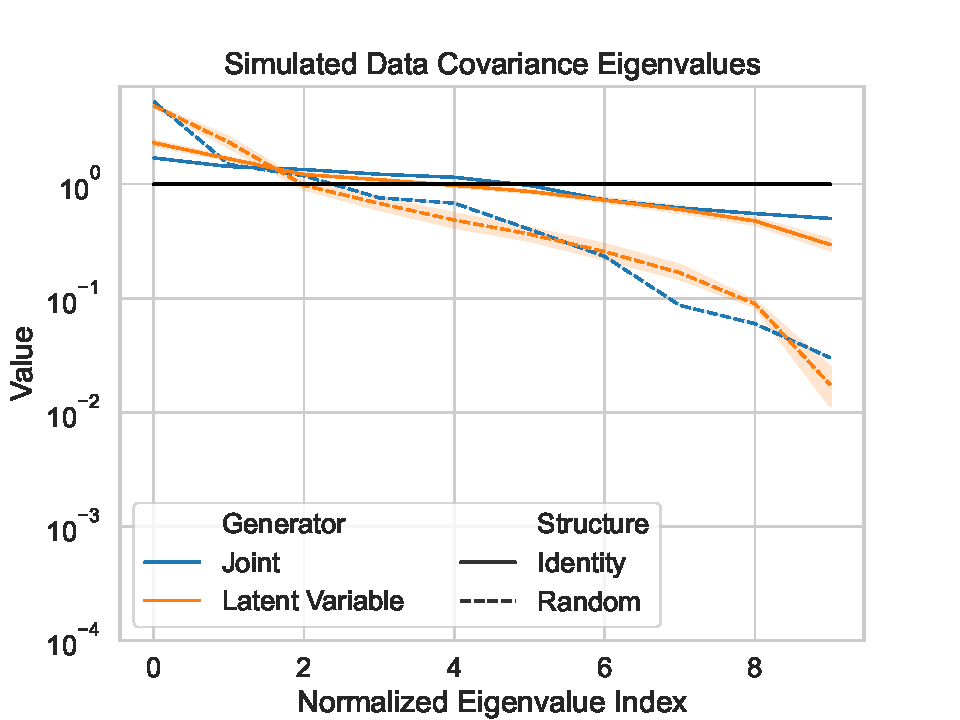
\includegraphics[width=0.8\linewidth]{figures/regularization/covariance/simulated_covariance_eigenvalues.pdf}
\caption{Eigenvalues of the covariance matrices for the simulated datasets.}\label{fig:covariance-eigenvalues-simulated}
\end{figure}

In the HCP and ADNI datasets, we can see that the only dataset and view with eigenvalues close to 1 is the ADNI brain data (Figure~\ref{fig:covariance-eigenvalues}).
This suggests that the only dataset and view where we can expect sparsity on the weights to imply sparsity on the loadings is the ADNI brain data.

\begin{figure}
\centering
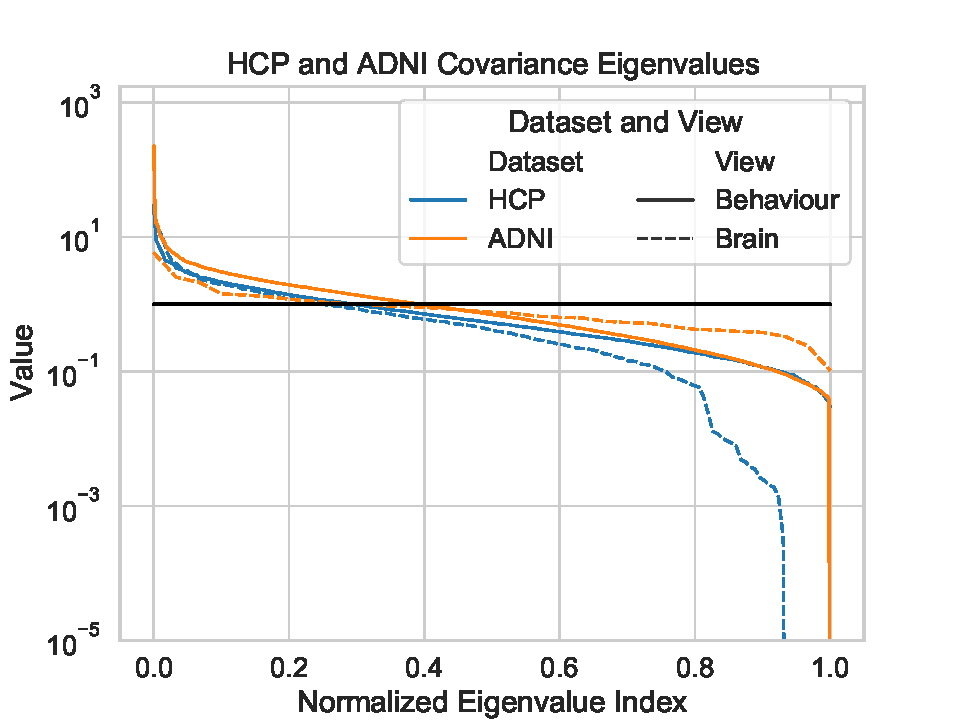
\includegraphics[width=0.8\linewidth]{figures/regularization/covariance/hcp_adni_covariance_eigenvalues}
\caption{Eigenvalues of the covariance matrices for the HCP and ADNI datasets.}\label{fig:covariance-eigenvalues}
\end{figure}

We can also see these differences by plotting the covariance matrices themselves in Figure~\ref{fig:covariance-matrices}.
In the behavioural data, which is somewhat low dimensional in both datasets, we can see the block structure of the covariance matrices.
In the brain data, we are unable to plot the whole covariance matrix because it is too high-dimensional and therefore only show a sample.


\begin{figure}
\centering
\begin{subfigure}{0.49\linewidth}
\centering
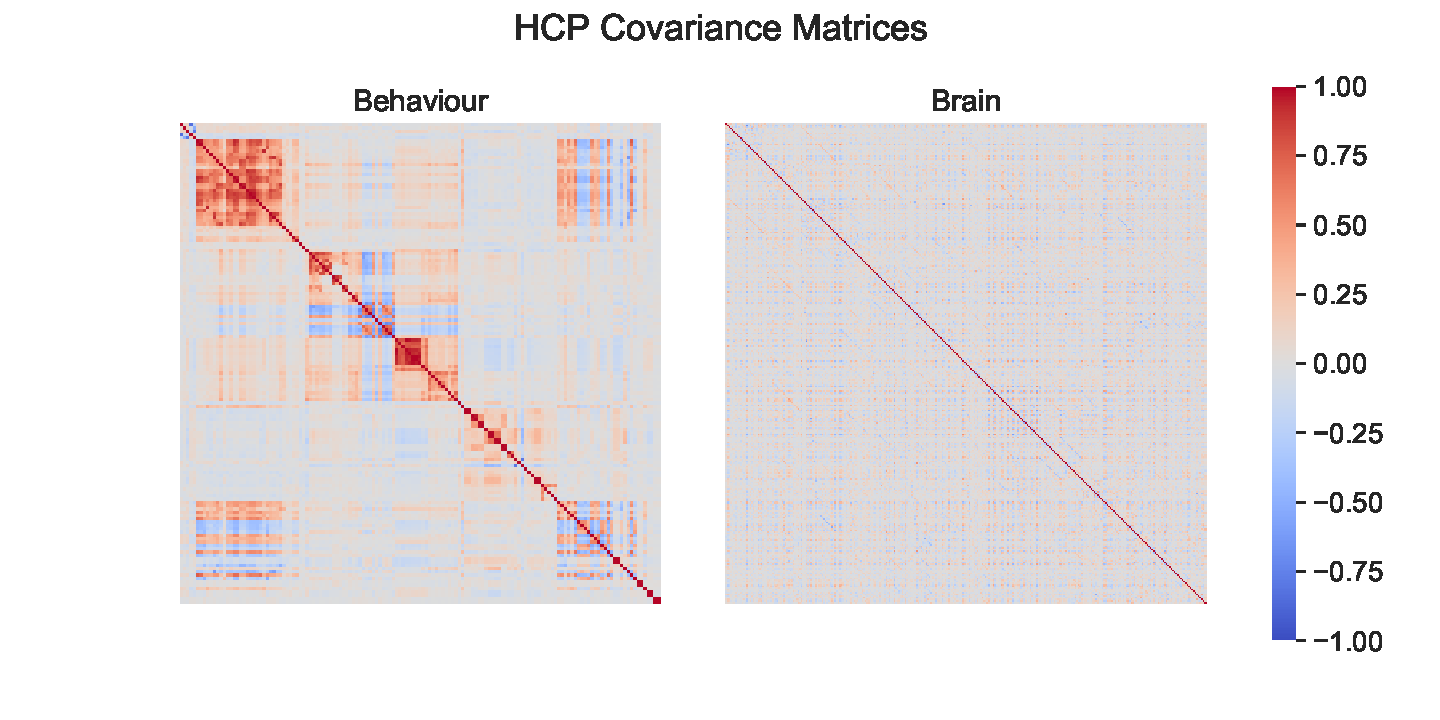
\includegraphics[width=\linewidth]{figures/regularization/covariance/HCP_covariance}
\caption{HCP}
\end{subfigure}
%
\begin{subfigure}{0.49\linewidth}
\centering
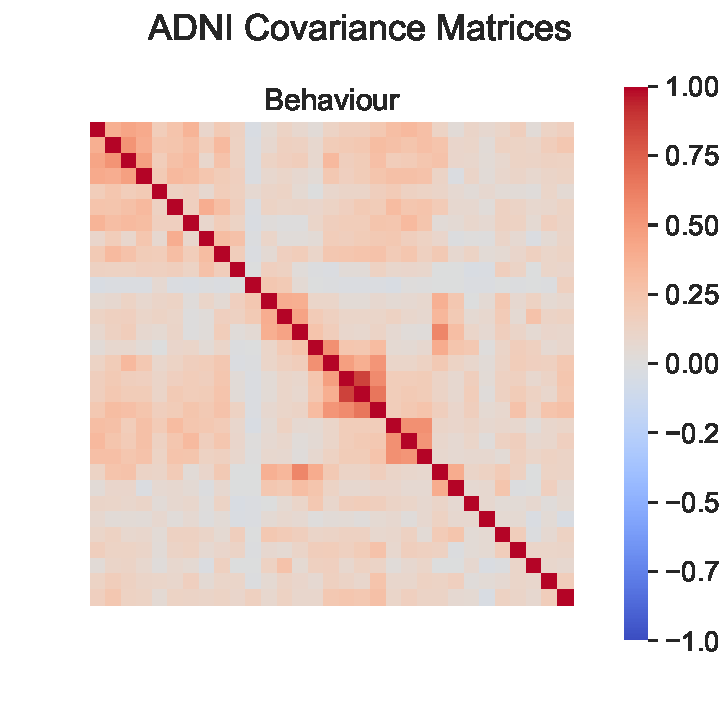
\includegraphics[width=\linewidth]{figures/regularization/covariance/ADNI_covariance}
\caption{ADNI}
\end{subfigure}
\caption{Covariance matrices for the HCP and ADNI datasets.}
\label{fig:covariance-matrices}
\end{figure}

\section{Discussion and Limitations}

In this section, we discuss the implications of our findings as well as the limitations of our approach; some of which we address in later chapters of this thesis.

\subsection{Discussion}

In this section, we outline several crucial points that emerged from our study, highlighting the considerations when using CCA and its related methods.

\subsubsection{The importance of matching the model to the data generating process}

The results showcase clear discrepancies when the underlying model does not align with the data generation process. For instance, in the \textit{Probabilistic CCA with Random Covariance Matrices} experiment, both Elastic regularization and SPLS did not enhance the performance of CCA and PLS, respectively.
This happened primarily because the real weights weren't sparse, leading to a mismatch between the model and the data generation mechanism.
These findings underscore the necessity of selecting models that mirror the intrinsic structure and nature of the data.
Inaccurate model selection can result in suboptimal outcomes, even with sophisticated regularization techniques in place.

\subsubsection{Sample versus population settings can lead to different outcomes}

The results from the \textit{Joint Covariance and Sparse Weights} experiment exemplify the disparities that can arise between population and sample settings.
Although PLS, RCCA, and CCA are equivalent under isotropic noise in a population framework, their performance can vary substantially in a sample setting.
This phenomenon exemplifies the inherent challenges that can arise when interpreting outcomes in sample settings.
It's therefore crucial for researchers to recognize these nuances and adopt appropriate measures when extrapolating results, particularly because in brain-behaviour studies, we only have one sample and its size is often limited.

\subsubsection{FRALS allows for flexible regularization for closer model matching}

Our results show that when true weights are sparse and maximal ridge regularization is not needed (i.e. SPLS), FRALS with elastic net regularization can be much more effective at recovering the true weights in simulated data.

\subsubsection{Sparsity on the weights does not imply sparsity on the loadings}

On the other hand, our results raise the question of whether sparsity on the weights makes sense in the first place.
For latent variable models of brain-behaviour associations, we have argued that the loadings are the more biologically relevant quantity.
Since in practice identity covariance is rarely a good assumption, the weights and loadings are not equivalent.
This means that sparsity on the weights does not imply sparsity on the loadings and so we should not expect sparsity on the weights to lead to more interpretable loadings.
A practical step this implies is \textit{to ensure that the data covariances are at least close to identity before applying sparse CCA methods}.

\subsubsection{ElasticNet finds a subtly different mode to other models in the HCP data}

RCCA and ElasticNet gave more weight to the parietal lobe than PCA and PMD did.
This suggests that our model finds the parietal lobe more relevant for capturing brain-behaviour correlations.
PMD focused on principal components in the brain.
This could mean PMD might miss the true associations between views.
In this setting, ElasticNet functions similarly to a sparse RCCA.

\subsection{Limitations}
While FRALS offers promising performance in terms of out-of-sample correlation, it does come with significant drawbacks, the most noteworthy being its computational inefficiency.
Below, we outline the primary factors contributing to the slow speed of FRALS and provide some insights into the computational bottlenecks.

\subsubsection{Computational Time}\label{subsec:computational-time}
While computationally intensive, the flexibility of FRALS allows it to adapt better to the complexity inherent in real-world data sets, such as the HCP. This adaptability could be crucial when high predictive accuracy or interpretability is required.

\subsubsection{Changing Regression Targets}\label{subsec:changing-regression-targets}
Adding to the computational burden is the fact that the regression targets, i.e., the projections of the other view, are not static but change dynamically throughout the algorithm's run.
Each update to the least squares solution consequently alters the global objective, leading to a constantly shifting landscape that the algorithm needs to navigate.

\section{Conclusions}

We delved into the relationship between CCA's backward and forward models.
Our findings suggest that the backward model's weights don't guarantee sparsity in the forward model's loadings.
Therefore, looking at the loadings might offer more meaningful biological insights.

We also introduced and incorporated elastic net regularization using alternating least squares to improve CCA model regularization.

We used simulated data to shine light on the challenges of interpreting the results of CCA studies, even when we know the true data generation process.
We showed the effect of different regularization techniques, the population and sample settings, loadings and weights.
We also showed clearly that PLS behaves as a heavily regularised version of CCA and is often inappropriate.
SPLS is similarly flawed despite its popularity.

In the real Brain-Behaviour data from the Human Connectome Project, we found that ...

In summary, our study underscores the need to choose the right model for specific data situations.
%
%\chapter{Gradient Descent: Accelerating CCA for Large Datasets}\label{ch:gradient_descent}
The content of this chapter is based on a preprint paper where I am first author.
I initiated the project based on heuristic arguments and contacted coauthors Ana Lawry Aguila (who provided and analysed the UK Biobank data) and Lennie Wells (who provided extensive mathematical proofs which are in the appendix of this PhD thesis for the interest of the reader).
Both of my coauthors helped me to revise the manuscript.
\minitoc

\section{Introduction}

Subspace learning techniques such as Canonical Correlation Analysis (CCA) have been essential tools in various scientific domains.
While these techniques are powerful, they face computational and scalability challenges, particularly for large datasets.
The focus of this chapter is to explore methods to effectively implement CCA using gradient descent and further scale it using stochastic gradient descent.
This chapter serves as a foundation for the application of proximal gradient descent in regularisation, which will be discussed in subsequent chapters.

\subsection{Problem Statement}

The existing methodologies for solving Canonical Correlation Analysis (CCA) face severe computational limitations, especially for large-scale datasets.
The challenges include high computational intensity and memory demands.

\subsection{Contributions}


\begin{itemize}
  \item Proposing an effective approach to solve CCA using gradient descent, laying the groundwork for future regularisation techniques using proximal gradient descent.
  \item Introducing a scalable methodology for applying CCA to large-scale medical datasets through stochastic gradient descent.
  \item Demonstrating the framework's effectiveness and scalability across diverse tasks and datasets.
  \item Providing a unique real-world application of stochastic PLS on an extremely high-dimensional biomedical dataset.
\end{itemize}

The subsequent sections will elaborate on these contributions, validating our approaches through various experimental setups and real-world applications.


\section{Background}
\subsection{Stochastic Approaches to CCA and PLS}

To the best of our knowledge, the state-of-the-art in Stochastic PLS and CCA are the subspace Generalized Hebbian Algorithm (\textbf{SGHA}) of \cite{chen2019constrained} and \textbf{$\gamma$-EigenGame} from \cite{gemp20,gemp2021}. Specifically, SGHA utilizes a Lagrange multiplier heuristic along with saddle-point analysis, albeit with limited convergence guarantees. EigenGame focuses on top-k subspace learning but introduces an adaptive whitening matrix in the stochastic setting with an additional hyperparameter.

\subsection{Reconstruction perspective on PCA and CCA}
The key idea behind this chapter relies on treating CCA as a low-rank approximation problem, rather than a constrained optimization problem or a generalized eigenvalue problem.

While this perspective is unusual in the context of CCA, it is well-known in the context of PCA. Indeed, the Eckart-Young-Mirsky theorem \cite{stewart_matrix_1990} states that the best rank-$k$ approximation to a matrix $M$ is given by the truncated SVD:

\begin{align}
    \argmin_{\substack{W \in \R^{d \times k} \\ W^T W = I}} \| M - W W^T M \|_F^2 = U_k \Sigma_k V_k^T
\end{align}

where $U_k \Sigma_k V_k^T$ is the truncated SVD of $M$. If we consider the case where $M=XX^T$, then this is precisely the PCA problem. 

This is a well-known result in matrix analysis, and it is often used to motivate PCA as a low-rank approximation problem. 
This reconstruction perspective is also the basis behind the Autoencoder, a popular deep learning architecture \cite{goodfellow2016deep}, which can be seen as a non-linear generalisation of PCA. 

In this chapter, we will show that a similar result holds for CCA and Generalized Eigenvalue Problems more generally, and that this can be used to motivate a new formulation of CCA as a low-rank approximation problem.


\section{Contributions}

In this section, we introduce a new class of algorithms based on matrix analysis results which allow us to efficiently solve a number of interesting problems including but not limited to CCA, PLS, DCCA, and SSL.

\subsection{GEP-GHA}
First, we present GEP-GH.

\begin{restatable}[Eckhart-Young inspired objective for GEPs]{proprep}{GHAcharac}
    \label{prop:GHA-charac}
    The top-$k$ subspace of the GEP $(A,B)$ can be characterised by maximising the following objective over $W \in \R^{d \times k}$:
    \begin{align}
        \mathcal{U}^\text{GEP-GHA}(W) \defeq \tr \left( 2\, W^T A W - \left(W^T A W\right) \left(W^T B W\right) \right)
    \end{align}
    Moreover, the maximum value is precisely $\sum_{j=1}^k \lambda_j^2$, where $(\lambda_j)$ are the generalised eigenvalues.
\end{restatable}

\subsection{Proof of Proposition \ref{prop:GHA-charac}}

\subsection{GEP-EY: an unconstrained objective for GEPs}

First, we present GEP-EY, a formulation of GEP problems by matrix analysis which permits efficient optimization by gradient descent.
This is summarised by proposition \ref{prop:EY-charac}, a consequence of applying the Eckhart-Young-Minsky inequality \cite{stewart_matrix_1990} to the eigen-decomposition of $B^\mhalf A B^\mhalf$. Detailed statements and proofs can be found in supplement \ref{supp:proofs}.

\begin{restatable}[Eckhart-Young inspired objective for GEPs]{proprep}{EYcharac}
    \label{prop:EY-charac}
    The top-$k$ subspace of the GEP $(A,B)$ can be characterised by maximising the following objective over $W \in \R^{d \times k}$:
    \begin{align}
        \mathcal{U}^\text{GEP-EY}(W) \defeq \tr \left( 2\, W^T A W - \left(W^T B W\right) \left(W^T B W\right) \right)
    \end{align}
    Moreover, the maximum value is precisely $\sum_{j=1}^k \lambda_j^2$, where $(\lambda_j)$ are the generalised eigenvalues.
\end{restatable}


In the following sections, we describe a number of algorithms for solving GEPs using proposition \ref{prop:EY-charac}.
These will be denoted with \textbf{EY} and \textbf{GHA}.

\subsection{Stochastic Optimization}

We next show how GEP-EY and CCA-SVD can be efficiently optimized using stochastic methods, which makes them suitable for large-scale and online settings.
Suppose we have an unbiased estimate $\hat{A}$ for $A$ and a pair of independent and unbiased estimates $(\hat{B},\hat{B}')$ of the matrix $B$ (for example obtained from a minibatch); then one can estimate the objective in proposition \ref{prop:constr-charac} by:
\begin{align}
    \hat{\mathcal{U}}^\text{GEP-EY}(W) \defeq \tr \left( 2\, W^T \hat{A} W - \left(W^T \hat{B} W\right) \left(W^T \hat{B}' W\right) \right)
\end{align}
which we can differentiate to give a gradient estimate:
\begin{align}\label{eq:GEP-EY-grad}
    \hat{\Delta}^{\text{GEP-EY}}(W)
    \defeq \nabla_W \hat{\mathcal{U}}^\text{GEP-EY}(W)
    % old = 4 \left\{ \hat{A} W - \hat{B} W \left(W^T \hat{B}' W \right) \right\}
    = 2 \left\{ 2 \hat{A} W - \hat{B} W \left(W^T \hat{B}' W \right) - \hat{B}' W \left(W^T \hat{B} W \right) \right\}
\end{align}

By the independence of $(\hat{B},\hat{B}')$ both of these estimates are unbiased.

The unbiased estimate immediately leads to Algorithm \ref{alg:Delta}.
The key advantage of this is that the computational complexity of the algorithm is only $\mathcal{O}(b d k)$; this is far less than the $\mathcal{O}(N d^2)$ complexity of any methods which evaluate the matrices $A,B$ on the full batch.

\textit{Why is the complexity so low?} Because $A,B$ are linear functions of covariance matrices, we can construct our unbiased estimates by plugging in sample covariances on a minibatch.
These estimates will then be low rank; indeed we can factorise these estimates in the form $\hat{M} \hat{M}^T$ where $\hat{M} \in \R^{d \times b}$. The dominant cost in evaluating $\mathcal{U}^\text{GEP-EY}$ is then just the matrix multiplications of the form $\hat{M}^T W$; see supplement \ref{supp:analyticsubspace} for full details.

\begin{algorithm}
    \caption{GEP-EY: A Stochastic Gradient Descent Algorithm for GEP subspace}
    \label{alg:Delta}
    \begin{algorithmic}
        \STATE {\bfseries Input:} data stream $Z_t$ consisting of B samples from $z_n$. Learning rate $(\eta_t)_t$. Number of time steps $T$. Number of eigenvectors to compute $k$.
        \STATE {\bfseries Initialise:} $(\hat{\mathbf {W}})_{i=1}^K$ with random uniform entries
        \FOR{$t=1$ {\bfseries to} $T$}
        \STATE Construct an independent unbiased estimate of $\hat{A}$ and two independent unbiased estimates of $\hat{B}$ from $Z_t$
        \STATE $\hat{\mathbf {W}} \leftarrow \hat{\mathbf {W}}+\eta_{t} \hat{\Delta}^{\text{GEP-EY}}$
        \COMMENT{As defined in (\ref{eq:GEP-EY-grad})}
        \ENDFOR
    \end{algorithmic}
\end{algorithm}

%%%%%%%%%%%%%%%%%%%%%%%%%%%%%%%%%%%%%%%%%%%%%%%%%%%%%%%%%%%%%%%%%%%%%%%%%%%%%%%%%%%%%%
%Stochastic CCA
%%%%%%%%%%%%%%%%%%%%%%%%%%%%%%%%%%%%%%%%%%%%%%%%%%%%%%%%%%%%%%%%%%%%%%%%%%%%%%%%%%%%%%
\section{Experiment 1: Application of CCA-EY to stochastic CCA}

\subsection{Experiment Design}

\subsubsection{Data}
\textbf{Mediamill}: The MediaMill dataset \cite{feng2004context} is a benchmark dataset for multilabel classification
. It consists
of 1200 video clips from the TRECVID 2003 conference, each annotated with 101 labels. The original goal of the dataset was to predict the labels of the videos from the visual and audio features. It has since become a benchmark dataset for CCA and other multiview learning methods. We use the same features as \cite{gemp2022generalized} which are 128-dimensional bag-of-visual-words features and 13-dimensional bag-of-audio-words features. We split the data into 80\% train and 20\% test and use cross-validation within the training data in order to tune hyperparameters.

\textbf{Split CIFAR}: The CIFAR-10 dataset \cite{krizhevsky2009learning} consists of 60,000 32x32 colour images in 10
classes, with 6000 images per class. There are 50,000 training images and 10,000 test images. We split the images into two halves.

In this section, we compare GEP-GD and CCA-SVD to $\gamma$-EigenGame \cite{gemp2022generalized} and SGHA \cite{chen2019constrained} for approximating CCA in the stochastic setting. Replicating the experiment in \cite{meng2021online, gemp2022generalized}, we optimize for the top-4 CCA subspace for the MediaMill and Split CIFAR (left and right halves of CIFAR-10 images) datasets. We use a minibatch size 100 and train for one epoch across 5 random seeds (with 1 standard deviation error bars in the plots). We use the Scipy \cite{virtanen2020scipy} package to solve the full batch GEPs as a ground truth value and use the proportion of correlation captured (PCC) captured by the learnt subspace as compared to this ground truth (defined in supplement \ref{supp:experimental details}). Unlike \cite{gemp2022generalized}, we do not perform PCA on the data before applying the CCA methods but instead, for the MNIST data, we add gaussian noise to avoid zero variance subspaces in $X$ and $Y$. This makes our task more challenging, as performing PCA simplifies the problem by substituting $B$ for the identity matrix $I$. This explains the decrease in performance of $\gamma$-EigenGame as compared to their original work.


\subsection{Results}

Figure \ref{fig:ccaiter} shows that both of our methods outperform SGHA and $\gamma$-EigenGame on both datasets in terms of speed of convergence and achieve near-optimal performance in terms of PCC after just one epoch. All of the algorithms share the same complexity per iteration so that these results are also representative in terms of runtime. This demonstrates the effectiveness and superiority of our method for solving CCA in the stochastic setting.

\begin{figure}%[H]
    \centering
    \begin{subfigure}[b]{0.49\textwidth}
        \centering
        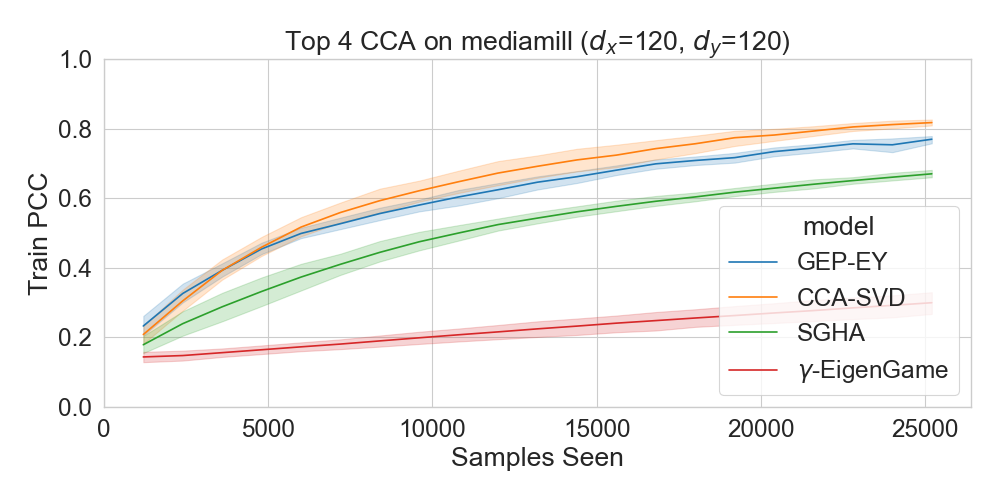
\includegraphics[width=\textwidth]{figures/gradient_descent/CCA/mediamill_100_pcc_lr_tuned.png}
        \label{fig:ccamediamill}
    \end{subfigure}
    \hfill
    \begin{subfigure}[b]{0.49\textwidth}
        \centering
        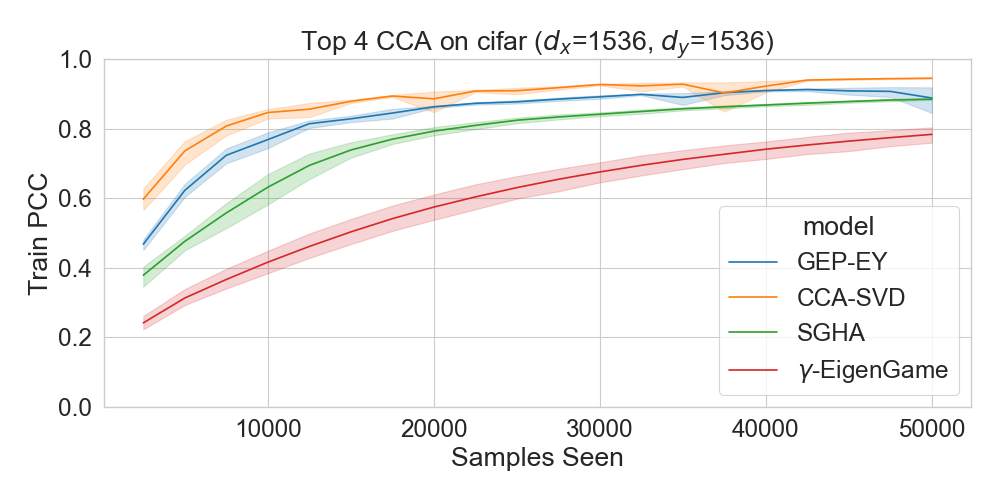
\includegraphics[width=\textwidth]{figures/gradient_descent/CCA/cifar_100_pcc_lr_tuned.png}
        \label{fig:ccacifar}
    \end{subfigure}
    \caption{PCC with respect to Scipy ground truth by GEP-EY and CCA-SVD vs prior work for (a) MediaMill and (b) Split CIFAR data. The maximum value is 1.0 and shading represents $\pm$ 1 standard deviation.}
    \label{fig:ccaiter}
    \label{fig: stochasticcca}
\end{figure}

\subsubsection{Stochastic CCA Minibatch Size}
In this section, we take a closer look at how minibatch sizes impact the performance of our method in the stochastic CCA setting. We maintain a constraint of single epoch training. This means that when we use smaller minibatches, the number of training steps increases correspondingly.

Our experiments, as displayed in Figure \ref{fig:minibatch size ablation}, show that our method performs well across a range of minibatch sizes. Notably, it achieves high performance even when the minibatch size is nearly equivalent to the number of components.

This indicates that our method can learn effectively from a limited number of samples. It suggests the possibility of applying our method to analyse large datasets on devices with restricted memory, by processing small minibatches of data sequentially. This robustness to minibatch size could potentially make our method a viable solution for large-scale data analysis where computational resources are limited.

\begin{figure}[h]
    \centering
    \begin{subfigure}[b]{0.49\textwidth}
        \centering
        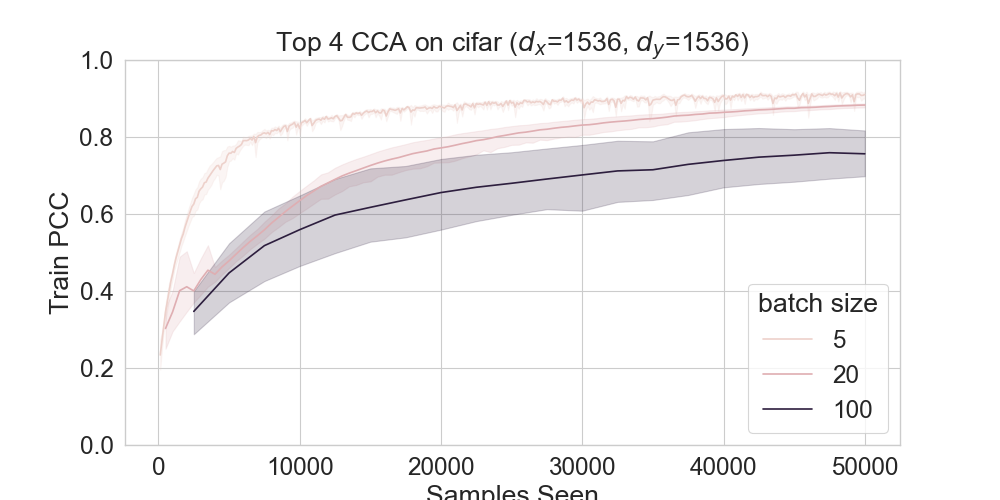
\includegraphics[width=\textwidth]{figures/gradient_descent/CCA/cifar_minibatch_size_ablation.png}
        \caption{}
        \label{fig:cifar_minibatch_ablation}
    \end{subfigure}
    \begin{subfigure}[b]{0.49\textwidth}
        \centering
        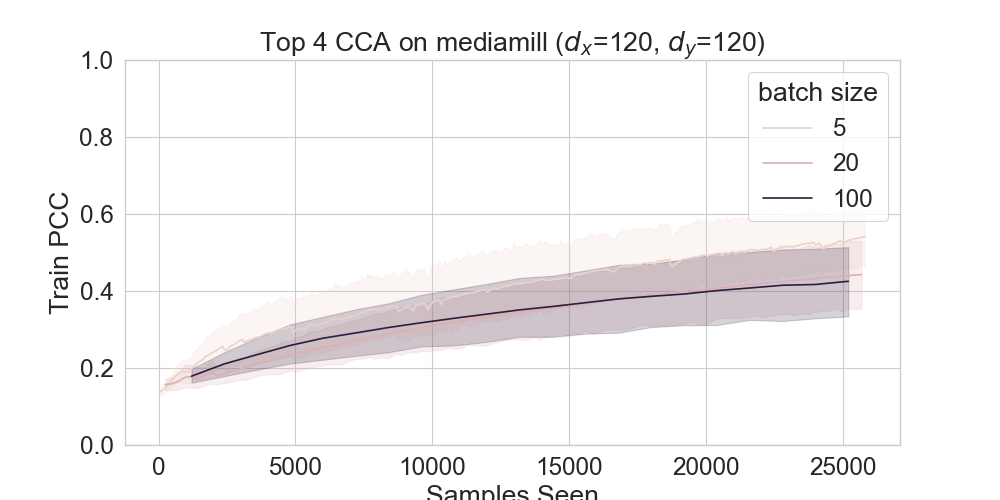
\includegraphics[width=\textwidth]{figures/gradient_descent/CCA/mediamill_minibatch_size_ablation.png}
        \caption{}
        \label{fig:mediamill_minibatch_ablation}
    \end{subfigure}
    \caption{Ablation study on minibatch size for stochastic CCA for (a) cifar and (b) mediamill datasets for minibatch sizes 100, 20, and 5}
    \label{fig:minibatch size ablation}
\end{figure}

\subsection{Discussion}



%Stochastic PLS UKBB
%%%%%%%%%%%%%%%%%%%%%%%%%%%%%%%%%%%%%%%%%%%%%%%%%%%%%%%%%%%%%%%%%%%%%%%%%%%%%%%%%%%%%%
\section{Experiment 2: Application of PLS-EY to PLS on large scale biomedical data}

\subsection{Experiment Design}

\subsection{Data}
\textbf{The UK Biobank}: is arguably the largest scale biomedical database in the world with around half a
million
total participants. The goal is to have imaging data for the brain, heart, and body for 100,000 participants. The UK Biobank combines these images with genetics, biomarkers, electronic health record, and online questionnaires making it a rich dataset for broad studies of health.

For the GEP-EY PLS analysis on biomedical data, we used 33,333 subjects from the UK Biobank \cite{sudlow2015uk}. We used pre-processed (using FreeSurfer \cite{Fischl2012}) grey-matter volumes for 66 cortical (Desikan-Killiany atlas) and 16 subcortical brain regions and 582,565 autosomal genetic variants. The affects of age, age squared, intracranial volume, sex, and the first 20 genetic principal components for population structure were removed from the brain features using linear regression to account for any confounding effects. Each brain ROI was normalised by removing the mean and dividing the standard deviation. We processed the genetics data using PLINK \cite{Purcell2007} keeping genetic variants with a minor allele frequency of at least 1\%  and a maximum missingness rate of 2\%. We used mean imputation to fill in missing values and centered each variant.

To generate measures of genetic disease risk, we calculated polygenic risk scores using PRSice \cite{PRSice2014}. We calculated scores, with a p-value threshold of 0.05, using GWAS summary statistics for the following diseases; Alzheimer's \cite{Lambert2013}, Schizophrenia \cite{Trubetskoy2022}, Bipolar \cite{Mullins2021}, ADHD \cite{Demontis2023}, ALS \cite{Van_Rheenen2021}, Parkinson's \cite{Nalls2019}, and Epilepsy \cite{International_League_Against_Epilepsy_Consortium_on_Complex_Epilepsies2018}, using the referenced GWAS studies.

We demonstrate the power of GEP-EY for large-scale subspace learning by solving PLS on imaging genetics data from the UK Biobank \cite{sudlow2015uk}, a biomedical database.
This can reveal novel phenotypes of interest and uncover genetic mechanisms of disease and brain morphometry.
Previous imaging genetics analyses using PLS and CCA were limited to small-scale datasets \cite{Lorenzi2018,Taquet2021,Lefloch2012}, which are prone to overfitting and instability.
Full batch approaches are infeasible for this data due to the high computational cost.
The only other large-scale PLS analysis on the UK Biobank used a federated approach with local batch PLS-SVD \cite{lorenzi2016}, which approximates the global solution.
We present the first stochastic PLS analysis on large-scale biomedical data.

We ran GEP-EY with minibatch size 500 on brain imaging (82 regional volumes) and genetics (582,565 variants) data for 33,333 subjects; a massive amount of data that challenges existing methods.
See supplement (Section \ref{sec:ukbb_preprocessing}) for data pre-processing details.
We see strong validation correlation between all 10 corresponding pairs of vectors in the PLS subspace and weak cross correlation, indicating that our model learnt a coherent and orthogonal subspace of covariation (Figure \ref{fig:UKBB_corr}), a remarkable feat for such high-dimensional data.
We found that the PLS brain subspace was associated with genetic risk measures for several disorders (Figure \ref{fig:genetic_risk}), suggesting that the PLS subspace encodes relevant information for genetic disease risk, a significant finding for biomedical research.


% First Figure
\begin{figure}
    \centering
    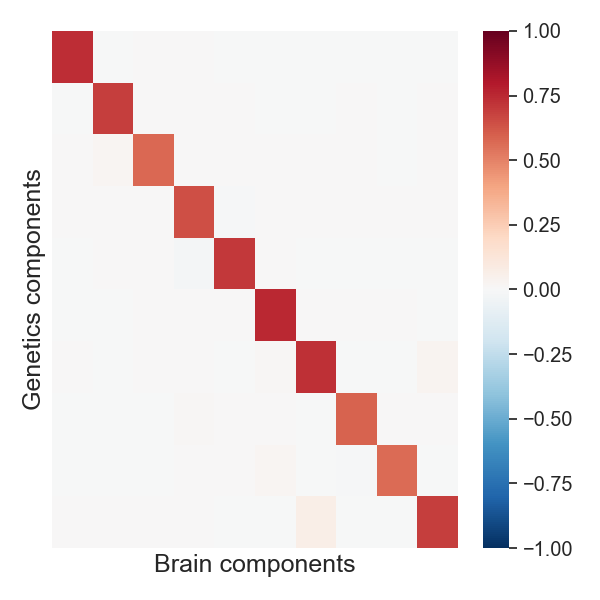
\includegraphics[width=0.5\textwidth,trim={0.8cm 0cm 0.3cm 0cm}]{figures/gradient_descent/UKBB/cross_corr}
    \caption{Correlations between PLS components for UK Biobank. This figure shows strong validation correlation between all 10 corresponding pairs of vectors in the PLS subspace and weak cross correlation, demonstrating that our model has learned a coherent and orthogonal subspace of covariation.}
    \label{fig:UKBB_corr}
\end{figure}

% Second Figure
\begin{figure}
    \centering
    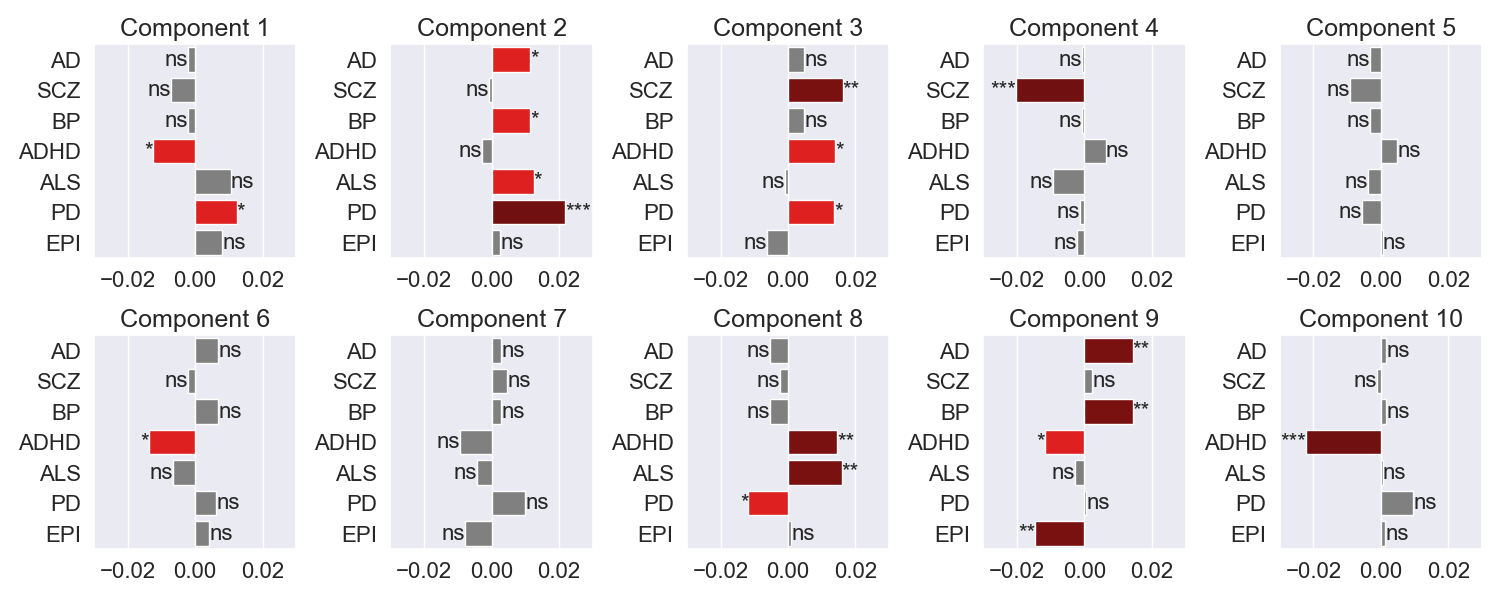
\includegraphics[width=0.7\textwidth,trim={0.5cm 0cm 0.7cm 0cm}]{figures/gradient_descent/UKBB/prs_correlations}
    \caption{Correlations between PLS brain components and genetic risk scores for several disorders. AD=Alzheimer's disease, SCZ=Schizophrenia, BP=Bipolar, ADHD=Attention deficit hyperactivity disorder, ALS=Amyotrophic lateral sclerosis, PD=Parkinson's disease, EPI=Epilepsy. The p-value significance levels are indicated as $\text{ns}: 0.05< p <= 1, \ast: 0.01< p <=0.05, \ast\ast: 0.001< p <= 0.01, \ast\ast\ast: 0.0001< p <= 0.001$. This suggests that the PLS subspace encodes relevant information for assessing genetic disease risk, an important contribution to biomedical research.}
    \label{fig:genetic_risk}
\end{figure}


\subsection{Discussion and Conclusion}

\section{Conclusion}

We presented a new unconstrained objective to characterise GEPs; this immediately gave efficient algorithms to solve many subspace learning methods in the stochastic setting with SGD.
Crucially, the gradient estimates are unbiased and cheap to compute.
Moreover, the only hyperparameter is the choice of optimiser.
We will later show how this work can be adapted and applied to optimise regularised GEPs and, in particular, CCA.

\appendix

\section{Appendix}
%
%\chapter{Proximal Gradient Descent: A Flexible, Scalable Approach to Regularised CCA}
\label{ch:proximal-gradient-descent}
\minitoc

% And this gives us the generalized eigenvalue problem~\citep{rosipal2005overview}:

% \begin{align}
%     \begin{pmatrix}
%         0 & \hat{\Sigma_{12}} \\
%         \hat{\Sigma_{21}} & 0 
%     \end{pmatrix} \begin{pmatrix}
%         u^{(1)} \\
%         u^{(2)}
%     \end{pmatrix}= \begin{pmatrix}
%         (1-c_1)\hat{\Sigma_{11}} + c_1I & 0 \\
%         0 & (1-c_2)\hat{\Sigma_{22}} + c_2I
%     \end{pmatrix}\begin{pmatrix}
%         u^{(1)} \\
%         u^{(2)}
%     \end{pmatrix}
% \end{align}

% The main difference between this eigenvalue problem and the CCA eigenvalue problem is the substitution of the matrices \(\Sigma_{11}\) and \(\Sigma_{22}\) for the matrices \( ((1-c_1) \Sigma_{11} + c_1 I) \) and \( ((1-c_2) \Sigma_{22} + c_2 I) \).
% We can therefore see that this regularisation is equivalent to adding a constant `ridge' to the diagonal of the covariance matrix \(X\spstop{i} X\sps{i}\).

\section{Introduction}

High-dimensional data are now more prevalent than ever, presenting both opportunities and challenges.
Canonical Correlation Analysis (CCA), despite its utility, struggles with high-dimensional datasets, resulting in problems like overfitting and computational inefficiency.
The CCA-EY formulation, introduced in the previous chapter, partially addresses these issues but leaves room for improvement, particularly for large-scale neuroimaging datasets.
This chapter aims to bridge this gap by incorporating regularization techniques via proximal gradient descent.

\section{Problem Statement}

The application of CCA in high-dimensional settings, such as neuroimaging data containing tens of thousands of subjects and features, often leads to overfitting.
While CCA-EY has mitigated some challenges, there remains a critical need for a methodology that can handle large-scale, high-dimensional data without sacrificing interpretability or computational efficiency.

\section{Contributions}

Our contributions in this chapter are as follows:

\begin{itemize}
    \item We integrate regularization into the CCA-EY framework to explicitly tackle the high-dimensionality problem. See \textit{Section X} for technical details.
    \item We employ proximal gradient descent to optimize the regularized objective function, creating a method that is both scalable and interpretable.
    \item A comparative analysis against existing techniques validates the effectiveness of our approach.
    \item A case study demonstrates the real-world applicability of the proposed method. Refer to \textit{Section X} for an in-depth look at the implementation and results.
\end{itemize}

In summary, this chapter introduces a robust, scalable, and interpretable extension to the CCA-EY framework to better analyze high-dimensional, multimodal data.

\section{Background}

\subsection{Proximal Gradient Descent}

Proximal Gradient Descent is an optimization algorithm commonly used for solving non-smooth convex optimization problems.
The general objective function can be expressed as \( f(x) + g(x) \), where \( f(x) \) is a differentiable convex function and \( g(x) \) is a non-differentiable convex function.
The algorithm iteratively updates \( x \) using the following equation:

\[
x^{(k+1)} = \text{prox}_{\alpha g} \left( x^{(k)} - \alpha \nabla f(x^{(k)}) \right)
\]

Here, \( \alpha \) is the step size, \( \nabla f(x^{(k)}) \) is the gradient of \( f \) at \( x^{(k)} \), and \( \text{prox}_{\alpha g}(v) \) is the proximal operator defined as:

\[
\text{prox}_{\alpha g}(v) = \arg\min_{x} \left( g(x) + \frac{1}{2\alpha} \| x - v \|^2 \right)
\]

By combining the gradients of the smooth part \( f(x) \) and the proximal operator of the non-smooth part \( g(x) \), proximal gradient descent is capable of solving problems that are otherwise intractable using basic gradient descent.

\subsection{Total Variation Regularization}

Total Variation (TV) Regularization is a regularization technique often used for signal denoising and image reconstruction. The TV norm of a signal \( x \in \mathbb{R}^n \) is given by:

\[
\| x \|_{TV} = \sum_{i=1}^{n-1} |x_{i+1} - x_i|
\]

In a 2D image, the TV norm extends to:

\[
\| x \|_{TV} = \sum_{i,j} \sqrt{(x_{i+1,j} - x_{i,j})^2 + (x_{i,j+1} - x_{i,j})^2}
\]

When incorporated as a regularizer \( R(x) \) in an optimization problem, it typically takes the form:

\[
\min_{x} \; f(x) + \lambda \| x \|_{TV}
\]

where \( \lambda \) is the regularization parameter that controls the trade-off between the data fidelity term \( f(x) \) and the regularizer \( \| x \|_{TV} \).

By leveraging TV regularization, one can impose piecewise-smoothness on the solution, making it particularly useful for preserving edges in images or abrupt changes in signals.

\subsection{GraphNet Regularization in Neuroimaging}

While Elastic-Net regression offers a balance between ridge and lasso penalties, it lacks the ability to explicitly model spatial and temporal structures inherent in neuroimaging data.
This is where GraphNet—an extension of the Elastic-Net—comes into play.

\textbf{GraphNet Formulation}: GraphNet incorporates an additional penalty term linked with a graph \(G\), which could be a Laplacian matrix \(L = D - A\).
The graph Laplacian captures our intuition that voxels which are neighbors in both space and time should have similar activation levels:

\[
\text{GraphNet Penalty} = \lambda_{1} \lVert \beta \rVert_{1} + \lambda_{2} \beta^T G \beta
\]

Here, \(\beta(x, y, z, t)\) represents coefficients across the 4D spatio-temporal brain volume, and \(\lambda_{1}\) and \(\lambda_{2}\) are regularization parameters. When \(G = L\), the penalty term morphs into:

\[
\sum_{(i, j) \in \epsilon_{G}} (\beta_{i} - \beta_{j})^{2}
\]

\textbf{Preserving Smoothness in the Brain}: One of the core advantages of using GraphNet in neuroimaging is its ability to maintain smoothness across the brain map.
Unlike methods like Total Variation, which may create piecewise constant structures, GraphNet aims to create a spatially smooth map.
This is aligned with the nature of fMRI data, where spatial smoothness is often expected.

\textbf{Algorithmic Simplicity and Efficiency}: The quadratic nature of the GraphNet penalty avoids the algorithmic complexities often seen in non-smooth penalties.
This is particularly important in high-dimensional neuroimaging data where computational efficiency is crucial.

\textbf{Flexibility in Model Constraints}: GraphNet allows for user-specified constraints to be easily integrated into the model, making it flexible for a variety of neuroimaging applications.

In summary, GraphNet offers a regularization technique that is not only sparse but also structured in a way that respects the spatial and temporal smoothness inherent in brain data.
This makes it a compelling choice for neuroimaging applications where a smooth representation of the brain is desired.


\section{Contributions}
\subsection{Proximal CCA-EY}
We introduce a formulation called Proximal CCA-EY that extends the Generalized Eigenvalue Problem (GEP) formulation for CCA. In this extended formulation, \( W = (W_1, W_2) \), with each set of weights potentially subject to a different regularization term.
By adding regularization terms to the objective function, we can solve this regularized GEP using proximal gradient descent algorithms.
This approach permits the use of a variety of regularization functions, which we demonstrate can be efficiently computed.
Algorithm details are similar to those shown in Algorithm 1 in the previous section, with additional steps to include the proximal operators corresponding to the chosen regularization terms for each \( W_i \).

\begin{equation}
\label{eq:proximal-CCA-EY}
    \mathcal{U}^{\text{Proximal CCA-EY}}(W_1, W_2) = \mathcal{L}^{\text{EY}}(W_1, W_2) + \lambda_1 \mathcal{R}_1(W_1) + \lambda_2 \mathcal{R}_2(W_2)
\end{equation}

Here, \( \lambda_1 \) and \( \lambda_2 \) are hyperparameters that control the strength of the regularization terms, and \( \mathcal{R}_1(W_1) \) and \( \mathcal{R}_2(W_2) \) can be any functions for which proximal operators can be efficiently computed.
Specific implementations for \( L_1 \) and Total Variation regularizations are provided for both \( W_1 \) and \( W_2 \).

The proximal gradient descent update for this problem is then given by:

\begin{equation}
\label{eq:proximal-update}
    W_1^{(t+1)} = \text{prox}_{\alpha \lambda_1 \mathcal{R}_1}\left( W_1^{(t)} - \alpha \nabla_{W_1} \mathcal{L}^{\text{EY}}(W_1^{(t)}, W_2^{(t)}) \right)
\end{equation}

\begin{equation}
\label{eq:proximal-update-W2}
    W_2^{(t+1)} = \text{prox}_{\alpha \lambda_2 \mathcal{R}_2}\left( W_2^{(t)} - \alpha \nabla_{W_2} \mathcal{L}^{\text{EY}}(W_1^{(t)}, W_2^{(t)}) \right)
\end{equation}

Where \( \alpha \) is the learning rate, and \( \text{prox}_{\alpha \lambda_i \mathcal{R}_i} \) is the proximal operator for \( \alpha \lambda_i \mathcal{R}_i \).

\subsubsection{L1 Regularization}
For \( L_1 \) regularization, \( \mathcal{R}_i(W_i) = \| W_i \|_1 \), and the proximal operator becomes a simple soft-thresholding operation.

\subsubsection{Total Variation Regularization}
For Total Variation regularization, \( \mathcal{R}_i(W_i) = \text{TV}(W_i) \), where TV stands for the Total Variation.
The corresponding proximal operator can be efficiently computed using existing methods.

\subsection{ProxTorch}

The field of constrained and regularized optimization has a range of software tools designed for specialized tasks \citep{Moolekamp, ParsimonY}. Some of these tools, such as PyProximal \citep{pyproximal}, are restricted to numpy-based computational environments. Meanwhile, PyTorch \citep{paszke2019pytorch}, a deep learning framework with dynamic computation graph and GPU support, did not offer native integration for proximal operators. 

\texttt{ProxTorch} was developed to provide a comprehensive library of proximal operators that are compatible with PyTorch tensors. This compatibility allows for more streamlined development and optimization processes for models that incorporate proximal operators, all within the PyTorch framework.

\subsubsection{GPU Acceleration}

The performance of \texttt{ProxTorch} and \texttt{Nilearn} was compared, focusing on the Total Variation-L1 (TVL1) proximal operator. As indicated in Figure~ref{fig:proxtorch-benchmark}, \texttt{ProxTorch} facilitates TVL1 regularization with significant computational efficiency, particularly on large datasets, when GPU-accelerated.

\begin{enumerate}
    \item \textbf{On CPUs:} \texttt{ProxTorch} outperformed \texttt{Nilearn}, even in CPU-only settings.
    
    \item \textbf{GPU Acceleration:} GPU utilization led to a noticeable increase in performance scalability for \texttt{ProxTorch}, especially as the dimensions of the input data expanded. 
    
    \item \textbf{Data Scale:} The benefits of GPU acceleration were more pronounced with larger datasets, establishing \texttt{ProxTorch} as a viable option for large-scale, computationally intensive optimization problems involving TVL1 regularization.
\end{enumerate}


\section{Experiment 1: Simulated Data Experiments}
\subsection{Experiment Design}
To validate our approach, we conduct experiments on synthetic and real-world datasets.
We compare our Proximal CCA-EY algorithm against classical CCA and other existing regularized CCA methods in terms of their ability to find meaningful correlations and their resilience to overfitting.
Furthermore, we demonstrate the scalability of our approach by applying it to large datasets.

\subsection{Experiment 2: Total Variation Regularisation of Brain-Behaviour Assocations in the ADNI Data}
\subsection{Experiment Design}
\subsection{Results}

\subsection{Experiment 3: Total Variation Regularisation of Brain-Behaviour Assocations in the ADNI Data}
\subsection{Experiment Design}

\subsection{Results}
Our method outperforms existing methods in various aspects, including computation time, quality of correlated components, and robustness to overfitting.
The flexibility to use different regularization terms makes our approach applicable to a variety of scenarios.

\section{Conclusions}
We have presented a novel method for implementing a flexible, scalable regularized CCA. The use of proximal gradient descent algorithms allows for efficient optimization, making our approach highly suitable for large-scale data analysis.
Future work will focus on extending this approach to other variants of CCA and exploring different forms of regularization.

\section{Discussion and Conclusion}



%
%\chapter{CCA-Zoo: A collection of Regularized, Deep Learning-based, Kernel, and Probabilistic methods in a scikit-learn style framework}\label{ch:ccazoo}
\section{Introduction}

The Python programming language has seen a surge in popularity in the machine learning community due to its versatility and extensive libraries.
However, when it comes to the domain of multiview learning, there is a noticeable void in the Python ecosystem.
Existing libraries, such as \texttt{scikit-learn}\cite{pedregosa2011scikit}, offer basic implementations for Canonical Correlation Analysis (CCA) and Partial Least Squares (PLS), yet fall short of providing a comprehensive toolkit for multiview learning techniques.
This is particularly striking given the widespread recognition that the availability of quality software implementations often acts as a catalyst for the adoption of novel methodologies in the statistical learning community.

One glaring example of this trend is Sparse PLS. Despite its known limitations, Sparse PLS has effectively become the go-to method for sparse CCA applications, primarily due to its robust implementation in the R programming language.
The discrepancy between the availability of multiview learning tools in R and Python has not only hindered the diversification of methodologies but also impeded the community from leveraging the more recent advances in the field.

\section{Background}

In recent years, the research community has shown a heightened interest in multiview learning, as evident from the proliferation of scholarly articles and the diversification of use-cases ranging from bioinformatics to natural language processing.
Traditionally, this field has been dominated by contributions from statistical learning researchers who predominantly utilized R and MATLAB for their work.
These platforms have been the birthplace of many state-of-the-art algorithms and methodologies, including but not limited to Sparse PLS.

However, this posed a challenge for Python-oriented researchers and practitioners, leaving them with two less-than-ideal options: either port existing R or MATLAB code into Python, often a non-trivial task requiring domain expertise, or resort to using the limited set of methods available in native Python libraries like \texttt{scikit-learn}.
This fragmentation has, in effect, created barriers to entry and possibly slowed down the progress in applying multiview learning techniques in Python-based projects.

The \texttt{CCA-Zoo} package aims to bridge this divide by offering a broad range of multiview learning algorithms, creating a unified platform that fosters both academic research and practical applications in Python.

\section{Methods}

In this section, we describe the implementation of \texttt{CCA-Zoo} and the design decisions that were made during its development.
We will also demonstrate how the package is optimised for use with high-dimensional biomedical data.

\subsection{API}

The \texttt{scikit-learn} API is familiar to many machine learning practitioners and researchers, and is the de facto standard for machine learning in Python.
Users of machine learning libraries in Python expect a consistent API, and so we have designed \texttt{CCA-Zoo} to be compatible with the \texttt{scikit-learn} API.
Moreover, by using the \texttt{scikit-learn} API, \texttt{CCA-Zoo} is compatible with the \texttt{scikit-learn} ecosystem.

The major barrier to using the \texttt{scikit-learn} API for multiview learning is that the \texttt{scikit-learn} API is designed for single-view data.
In particular, the \texttt{scikit-learn} API for fitting a model is \texttt{model.fit(X, y)}, where \texttt{model} is an instance of a model, \texttt{X} is a matrix of features, and \texttt{y} is a vector of labels.

In multiview learning, we have multiple views of data \texttt{X}, and so we need to be able to fit a model with multiple views of data.
For this reason, models in \texttt{CCA-Zoo} have a \texttt{fit} method that takes a list of views as input, i.e. \texttt{model.fit([X1, X2, X3], y)}.

\subsection{Models}

\subsubsection{Linear Models}

\subsubsection{Deep Models}


\subsubsection{Model Selection}

Model selection and cross-validation are crucial steps to all of the models described in this thesis and in particular models with hyperparameters.
In this section, we describe the model selection API in \texttt{CCA-Zoo} and how it is optimised for use with high-dimensional biomedical data.

\subsubsection{Grid Search}

In order to be compatible with the

\subsubsection{Random Search}

\subsubsection{Visualisation}

\section{Benchmarking}

\subsubsection{Objective}
The objective of the benchmarking experiments is to compare the performance of \texttt{CCA-Zoo} against \texttt{scikit-learn}, focusing on the efficiency of Canonical Correlation Analysis (CCA) and Partial Least Squares (PLS) methods.
We conducted experiments on synthetic datasets with varying dimensions to evaluate their average execution time.

\subsubsection{Experimental Setup}
The datasets consisted of random matrices with a varying number of dimensions: \(50\), \(100\), \(200\), \(400\), and \(800\). Each matrix had \(100\) samples. We set the latent dimensions for both CCA and PLS to \(10\). For each dimension, the experiment was repeated \(10\) times to obtain reliable performance metrics.

\paragraph{Libraries Used:}
\begin{itemize}
    \item \texttt{CCA-Zoo} (version: X.X.X)
    \item \texttt{Scikit-learn} (version: X.X.X)
\end{itemize}

\subsubsection{Results}

\paragraph{Canonical Correlation Analysis:}
Figure~\ref{fig:cca_benchmark} presents the comparison between \texttt{CCA-Zoo} and \texttt{scikit-learn} for Canonical Correlation Analysis. We observe that \texttt{CCA-Zoo} exhibits a competitive runtime profile when compared to \texttt{scikit-learn} across all dimensions.

\begin{figure}[h]
\centering
\includesvg[width=0.8\textwidth]{figures/software/CCA_Speed_Benchmark.svg}
\caption{Performance comparison for CCA methods}
\label{fig:cca_benchmark}
\end{figure}

\paragraph{Partial Least Squares:}
The comparison for Partial Least Squares is shown in Figure \ref{fig:pls_benchmark}.
Like the CCA experiment, \texttt{CCA-Zoo} maintains a robust performance profile that is competitive with \texttt{scikit-learn}.

\begin{figure}[h]
\centering
\includesvg[width=0.8\textwidth]{figures/software/CCA_Speed_Benchmark}
\caption{Performance comparison for PLS methods}
\label{fig:pls_benchmark}
\end{figure}

\subsubsection{Discussion}

The results indicate that \texttt{CCA-Zoo} is an efficient Python package for both CCA and PLS methods, holding its own against the widely-used \texttt{scikit-learn} library.
These experiments underscore the capability of \texttt{CCA-Zoo} to handle high-dimensional data efficiently, making it a suitable choice for applications in bioinformatics, natural language processing, and other high-dimensional data domains.



\subsection{Experiment 2: Using CCA-Zoo for Brain-Behaviour Association Discovery}

\subsection{Conclusion}

\texttt{CCA-Zoo} has not only served as a tool for my research but aims to be a community resource that can accelerate research and application in multiview learning.
Its design decisions, such as API compatibility and focus on both linear and deep models, reflect a comprehensive understanding of the challenges and opportunities in this field.

%
%\chapter*{Thoughts and Implications}
\label{cha:discussion}

\section*{Summary of findings}

\section*{Implications}

\section*{Limitations}

\section*{Future work}

\section*{Conclusion}

% -------------------  BIBLIOGRAPHY ---------------------
\newpage
% \nocite{*}
% \mtcaddchapte[References] % Adds References Section to Table of 
\printbibliography[title = {References}]

\end{document}
%  -------------------------------------------------
%  --------- The document ends from here ----------- 
%  -------------------------------------------------